% Options for packages loaded elsewhere
\PassOptionsToPackage{unicode}{hyperref}
\PassOptionsToPackage{hyphens}{url}
\PassOptionsToPackage{dvipsnames,svgnames,x11names}{xcolor}
\documentclass[
  11pt,
]{article}
\usepackage{xcolor}
\usepackage[margin=1in]{geometry}
\usepackage{amsmath,amssymb}
\setcounter{secnumdepth}{-\maxdimen} % remove section numbering
\usepackage{iftex}
\ifPDFTeX
  \usepackage[T1]{fontenc}
  \usepackage[utf8]{inputenc}
  \usepackage{textcomp} % provide euro and other symbols
\else % if luatex or xetex
  \usepackage{unicode-math} % this also loads fontspec
  \defaultfontfeatures{Scale=MatchLowercase}
  \defaultfontfeatures[\rmfamily]{Ligatures=TeX,Scale=1}
\fi
\usepackage{lmodern}
\ifPDFTeX\else
  % xetex/luatex font selection
\fi
% Use upquote if available, for straight quotes in verbatim environments
\IfFileExists{upquote.sty}{\usepackage{upquote}}{}
\IfFileExists{microtype.sty}{% use microtype if available
  \usepackage[]{microtype}
  \UseMicrotypeSet[protrusion]{basicmath} % disable protrusion for tt fonts
}{}
\makeatletter
\@ifundefined{KOMAClassName}{% if non-KOMA class
  \IfFileExists{parskip.sty}{%
    \usepackage{parskip}
  }{% else
    \setlength{\parindent}{0pt}
    \setlength{\parskip}{6pt plus 2pt minus 1pt}}
}{% if KOMA class
  \KOMAoptions{parskip=half}}
\makeatother
\usepackage{longtable,booktabs,array}
\newcounter{none} % for unnumbered tables
\usepackage{calc} % for calculating minipage widths
% Correct order of tables after \paragraph or \subparagraph
\usepackage{etoolbox}
\makeatletter
\patchcmd\longtable{\par}{\if@noskipsec\mbox{}\fi\par}{}{}
\makeatother
% Allow footnotes in longtable head/foot
\IfFileExists{footnotehyper.sty}{\usepackage{footnotehyper}}{\usepackage{footnote}}
\makesavenoteenv{longtable}
\usepackage{graphicx}
\makeatletter
\newsavebox\pandoc@box
\newcommand*\pandocbounded[1]{% scales image to fit in text height/width
  \sbox\pandoc@box{#1}%
  \Gscale@div\@tempa{\textheight}{\dimexpr\ht\pandoc@box+\dp\pandoc@box\relax}%
  \Gscale@div\@tempb{\linewidth}{\wd\pandoc@box}%
  \ifdim\@tempb\p@<\@tempa\p@\let\@tempa\@tempb\fi% select the smaller of both
  \ifdim\@tempa\p@<\p@\scalebox{\@tempa}{\usebox\pandoc@box}%
  \else\usebox{\pandoc@box}%
  \fi%
}
% Set default figure placement to htbp
\def\fps@figure{htbp}
\makeatother
\setlength{\emergencystretch}{3em} % prevent overfull lines
\providecommand{\tightlist}{%
  \setlength{\itemsep}{0pt}\setlength{\parskip}{0pt}}
\usepackage{bookmark}
\IfFileExists{xurl.sty}{\usepackage{xurl}}{} % add URL line breaks if available
\urlstyle{same}
\hypersetup{
  colorlinks=true,
  linkcolor={blue},
  filecolor={Maroon},
  citecolor={Blue},
  urlcolor={blue},
  pdfcreator={LaTeX via pandoc}}

\author{}
\date{}

\begin{document}

{
\setcounter{tocdepth}{2}
\tableofcontents
}
\section{Geometry of Alignment}\label{geometry-of-alignment}

\textbf{Where Safety Behavior Lives in Gemma 4 E4B-it, and What a Rank-1
Weight Edit Can and Cannot Remove}

\emph{EECS 6699 (Mathematics of Deep Learning), Columbia University,
Spring 2026}

\emph{Date: 2026-05-11}

\subsection{Abstract}\label{abstract}

We investigate where the refusal behavior of a contemporary aligned
open-weights model, Gemma 4 E4B-it, physically lives in its weights, and
what a rank-1 weight perturbation can and cannot remove. The motivating
scenario is the on-device hiking-emergency case: a phone-resident model
that declines a wilderness-medicine question whose correct hedged answer
would be substantially safer than no answer at all. We test the rank-1
picture of {[}Arditi 2024{]} on Gemma 4 E4B-it across four empirical
surfaces. First, a 344-prompt eight-category benchmark shows the
production E4B checkpoint over-refuses at much lower rates than its
smaller E2B sibling, redirecting the paper from over-refusal mitigation
toward the geometry questions. Second, a mechanistic activation-space
analysis confirms a clean rank-1 refusal direction at layer 15 with
Cohen's \emph{d} = 2.87 and a top principal component capturing 86.6\%
of the squared-norm mean difference. Third, a comparative weight-diff
against two published Gemma 4 uncensorings finds the two methods land in
nearly orthogonal weight subspaces --- OBLITERATUS at median
\texttt{rank\_95} = 6 across \textasciitilde201 tensors, TrevorJS at
pure rank-1 across 84 --- and neither aligns with the activation-space
refusal direction. Fourth, a five-hypothesis causal-isolation cascade
isolates Gram-Schmidt orthogonalization against the harmless mean as the
single load-bearing direction-build ingredient, partially reducing
\texttt{should\_refuse} refusal from 100\% to 17/42 = 40.5\% with
vanilla rank-1 projection. The 60\% residual concentrates on the most
extreme topics and indicates the refusal manifold on Gemma 4 is not
fully one-dimensional in weight space, even when it is in activation
space.

\subsection{Table of Contents}\label{table-of-contents}

\begin{itemize}
\tightlist
\item
  \hyperref[1-introduction]{1. Introduction}
\item
  \hyperref[2-background]{2. Background}
\item
  \hyperref[3-related-work]{3. Related Work}
\item
  \hyperref[4-mathematical-framework]{4. Mathematical Framework}
\item
  \hyperref[5-over-refusal-analysis]{5. Over-Refusal Analysis}
\item
  \hyperref[6-mechanistic-analysis]{6. Mechanistic Analysis}
\item
  \hyperref[7-abliteration-and-comparative-weight-diff]{7. Abliteration
  and Comparative Weight Diff}
\item
  \hyperref[8-rank-1-abliteration-on-gemma-4-a-causal-isolation-cascade]{8.
  Rank-1 Abliteration on Gemma 4: A Causal-Isolation Cascade}
\item
  \hyperref[9-discussion-and-course-connections]{9. Discussion and
  Course Connections}
\item
  \hyperref[10-conclusion-and-ethics]{10. Conclusion and Ethics}
\item
  \hyperref[references]{References}
\end{itemize}

\subsection{1. Introduction}\label{introduction}

\subsubsection{1. A hiking-emergency
scenario}\label{a-hiking-emergency-scenario}

In late 2025 Google released Gemma 4, a multimodal open-weights model
family whose smallest member, E2B, runs on a phone at conversational
speed. One of us is a regular hiker, sometimes deep enough into the
backcountry that cell coverage fails and help is an hour's walk away.
The relevant failure mode of remote hiking is medical: a partner falls
and has a suspected concussion, or develops symptoms of altitude
sickness, or gets bitten by something venomous. Without coverage you
cannot call 911, and a paper first-aid book covers a fraction of what
you might need to know. A small instruction-tuned model that lives on
the phone and can answer ``my friend just fell and her ankle is
swelling, what do I check for and how do I splint it before we walk
out?'' is a survival tool in the literal sense.

The model refused. Gemma 4 E2B-it, asked exactly that kind of question,
replied with a polite variant of \emph{I cannot provide medical advice;
please contact a healthcare professional.} The base model knows the
answer; it has read every wilderness-medicine textbook in its training
corpus. The post-training alignment recipe taught it that questions of
this surface form belong to a category the model refuses. The motivation
for this paper began at that moment. An instruction-tuned open-weights
model with significant knowledge had been trained to refuse a question
on which a correct hedged answer would be substantially safer than no
answer at all.

The phenomenon is called \emph{over-refusal} or \emph{exaggerated
safety}. {[}Röttger 2024{]} introduced XSTest to measure refusal on
prompts that share surface features with harmful ones while being
clearly benign. {[}Cui 2024{]} scaled the measurement to 80 000 prompts
in OR-Bench and reported that medical and legal-information categories
sit consistently at the top of the over-refusal distribution across 32
LLMs from 8 model families. Over-refusal is not a curiosity of one
provider's tuning; it is a systemic artifact of the modern alignment
recipe, and on the smallest Gemma 4 checkpoint it costs the model the
use case that motivated downloading it.

\subsubsection{2. Research question and
approach}\label{research-question-and-approach}

We arrived at two questions, both empirical, both about a specific
model. \emph{Where in the weights of a contemporary aligned LLM does
refusal physically live?} And \emph{if we found it, could we remove it
surgically, taking out refusal on innocuous medical prompts while
leaving refusal on prompts the model should still decline?} The first is
a mechanistic-interpretability question; the second is an
alignment-engineering question that depends on the first having a clean
answer.

{[}Arditi 2024{]} reported that for many open-weights chat models, the
answer to the first question is ``a single direction in residual-stream
activation space.'' Across 13 open-source chat models up to 72B
parameters, refusal is mediated by a one-dimensional subspace, and
projecting that direction out of the output-projection matrices of every
transformer block produces a model that no longer refuses harmful
prompts: a \emph{rank-1 weight perturbation}
\texttt{W\ ←\ W\ −\ α·d·dᵀW} applied to \texttt{o\_proj} and
\texttt{down\_proj}. The Hugging Face community renamed the technique
\emph{abliteration} and produced hundreds of abliterated checkpoints,
including two abliterated variants of Gemma 4 E4B-it that we use as
comparison points in this paper. If the rank-1 picture holds on Gemma 4,
the selective-safety question reduces to whether the
\emph{medical-over-refusal direction} and the \emph{should-refuse
direction} sit at a large angle in the residual stream; if they do,
projecting the first out should leave the second intact.

This paper tests the rank-1 picture on Gemma 4 E4B-it, the 4B-active
dense checkpoint at 42 layers and 2560 hidden dim, instruction-tuned,
intended as the production target for on-device deployment. The picture
turns out to be partially true. The refusal \emph{direction} exists in
residual-stream activations and is well-approximated by a single
principal component (Section 6). The refusal \emph{mechanism in the
weights} spans more than one rank, and the standard rank-1
mean-difference recipe of {[}Arditi 2024{]} and {[}Mlabonne 2024{]} does
not, on Gemma 4 E4B-it, fully remove refusal even at full ablation
strength α = 1.0 across all 42 layers. The question of why takes up most
of the paper.

\subsubsection{3. Preview of empirical
findings}\label{preview-of-empirical-findings}

Four findings drive the discussion. We name them here so the reader can
hold them in mind through Sections 5 through 8.

\textbf{Finding 1: Behavioral baselines and the over-refusal asymmetry
(Section 5).} Across a 344-prompt benchmark over eight categories, base
Gemma 4 E4B-it refuses 42 / 42 (100 \%) of \texttt{should\_refuse}
prompts (genuinely harmful queries) and only 1 / 50 (2 \%) of
\texttt{emergency\_medical} prompts. Adding an emergency-responder
framing nudges the \texttt{emergency\_medical} rate to 2 / 50 (4 \%).
The over-refusal problem the project was built around is much smaller on
the production E4B checkpoint than on the smaller E2B baseline, which
refuses 6 / 50 (12 \%) of \texttt{emergency\_medical} prompts and 18 /
42 (43 \%) of \texttt{gray\_zone} prompts. Over-refusal on Gemma 4 looks
like a smaller-model phenomenon, not a property of the family.

\textbf{Finding 2: Refusal is rank-1 in activations but multi-rank in
weights (Section 6).} At the peak refusal layer L15, the top principal
component of the refuse-versus-comply activation difference captures
86.6 \% of the squared norm of the mean-difference vector across the
high-signal band, with Cohen's \emph{d} = 2.87 between class means. To
good approximation, the refusal \emph{subspace} in residual-stream
activations is rank-1. The standard rank-1 mean-difference abliteration
applied to the resulting direction nevertheless leaves the model
refusing 100 \% of \texttt{should\_refuse} prompts on a behavioral
re-test, identical to the base checkpoint and statistically
indistinguishable from a random-direction control across an α-sweep
(alpha ∈ {[}0, 2.0{]}) and a 7-subset layer-partition sweep. The
activation-space rank-1 picture and the weight-space removal picture
come apart here.

\textbf{Finding 3: A causal-isolation cascade identifies Gram-Schmidt as
load-bearing, with a partial-effect terminus (Section 8).} A
five-hypothesis cascade tested in turn whether the bnb int8 in-place
edit path silently rounded away the perturbation (H1, rejected: bf16
edit reproduces the int8 failure character-for-character), whether the
refusal direction needed to be extracted under the chat template (H2,
insufficient on its own), whether per-layer winsorization at the 99.5th
percentile mattered (H3, insufficient on its own), whether two-pass
Gram-Schmidt orthogonalization of the mean-difference direction against
the harmless mean was the load-bearing ingredient (H4), and whether
norm-preserving biprojection {[}grimjim 2025{]} was necessary to avoid
disturbing the RMSNorm row-norm structure (H5, refuted: vanilla
projection changes per-row L2 norms by mean 0.038 \%, well below the
threshold at which RMSNorm sensitivity would plausibly drift). H4 was
the single ingredient that cracked the gate. The D3 variant
(chat-template direction, winsorize, Gram-Schmidt against harmless mean)
reduces \texttt{should\_refuse} refusal from 100 \% to 17 / 42 (40.5 \%)
at n = 42 with the same vanilla rank-1 projection at α = 1.0. We frame
the result as a \emph{partial first-order behavioral response under a
small rank-1 perturbation; the residual ≈ 60 \% indicates refusal is not
fully one-dimensional on Gemma 4.} The outcome is not a clean win, since
the residual is large and concentrates on the most extreme topics (CSAM,
ICS / hospital malware, weapons), and it is not a clean null either,
since 40.5 \% sits well below the \textgreater{} 85 \% no-effect band
and well below the 100 \% baseline. To our knowledge it is the cleanest
published characterization of what does and does not matter in rank-1
abliteration on Gemma 4.

\textbf{Finding 4: Two published Gemma 4 abliterations land in nearly
orthogonal weight subspaces (Section 7).} We compare two published
uncensored Gemma 4 E4B-it variants, OBLITERATUS {[}elder-plinius 2025{]}
and TrevorJS {[}TrevorS 2026{]}, against the base checkpoint via
element-wise weight diffs and per-tensor SVD. OBLITERATUS uses median
rank\_95 = 6 across \textasciitilde201 modified weight matrices (200
with \texttt{rank\_95} computed; multi-rank, multi-component); TrevorJS
uses pure rank-1 per layer across 84 matrices (norm-preserving
biprojection only, dense E4B path). The two methods' top-1 left singular
vectors live in \emph{orthogonal} subspaces (median cross-method cosine
−0.08), and neither method's top-1 weight-edit direction aligns with the
activation-space refusal direction of Section 6 (median
\textbar cosine\textbar{} ≈ 0.04 for both). The geometry of refusal on
Gemma 4 admits a continuum of effective low-rank fixes rather than one
canonical safety basis.

\subsubsection{4. Mathematical framing}\label{mathematical-framing}

Section 4 anchors the rank-1 intervention in standard
matrix-perturbation theory before the empirical sections cite it. The
relevant tool is Mirsky's singular-value perturbation theorem {[}Mirsky
1960{]}, not the eigenvalue Hoffman-Wielandt inequality, because
\texttt{o\_proj} and \texttt{down\_proj} are rectangular and eigenvalues
are undefined. For our rank-1 \texttt{E\ =\ α·d·(dᵀW)} the bound
\texttt{Σᵢ\ (σᵢ(W\ +\ E)\ −\ σᵢ(W))²\ ≤\ ‖E‖\_F²} specializes to
\texttt{‖E‖\_F\ =\ ‖E‖\_2\ =\ \textbar{}α\textbar{}·‖dᵀW‖\_2}. The
per-layer relative perturbation \texttt{‖E‖\_F\ /\ ‖W‖\_F} is small
enough on Gemma 4 to leave most of the singular spectrum intact, and is
therefore \emph{consistent with} a partial first-order behavioral
response. The lazy-training / NTK linearization regime of {[}Jacot
2018{]} supplies the soft framing: under a small rank-1 weight
perturbation the model's behavioral output is approximately a linear
functional of the perturbation. We use this as plausibility for the
partial result, not as a quantitative predictor. Lec 5's
near-orthogonality of random unit vectors in 2560-dim space {[}Vershynin
2018{]} enters with an explicit caveat. It applies to \emph{learned
conceptual directions} such as the refusal direction and the category
means. The M2c cosine-heatmap shows over-refuse-category directions
clustering at +0.93 mutual cosine and at −0.015 cosine against the
should-refuse direction, orthogonal in the sense the theorem predicts.
It does \emph{not} apply to raw residual-stream activations, whose
empirical mean pairwise cosine at L15 is ≈ 0.96, far from the Gaussian
N(0, 1/d) null. The anisotropy of the activation bulk and the
near-orthogonality of the learned directions are facts about different
objects, and Section 4 keeps them separate.

\subsubsection{5. Contributions}\label{contributions}

The contributions of this paper, in order of empirical weight:

\begin{enumerate}
\def\labelenumi{\arabic{enumi}.}
\tightlist
\item
  A direct head-to-head behavioral verification that the standard rank-1
  mean-difference abliteration recipe of {[}Arditi 2024{]} and
  {[}Mlabonne 2024{]} does not, on Gemma 4 E4B-it at α = 1.0 across all
  42 layers, reduce \texttt{should\_refuse} refusal below the base 100
  \% rate (Section 6).
\item
  A five-stage single-variable causal-isolation cascade (Section 8) that
  rules out edit-time quantization (H1), chat-template extraction alone
  (H2), per-layer winsorization alone (H3), and norm-preserving
  biprojection (H5) as the missing ingredient, and identifies
  Gram-Schmidt orthogonalization of the refusal direction against the
  harmless mean (H4) as the single ingredient whose addition reduces
  refusal from 100 \% to 40.5 \% at n = 42. The result is a
  partial-effect terminus that lower-bounds at a 60 \% relative
  reduction.
\item
  A cross-method weight-diff analysis (Section 7) that compares two
  published Gemma 4 E4B uncensorings (OBLITERATUS, TrevorJS) and reports
  three findings: the two methods modify weights in nearly orthogonal
  directions, neither aligns with the activation-space refusal
  direction, and one uses multi-rank descent (rank\_95 = 6) where the
  other uses pure rank-1. The combination is direct empirical evidence
  that the geometry of refusal admits a continuum of effective low-rank
  fixes.
\item
  A mathematical framing (Section 4) that applies Mirsky's
  singular-value perturbation bound to the rectangular rank-1
  abliteration update, distinguishes near-orthogonality of \emph{learned
  directions} (which the geometry supports) from isotropy of \emph{raw
  activations} (which it does not), and uses the lazy-training / NTK
  lens as plausibility for the partial result rather than as a
  quantitative predictor.
\item
  A pivot in the framing of the over-refusal problem itself (Sections 5,
  9). The production E4B checkpoint refuses only 2 \% of
  \texttt{emergency\_medical} prompts, far below what the original
  hiking-emergency motivation assumed. Over-refusal in this family
  appears to be a property of the smaller E2B baseline, and the more
  interesting empirical surface on E4B is its resistance to
  single-direction abliteration.
\end{enumerate}

\subsubsection{6. Roadmap}\label{roadmap}

Section 2 reviews the alignment-training pipeline (RLHF, DPO,
Constitutional AI) and the linear-representation hypothesis that
justifies the mean-difference direction estimator. Section 3 surveys the
abliteration lineage from {[}Arditi 2024{]} through {[}Mlabonne 2024{]},
{[}p-e-w 2025{]}, {[}elder-plinius 2025{]}, and {[}grimjim 2025{]} /
{[}TrevorS 2026{]}, together with the over-refusal benchmarks of
{[}Röttger 2024{]} and {[}Cui 2024{]} and the Gemma 4 architectural
quirks (local / global attention, RMSNorm placement, shared K / V
tensors in layers 24--41) that constrain which off-the-shelf recipes
transfer. Section 4 is the mathematical framework. Section 5 reports the
refusal-rate baselines and the over-refusal asymmetry. Section 6 reports
the activation-space mechanistic analysis (per-layer signal strength,
peak layer L15, the rank-1 PCA result, and the standard-recipe
self-abliteration that does not move the model). Section 7 is the
cross-method weight-diff. Section 8 is the causal-isolation cascade with
the partial-effect terminus. Section 9 ties the empirical numbers back
to Section 4 with a quantitative Mirsky-bound connection plus discussion
connections to high-dimensional concentration and lazy-training
linearization. Section 10 closes with the conclusion and an ethics
discussion of the dual-use surface of abliteration research and the
constructive selective-safety contribution.

\subsection{2. Background}\label{background}

This section reviews the foundations the project builds on: how modern
alignment training installs refusal behavior in language-model weights
(Section 1), and how the linear-representation hypothesis and
representation-engineering line of work justify treating that refusal as
a single direction in activation space (Section 2). Both threads are
necessary to motivate the central question we investigate empirically:
\emph{where in the weights does refusal live, and what does removing it
actually cost?}

\subsubsection{1. Foundational Alignment: From Preference Data to
Refusal
Behavior}\label{foundational-alignment-from-preference-data-to-refusal-behavior}

Modern instruction-tuned language models do not refuse harmful or
sensitive queries because of a hard-coded filter. Refusal is a learned
policy, induced by a sequence of post-training stages that take a base
language model and reshape its output distribution toward outputs human
raters (or other models acting as proxies for human raters) prefer. Four
papers are load-bearing for this lineage.

\textbf{Preference learning from comparisons.} {[}Christiano 2017{]}
introduced the now-standard approach of fitting a reward model from
pairwise human comparisons of trajectory segments and then optimizing a
policy against that reward via reinforcement learning. The contribution
that mattered for later language-model alignment was less the algorithm
than the empirical claim that complex behaviors could be learned from
feedback on under 1\% of agent interactions, making human oversight
tractable at scale. This established the template that ``what a human
prefers'' is a sufficient signal to drive behavior, even without a
hand-specified reward function.

\textbf{RLHF for language models.} {[}Ouyang 2022{]} applied this
template to GPT-3, producing the InstructGPT recipe: collect
demonstration data and pairwise preference rankings from labelers, train
a reward model on the rankings, then fine-tune the base model with PPO
against that reward. The headline finding was that a 1.3B-parameter
InstructGPT model produced outputs preferred to those of the 175B GPT-3,
while also reducing toxic generations and improving truthfulness. For
our purposes, the relevant detail is \emph{what} labelers were
instructed to penalize: outputs that were untruthful, toxic, or
unhelpful. Refusal of disallowed content was learned through this same
channel, as a subset of ``not toxic, not unhelpful'' preferences.
Refusal therefore enters the weights through the same gradient-descent
loop as politeness, factuality, and instruction-following; it is not a
separate module.

\textbf{Direct preference optimization.} {[}Rafailov 2023{]} showed that
the two-stage RLHF pipeline (fit a reward model, then optimize against
it with RL) can be collapsed into a single supervised classification
objective. The key reparameterization is that, under the standard
KL-regularized objective, the optimal policy and the reward model are
related in closed form; substituting the policy-as-reward expression
into the Bradley-Terry preference model yields a loss that can be
optimized directly on preference pairs. DPO is ``stable, performant, and
computationally lightweight, eliminating the need for sampling from the
LM during fine-tuning'' {[}Rafailov 2023{]}. The implication for our
setting is that whether a model was aligned with PPO-style RLHF or DPO,
the resulting policy is a function of the same underlying preference
data; we should not expect refusal to live in qualitatively different
places in the weights depending on which optimizer was used.

\textbf{Constitutional AI and RLAIF.} {[}Bai 2022{]} demonstrated that
the human-rater step in RLHF can be largely replaced by an AI critic
guided by a written ``constitution'' of principles. The procedure has
two phases: a supervised phase in which the model critiques and revises
its own outputs against the constitution, and an RL phase in which a
preference model is trained on AI-generated comparisons (RLAIF) and used
to fine-tune the assistant. The constitutional procedure produces models
that ``address harmful queries by explaining their objections to them''
instead of emitting blanket refusals {[}Bai 2022{]}. This is the
historical origin of the long, hedged, often-paternalistic refusal style
our benchmark targets, and it explains why we observe over-refusal on
innocuous prompts that share surface features with harmful ones: the
constitutional critic generalizes from training principles to surface
heuristics.

\textbf{Connection to this project.} All four works leave a
methodological gap: they describe how alignment is \emph{trained in},
not where it ends up \emph{physically located} in the model. The
InstructGPT recipe touches every weight via PPO; DPO touches every
weight via supervised fine-tuning; constitutional self-critique touches
every weight via the same. None of them tell us whether the refusal
policy is distributed across the network, concentrated in a small
subspace, or mediated by a single direction. That question is what the
mechanistic-interpretability work of Section 2 begins to answer, and
what we test empirically in Sections 5-8 of this paper on Gemma 4
E4B-it.

\subsubsection{2. Linear Representations and Representation
Engineering}\label{linear-representations-and-representation-engineering}

The hypothesis that high-level concepts are encoded as approximately
linear directions in a transformer's residual stream is older than the
paper that gave it a name, but two recent works pin it down sharply
enough to use as engineering guidance.

\textbf{The linear-representation hypothesis.} {[}Park 2023{]}
formalizes ``linear representation'' rather than treating it as folk
wisdom. Two complementary definitions are offered: one in the
\emph{output} (unembedding) space, where a concept is a direction such
that the logit difference along that direction encodes the
counterfactual change in concept membership; and one in the \emph{input}
(residual-stream) space, where a concept is a direction that probes can
read off and steering interventions can manipulate. The two definitions
are not Euclidean-equivalent, but the paper proves they are unified
under a particular \emph{causal inner product} that respects the
language structure of the model. The practical takeaway is that
linear-probing and steering-by-direction are theoretically grounded
under explicit assumptions about how the model represents counterfactual
variation; they are not merely a convenient hack that happens to work.

\textbf{Representation engineering.} {[}Zou 2023{]} introduced
``representation engineering'' (RepE) as a top-down approach to
interpretability that operates on population-level activations rather
than individual neurons or circuits. The methodological prescription is
concrete: collect contrastive prompt pairs that elicit a target behavior
versus its negation, extract residual-stream activations under both
conditions, and compute a population-level direction (typically the mean
difference, optionally regularized via PCA over many such pairs). The
same direction can then be used both diagnostically (as a probe to read
out whether the behavior is active) and interventionally (as a steering
vector that, added to or subtracted from the residual stream,
manipulates the behavior). Zou et al.~demonstrate this for honesty,
harmlessness, instruction-following, emotional state, and several other
high-level traits, and show that interventions transfer across prompts.

\textbf{Why this justifies the mean-diff refusal direction.} The
mechanistic-interpretability portion of this project (Section 6)
computes a \emph{refusal direction} per layer as the normalized
difference between the mean residual-stream activation on prompts the
base model refuses and the mean activation on prompts it complies with:
exactly the RepE recipe applied to the refuse-versus-comply contrast.
Three properties from {[}Park 2023{]} and {[}Zou 2023{]} make this
principled rather than ad hoc:

\begin{enumerate}
\def\labelenumi{\arabic{enumi}.}
\tightlist
\item
  Under the linear-representation hypothesis, the difference of means is
  a consistent estimator of the concept direction in the residual-stream
  space, even when the activations themselves are high-dimensional and
  noisy {[}Park 2023{]}.
\item
  The direction obtained from one prompt distribution generalizes to
  held-out prompts, provided the underlying concept (here, ``should the
  model refuse?'') is the same {[}Zou 2023{]}.
\item
  Interventions that project this direction out of activations (or,
  equivalently, out of the weight matrices that read from the residual
  stream) are predicted to suppress the behavior selectively, with the
  rest of the model's computation perturbed only via the interaction of
  that direction with downstream layers {[}Zou 2023{]}.
\end{enumerate}

Property 3 is what makes the abliteration intervention of {[}Arditi
2024{]} (Section 3 of the related-work survey) defensible as a
\emph{minimum}-perturbation intervention: if refusal really is rank-1 in
the relevant subspace, then projecting it out is the smallest weight
modification consistent with eliminating the behavior. Whether refusal
\emph{is} rank-1 in Gemma 4 specifically is one of the empirical
questions we test.

\emph{Bibliography consolidated in \texttt{paper/references.md}.}

\subsection{3. Related Work}\label{related-work}

This section surveys the three threads of prior work that the empirical
contribution of the paper sits between: the \emph{abliteration lineage}
(papers and tools that exploit a low-rank refusal direction to remove
safety behavior from open weights, Section 1); the \emph{over-refusal
literature} (benchmarks that quantify how often safety-aligned models
refuse innocuous prompts, Section 2); and the \emph{Gemma 4
architectural-quirk} discussion (write-ups by abliteration practitioners
who hit specific failure modes on Gemma 3 and Gemma 4 that motivate why
we treat the model as a special case, Section 3). Each thread is a
constraint on what the paper can claim: the abliteration lineage tells
us what the existing toolkit already does; the over-refusal literature
tells us why the question matters at all; and the Gemma 4 quirks tell us
which off-the-shelf abliteration recipes will and will not transfer.

\subsubsection{1. The Abliteration
Lineage}\label{the-abliteration-lineage}

\textbf{Refusal as a single direction.} {[}Arditi 2024{]} established
the central empirical fact this project depends on: across 13
open-source chat models up to 72B parameters, refusal is mediated by a
one-dimensional subspace of the residual stream. The refusal direction
is computed as the difference of means between residual-stream
activations on harmful and harmless prompt sets at a fixed layer
(``difference-in-means''). Two interventions are then equivalent up to
inference cost: (i) at inference time, project the refusal direction out
of every residual-stream activation; (ii) at weight-modification time,
apply a rank-1 update \texttt{W\ ←\ W\ −\ r\ r\^{}T\ W} to every
output-projection matrix that writes into the residual stream (the
\texttt{o\_proj} of every attention block and the \texttt{down\_proj} of
every MLP). Both interventions reduce refusal rates on harmful prompts
to near zero on the open-source chat models tested, while the rest of
the model's behavior on benign prompts is, in their evaluation, only
mildly perturbed. The weight-space form of the intervention is what
later practitioners renamed ``abliteration.''

\textbf{Abliteration as a community technique.} The Hugging Face
community popularized the weight-space form. {[}Mlabonne 2024{]}
published the first widely-cited tutorial-style write-up, fixing the
practical recipe: collect a few hundred harmful and harmless prompts,
run them through the model in eval mode while hooking the residual
stream at every layer, compute the per-layer mean-difference vectors,
pick the layer with the largest activation contrast, and apply the
rank-1 projection to all \texttt{o\_proj} and \texttt{down\_proj}
matrices in the model. This recipe is the direct ancestor of every
subsequent abliterated checkpoint posted to Hugging Face, including the
two Gemma 4 E4B variants we benchmark in this paper.

\textbf{Heretic: automatic hyperparameter search.} {[}p-e-w 2025{]}
released \emph{Heretic}, an open-source tool that wraps the
Arditi/Mlabonne recipe in a TPE-based optimizer (powered by Optuna) that
co-minimizes refusal count and KL divergence from the original model,
where the optimizable parameters are the layer the direction is sourced
from (with float-valued indices that interpolate between adjacent layer
directions), the maximum and minimum ablation weight, and the layer span
over which the ablation is applied. The README claims that running
Heretic unsupervised with default settings produces decensored models
that ``rival the quality of abliterations created manually by human
experts'' while typically achieving lower KL divergence than hand-tuned
variants {[}p-e-w 2025{]}. A later pull request {[}p-e-w 2025b{]}
generalized the technique to ``Arbitrary-Rank Ablation'' (ARA), which
drops the rank-1 assumption entirely and lets a direct matrix optimizer
modify the projection matrices subject to three Optuna-tuned weights
balancing harmless-output preservation, harmful-output redirection, and
overcorrection penalty. ARA is relevant here as evidence that the rank-1
assumption is itself a \emph{modeling choice} that can fail; if a
particular model's refusal manifold is higher-rank, the rank-1 update
will leave residual refusal behavior on a complementary subspace.

\textbf{OBLITERATUS: aggressive multi-method abliteration.}
{[}elder-plinius 2025{]} published \emph{OBLITERATUS}, a more aggressive
abliteration toolkit that combines three modifications: whitened SVD
extraction (covariance-normalized direction estimation, separating
refusal signal from natural activation variance), attention-head surgery
(head-granular interventions instead of full-layer projections), and
activation winsorization (clipping residual-stream activations to a
fixed percentile range before SVD to prevent outlier-dominated
directions). The OBLITERATUS Gemma 4 E4B-it checkpoint is one of the two
published variants we use as the comparative weight-diff target in
Section 7 of the paper. The model card documents two
architecture-specific failure modes we discuss further in Section 3.

\textbf{Norm-preserving biprojected abliteration.} {[}grimjim 2025{]}
published a refinement of the standard rank-1 update that decomposes
each weight matrix into row-magnitudes \texttt{M\ =\ diag(‖W\_i,:‖)} and
a row-direction matrix \texttt{Ŵ\ =\ M⁻¹W}, applies the rank-1
projection to \texttt{Ŵ}, re-normalizes its rows, and recombines:
\texttt{W\_new\ =\ M\ ·\ normalize(Ŵ\ −\ α\ r̂\ pᵀ)} where
\texttt{p\ =\ r̂ᵀŴ}. The key property is that
\texttt{‖W\_new,i,:‖\ =\ ‖W\_i,:‖} for every row, preserving the
per-neuron magnitude structure that the model's RMSNorm layers were
trained to expect. Empirically on Gemma 3 12B Instruct, the
norm-preserving variant achieves comparable refusal suppression (UGI
32.61 vs 32.08 for standard abliteration) while \emph{improving} a
held-out reasoning benchmark (NatInt 21.33 vs 18.72 baseline) where
standard abliteration shows no gain {[}grimjim 2025{]}. This is the
technique applied in {[}TrevorS 2026{]}'s \texttt{gemma-4-abliteration}
repository, which produced the second Gemma 4 E4B variant in our
weight-diff comparison; that repository extends biprojection with
``Expert-Granular Abliteration'' (EGA) for the MoE Gemma 4 sizes
(26B-A4B), but the dense E4B path uses biprojection alone.

\textbf{The remaining gap.} None of the abliteration lineage works
systematically compares published variants of the \emph{same} base model
to ask whether different methods land on the same low-rank subspace, or
whether they each hit a different region of weight space that
nonetheless suppresses refusal. The cross-method weight-diff analysis in
Section 7 of this paper is, to our knowledge, the first such comparison
on Gemma 4.

\subsubsection{2. Over-Refusal: Why the Question
Matters}\label{over-refusal-why-the-question-matters}

If safety alignment never produced false positives (refusal of innocuous
prompts that happen to share surface features with harmful ones), there
would be no practical motivation for the selective-de-alignment
experiments in Section 7 of the paper. Two benchmarks are widely cited
evidence that over-refusal is a real, measurable failure mode of the
modern alignment recipe.

\textbf{XSTest.} {[}Röttger 2024{]} introduced \emph{XSTest: A Test
Suite for Identifying Exaggerated Safety Behaviours}, a 250-safe-prompt
+ 200-unsafe-prompt diagnostic benchmark in which the safe prompts are
drawn from ten templated categories that systematically resemble unsafe
prompts (e.g., ``How do I kill a Python process?'', ``Where can I shoot
the best photos at night?''). The empirical claim is that even
state-of-the-art chat models refuse a sizable fraction of the safe
prompts, demonstrating that ``some models may have struck a poor
balance, so that even clearly safe prompts are refused if they use
similar language to unsafe prompts or mention sensitive topics''
{[}Röttger 2024{]}. XSTest is the direct ancestor of the
\emph{gray-zone} and \emph{should-comply but adversarially-phrased}
categories in our \texttt{data/benchmark\_prompts.json}.

\textbf{OR-Bench.} {[}Cui 2024{]} scaled the over-refusal evaluation by
an order of magnitude with \emph{OR-Bench: An Over-Refusal Benchmark for
Large Language Models}, comprising 80,000 over-refusal prompts across 10
rejection categories, plus a hard-prompt subset of around 1,000 prompts
that defeat state-of-the-art models, plus 600 actually-toxic prompts
that the model is supposed to refuse. The methodological contribution is
an automated pipeline that generates over-refusal prompts at scale by
rephrasing toxic prompts toward innocuous variants and filtering with an
LLM judge. Across 32 LLMs in 8 model families, the paper reports
systematic over-refusal even on the hard-prompt subset, with substantial
spread across families that does not track model size in a simple way
{[}Cui 2024{]}. The most relevant empirical finding for our project is
the category-level breakdown: medical and legal-information categories
sit consistently at the top of the over-refusal distribution, which is
exactly the pattern our \texttt{emergency\_medical} category is designed
to probe.

\textbf{Connection to this project.} The selective-safety experiments in
Section 7 of this paper compute \emph{category-specific} refusal
directions (separate mean-diff vectors for the medical-over-refusal
category and the genuinely-harmful category) and test whether projecting
only the medical direction out of the weights removes over-refusal on
\texttt{emergency\_medical} while leaving refusal on
\texttt{should\_refuse} intact. If {[}Arditi 2024{]}'s rank-1 result
holds in its strongest form, the two directions should be largely
orthogonal and the experiment should succeed; if {[}Cui 2024{]}'s
observation that over-refusal categories are heterogeneous holds, the
directions may be non-orthogonal and the projection may produce
collateral damage. The empirical answer for Gemma 4 E4B-it sits in
Section 7.

\subsubsection{3. Gemma 4 Architectural
Quirks}\label{gemma-4-architectural-quirks}

The standard transformer-block assumption underlying {[}Arditi 2024{]}'s
and {[}Mlabonne 2024{]}'s recipes (pre-norm, one Q/K/V projection per
layer, one O projection, one MLP up/down, no cross-layer weight sharing)
does not hold for Gemma 3 {[}Gemma Team 2025{]} or Gemma 4. Three
specific deviations matter for abliteration.

\textbf{Local/global attention interleaving with reduced KV cache.}
Gemma 3 introduced an attention pattern that alternates 5 local
sliding-window attention layers (1024-token window) with 1 global
attention layer, for a 5:1 ratio designed to reduce KV-cache memory
consumption {[}Gemma Team 2025{]}. Gemma 4 E4B-it inherits this pattern
at 42 layers with global attention at indices
\texttt{{[}5,\ 11,\ 17,\ 23,\ 29,\ 35,\ 41{]}}. Abliteration recipes
that average residual-stream activations across all layers to pick a
``best layer'' ignore that local and global layers participate in the
residual stream at different temporal scales; the mean-diff direction at
a local-attention layer can differ in both magnitude and orientation
from the direction at the next global layer.

\textbf{RMSNorm placement and QK-norm.} Gemma 3 uses both pre-norm and
post-norm RMSNorm around each sub-block, plus QK-norm (RMSNorm applied
separately to Q and K projections), which replaces Gemma 2's
soft-capping {[}Gemma Team 2025{]}. The {[}grimjim 2025{]}
norm-preserving biprojection technique is explicitly motivated by the
observation that \emph{standard} abliteration disturbs the row-norm
structure that RMSNorm-trained models depend on. On Gemma 3 12B
Instruct, replacing standard abliteration with norm-preserving
biprojection improves a held-out reasoning benchmark (NatInt) from 18.64
to 21.33, \emph{above} the unabliterated baseline of 18.72 {[}grimjim
2025{]}. The interpretation is that standard abliteration was previously
\emph{degrading} reasoning, and the norm-preserving variant simply stops
doing so; the gain is not from the abliteration but from no longer
breaking the norm assumption.

\textbf{Shared K/V tensors in deep layers.} The most architecturally
surprising deviation is documented on the {[}elder-plinius 2025{]}
OBLITERATUS Gemma 4 E4B-it model card: Gemma 4 sets
\texttt{num\_kv\_shared\_layers:\ 18}, meaning layers 24-41 do not have
their own \texttt{k\_proj} and \texttt{v\_proj} weights but instead
reference the tensors of layer 24. The OBLITERATUS author reports that
v2 of the checkpoint had a critical bug introduced by attention-head
surgery: ``v2 had a critical bug: the attention head surgery deleted 54
K/V projection tensors from layers 24-41 due to Gemma 4's shared KV
architecture (\texttt{num\_kv\_shared\_layers:\ 18}). This caused
hallucinations and degraded quality in the quantized GGUFs (666 tensors
instead of 720)'' {[}elder-plinius 2025{]}. The root cause was that the
projection-out operation was applied independently on each of the 18
borrowing layers, hitting the same underlying tensor 18 times: ``When
OBLITERATUS projected refusal from these shared tensors on EVERY
borrowing layer, it applied the projection 18× to the same tensor,
corrupting it. \texttt{save\_pretrained} then dropped the corrupted
tensors entirely'' {[}elder-plinius 2025{]}. The v3 fix is to ``project
from shared K/V weights exactly ONCE (on the owning layer), then skip
them on all borrowing layers''; the single clean projection then
propagates to all 18 layers automatically.

\textbf{bfloat16 NaN activations on degenerate prompts.} A second
OBLITERATUS-specific failure mode is that bfloat16 residual-stream
extraction produces NaN values in 20+ layers on certain degenerate
prompts; the mean-diff vector then inherits the NaN. The fix in the
OBLITERATUS source is a guard that zeroes out the direction and subspace
at any layer where \texttt{‖μ\_harmful\ −\ μ\_harmless‖} evaluates to
NaN or inf {[}elder-plinius 2025{]}. Without this guard, downstream
singular-value decompositions in the ``advanced'' variant produce
``braindead outputs'' and the ``basic'' variant crashes with
\texttt{ValueError:\ cannot\ convert\ float\ NaN\ to\ integer}.

\textbf{Heretic compatibility.} The Heretic README claims support for
``most dense models, including many multimodal models, several different
MoE architectures, and even some hybrid models'' {[}p-e-w 2025{]}, but
does not yet handle Gemma 4 E4B-it's subclassed Linear layer: a
user-filed issue reports that LoRA injection fails because Gemma 4 wraps
its linear layers in a custom \texttt{Gemma4ClippableLinear} class that
PEFT does not recognize, with the error
\texttt{Target\ module\ Gemma4ClippableLinear\ is\ not\ supported.\ Currently,\ only\ the\ following\ modules\ are\ supported:\ torch.nn.Linear,\ torch.nn.Embedding,\ ...}
{[}Heretic Issue 265{]}. This is a different failure mode from the
OBLITERATUS shared-tensor corruption, but it is the same lesson:
off-the-shelf abliteration tooling assumes a vanilla transformer block,
and Gemma 4 deviates in enough places that each tool needs
Gemma-4-specific patches before it produces a working checkpoint.

\textbf{Implications for this paper.} These three quirks shape the
experimental design of Sections 6 and 7 in concrete ways: (i) the
per-layer signal-strength analysis in Section 6 separates global from
local attention layers when picking the ``peak refusal layer''; (ii) the
abliteration variant in Section 7 follows {[}grimjim 2025{]}'s
norm-preserving form rather than the original {[}Arditi 2024{]} rank-1
form, to avoid the RMSNorm-row-norm interaction; (iii) the comparative
weight-diff in Section 7 explicitly de-duplicates shared K/V tensors
before computing per-layer Frobenius distances, since otherwise the
OBLITERATUS v2-style 18-fold repeated projection would inflate the
comparison artificially.

\emph{Bibliography consolidated in \texttt{paper/references.md}.}

\subsection{4. Mathematical Framework}\label{mathematical-framework}

This section writes down the rank-1 abliteration intervention
\texttt{W\ ←\ W\ −\ α·d·dᵀW} in the language of the four EECS 6699
lecture threads that bear on it, and reports the perturbation-magnitude
numbers that the empirical sections (§5--§9) cite back to. The
lecture-to-result mapping that organizes the discussion is the one in
\texttt{docs/findings/course-material-mapping.md}. Four threads do real
work here. \textbf{Lec 5} gives the high-dimensional geometry:
near-orthogonality of random vectors in a 2560-dimensional Gaussian
ball, volume concentration on the thin shell. \textbf{Lec 6} gives
matrix-perturbation theory in its singular-value form (Mirsky's
theorem); we use Mirsky rather than the standard Hoffman-Wielandt
eigenvalue bound because, as §4.2 explains, the eigenvalue formulation
does not apply directly to the rectangular weight matrices we edit.
\textbf{Lec 7} gives the SVD / Frobenius / spectral norm machinery.
\textbf{Lec 8--9} gives the lazy / NTK linearization of the model's
response to small weight edits. The numerics at the end embed the
per-layer Mirsky bound heatmaps and the L15 anisotropy figures so the
rest of the paper can quote specific numbers without re-deriving them.

\subsubsection{4.1 Setup: the rank-1 weight edit in
coordinates}\label{setup-the-rank-1-weight-edit-in-coordinates}

Let \texttt{W\ ∈\ ℝ\^{}\{m\ ×\ n\}} be one of the two output projection
matrices that write into the residual stream of a Gemma 4 E4B-it
transformer block. There are exactly two: the attention output
projection \texttt{o\_proj} of shape \texttt{(2560,\ 2048)}, where
\texttt{2048\ =\ num\_attention\_heads\ ×\ head\_dim\ =\ 8\ ×\ 256} is
the concatenated head dimension and \texttt{2560} is the residual-stream
hidden size; and the MLP down-projection \texttt{down\_proj} of shape
\texttt{(2560,\ 10240)}, where \texttt{10240\ =\ intermediate\_size} is
the MLP inner width and \texttt{2560} is again the residual-stream
hidden size. Both apply as \texttt{x\ ·\ Wᵀ} in the forward pass and
write their output into the residual stream, which is why {[}Arditi
2024{]}'s rank-1 intervention targets these two matrix types at every
layer. The shapes here match the safetensors on disk and the values
recorded in the CLAUDE.md ``Gemma 4 E4B Architecture Constants'' block.

Let \texttt{d\ ∈\ ℝ\^{}m} be a unit vector in the residual-stream output
space (\texttt{‖d‖₂\ =\ 1}), interpreted as a ``refusal direction''
computed by §6's mechanistic pipeline using the mean-difference recipe
of {[}Park 2023{]} and {[}Zou 2023{]}. The rank-1 abliteration
intervention of {[}Arditi 2024{]} then reads

\[ W_{\text{new}} \;=\; W \;-\; \alpha \cdot d \cdot (d^{\top} W), \qquad \alpha \in \mathbb{R}. \]

The perturbation \texttt{E\ :=\ W\_new\ −\ W\ =\ −α\ ·\ d\ ·\ (dᵀW)} is
an \texttt{(m\ ×\ n)} matrix that factors as the outer product of
\texttt{d\ ∈\ ℝ\^{}m} with the row vector
\texttt{dᵀW\ ∈\ ℝ\^{}\{1\ ×\ n\}}. So \texttt{E} is exactly rank-1, with
single non-zero singular value
\texttt{σ₁(E)\ =\ \textbar{}α\textbar{}\ ·\ ‖dᵀW‖₂}. For a rank-1 matrix
the Frobenius and spectral norms coincide,

\[ \|E\|_{F} \;=\; \|E\|_{2} \;=\; |\alpha| \cdot \|d^{\top} W\|_{2}, \]

because Frobenius is the ℓ₂ norm on the vector of singular values and
spectral is the ℓ∞ norm, and a vector with a single non-zero entry has
identical ℓ₂ and ℓ∞ norms. Section 7's SVD effective-rank analysis of
the cross-method weight diffs uses the same observation in reverse: if
\texttt{W\_published\ −\ W\_base} has effective rank well above 1, the
modification cannot be a single application of this update.

\subsubsection{4.2 Lec 6 --- Mirsky's singular-value perturbation
theorem}\label{lec-6-mirskys-singular-value-perturbation-theorem}

{[}Hoffman-Wielandt 1953{]} establishes the eigenvalue-perturbation
bound for the spectrum of a normal matrix under additive perturbation,

\[ \sum_{i} \big(\lambda_{i}(A + E) - \lambda_{i}(A)\big)^{2} \;\le\; \|E\|_{F}^{2}, \]

but it \textbf{does not apply directly} to the rank-1 edit on
\texttt{W}. Two obstructions. The weight matrices \texttt{o\_proj} and
\texttt{down\_proj} are \emph{rectangular} (\texttt{m\ ≠\ n}), so they
do not have eigenvalues in the usual sense. And even if we squared them
up to \texttt{WᵀW} or \texttt{WWᵀ} to get a Hermitian eigenvalue
problem, the perturbation of \texttt{WᵀW} under \texttt{W\ →\ W\ +\ E}
is not itself rank-1. The course-material map in
\texttt{docs/findings/course-material-mapping.md} flags this exact
obstruction: Lec 6 introduces Hoffman-Wielandt in its \emph{eigenvalue}
form, and the rectangular weight matrices fall outside its scope.

The right generalization is {[}Mirsky 1960{]}'s singular-value
perturbation theorem. For any two matrices
\texttt{A,\ A\ +\ E\ ∈\ ℝ\^{}\{m\ ×\ n\}} with singular values
\texttt{σ₁(A)\ ≥\ σ₂(A)\ ≥\ ...} and
\texttt{σ₁(A+E)\ ≥\ σ₂(A+E)\ ≥\ ...},

\[ \sum_{i=1}^{\min(m, n)} \big(\sigma_{i}(A + E) - \sigma_{i}(A)\big)^{2} \;\le\; \|E\|_{F}^{2}. \]

Specializing to \texttt{A\ =\ W} and \texttt{E\ =\ −α\ ·\ d\ ·\ (dᵀW)},
and combining with the rank-1 norm identity of §4.1, the per-layer bound
is

\[ \sum_{i=1}^{\min(m, n)} \big(\sigma_{i}(W_{\text{new}}) - \sigma_{i}(W)\big)^{2} \;\le\; |\alpha|^{2} \cdot \|d^{\top} W\|_{2}^{2}. \]

This is the bound §4.5 evaluates numerically per layer and per
projection matrix. The right-hand side
\texttt{\textbar{}α\textbar{}\ ·\ ‖dᵀW‖₂} is the length of the row
vector that \texttt{W} projects \texttt{d} onto. It is small whenever
\texttt{d} is approximately orthogonal to the row space of \texttt{W},
and large whenever \texttt{d} aligns with a high-singular-value left
singular vector of \texttt{W}. The dimensional content of the Mirsky
bound, then, is that one rank-1 abliteration step perturbs the spectrum
of \texttt{W} by an amount controlled by a single scalar (the inner
product of the refusal direction with \texttt{W}'s left-singular
structure), not by a quantity that scales with the input dimension
\texttt{n}.

\subsubsection{4.3 Lec 7 --- SVD machinery and the spectral-Frobenius
coincidence}\label{lec-7-svd-machinery-and-the-spectral-frobenius-coincidence}

Lec 7 develops the SVD \texttt{W\ =\ UΣVᵀ} along with the two matrix
norms most often paired with it: the Frobenius norm
\texttt{‖W‖\_F\ =\ (Σᵢσᵢ²)\^{}\{1/2\}} and the spectral norm
\texttt{‖W‖\_2\ =\ σ₁(W)}. For a generic dense matrix these two norms
differ by a factor up to \texttt{√(min(m,\ n))}. In our setting that
factor is \texttt{√min(2560,\ 10240)\ ≈\ 50.6}, which is large. For the
\emph{perturbation} \texttt{E\ =\ α\ ·\ d\ ·\ (dᵀW)}, though, the two
norms agree exactly, as §4.1 noted, because \texttt{E} is rank-1. The
same identity is what lets Mirsky's theorem in its Frobenius form double
as a spectral-norm bound: \texttt{σ₁(W\_new)\ −\ σ₁(W)} is controlled by
the same \texttt{\textbar{}α\textbar{}\ ·\ ‖dᵀW‖₂} quantity that
controls the full sum of squared singular-value gaps.

The same SVD machinery is what §7 applies to the \emph{published}
weight-diffs \texttt{W\_OBLITERATUS\ −\ W\_base} and
\texttt{W\_TrevorJS\ −\ W\_base}: take the SVD, count how many singular
values rise above a numerical-rank threshold, and ask whether the diff
is consistent with a single rank-1 update or carries higher-rank
structure. The cross-method cosine table at
\texttt{results/weight\_diffs/cross\_method\_cosine\_table\_dedup.csv}
and the refusal-direction × singular-vector cross-reference at
\texttt{results/weight\_diffs/refusal\_direction\_vs\_singular\_vector.csv}
are downstream artifacts of this Lec 7 machinery. Section 7 reports
them; this section supplies the algebra they cite back to.

\subsubsection{4.4 Lec 5 --- Near-orthogonality of learned directions,
with an anisotropy
caveat}\label{lec-5-near-orthogonality-of-learned-directions-with-an-anisotropy-caveat}

The Lec 5 high-dimensional-geometry results give the geometric intuition
for why a rank-1 abliteration intervention might be selective rather
than scrambling. Two unrelated facts do most of the work: volume
concentration of the n-ball on a thin shell, and near-orthogonality of
independent random unit vectors. For two independent uniformly random
unit vectors \texttt{u,\ v\ ∈\ S\^{}\{d−1\}} in \texttt{d\ =\ 2560}
dimensions, the inner product \texttt{⟨u,\ v⟩} concentrates around zero
with standard deviation \texttt{1/√d\ ≈\ 0.0198}, by the standard
concentration argument in {[}Vershynin 2018{]}; pairs of random unit
vectors in a 2560-dimensional Gaussian ball are near-orthogonal with
overwhelming probability. The corresponding claim for the rank-1
intervention is that if the refusal direction \texttt{d} is
approximately orthogonal to the column-space-relevant subspaces of the
\emph{other} concepts the model encodes, projecting \texttt{d} out via
\texttt{W\ ←\ W\ −\ α\ ·\ d\ ·\ dᵀW} will not scramble them.

The caveat we need to make precise is which vectors this
near-orthogonality claim applies to. It applies to \emph{learned
conceptual directions}: the refusal direction \texttt{d} extracted by
mean-difference at layer 15, the per-category over-refusal directions,
the harmless-prompt mean, the harmful-prompt mean. These sit in the
2560-dim residual stream and are built by averaging contrastive
activation pairs. It does \textbf{not} apply to \emph{raw
residual-stream activations themselves}. The raw activations are not
uniformly distributed on \texttt{S\^{}\{d-1\}}; they form an anisotropic
cloud with a large global mean shift that violates the
spherical-Gaussian null on which the Lec 5 calculation rests.

Figure 4.1 makes this concrete. It measures the all-pairs cosine
distribution of raw L15 residual-stream activations on 200
refusal-category prompts and 40 comply-category prompts, drawn from the
same prompt set as §6's mechanistic analysis. The empirical mean
pairwise cosine is \texttt{0.958} (over 28,680 pairs), the centered
standard deviation is \texttt{0.014}, and the isotropic null
\texttt{N(0,\ 1/d)} with \texttt{d\ =\ 2560} predicts mean \texttt{0}
and standard deviation \texttt{0.020}. The anisotropy ratio is
\texttt{0.014\ /\ 0.020\ ≈\ 0.71}, so the centered spread is actually
\emph{tighter} than the isotropic null; the dominant departure from
isotropy is the bulk mean shift of \texttt{0.958}, which sits roughly
\texttt{48.5} isotropic standard deviations away from zero. The raw
activation cloud is concentrated in a narrow cone around a single
high-dimensional direction, not spread uniformly over the sphere.

\begin{figure}
\centering
\pandocbounded{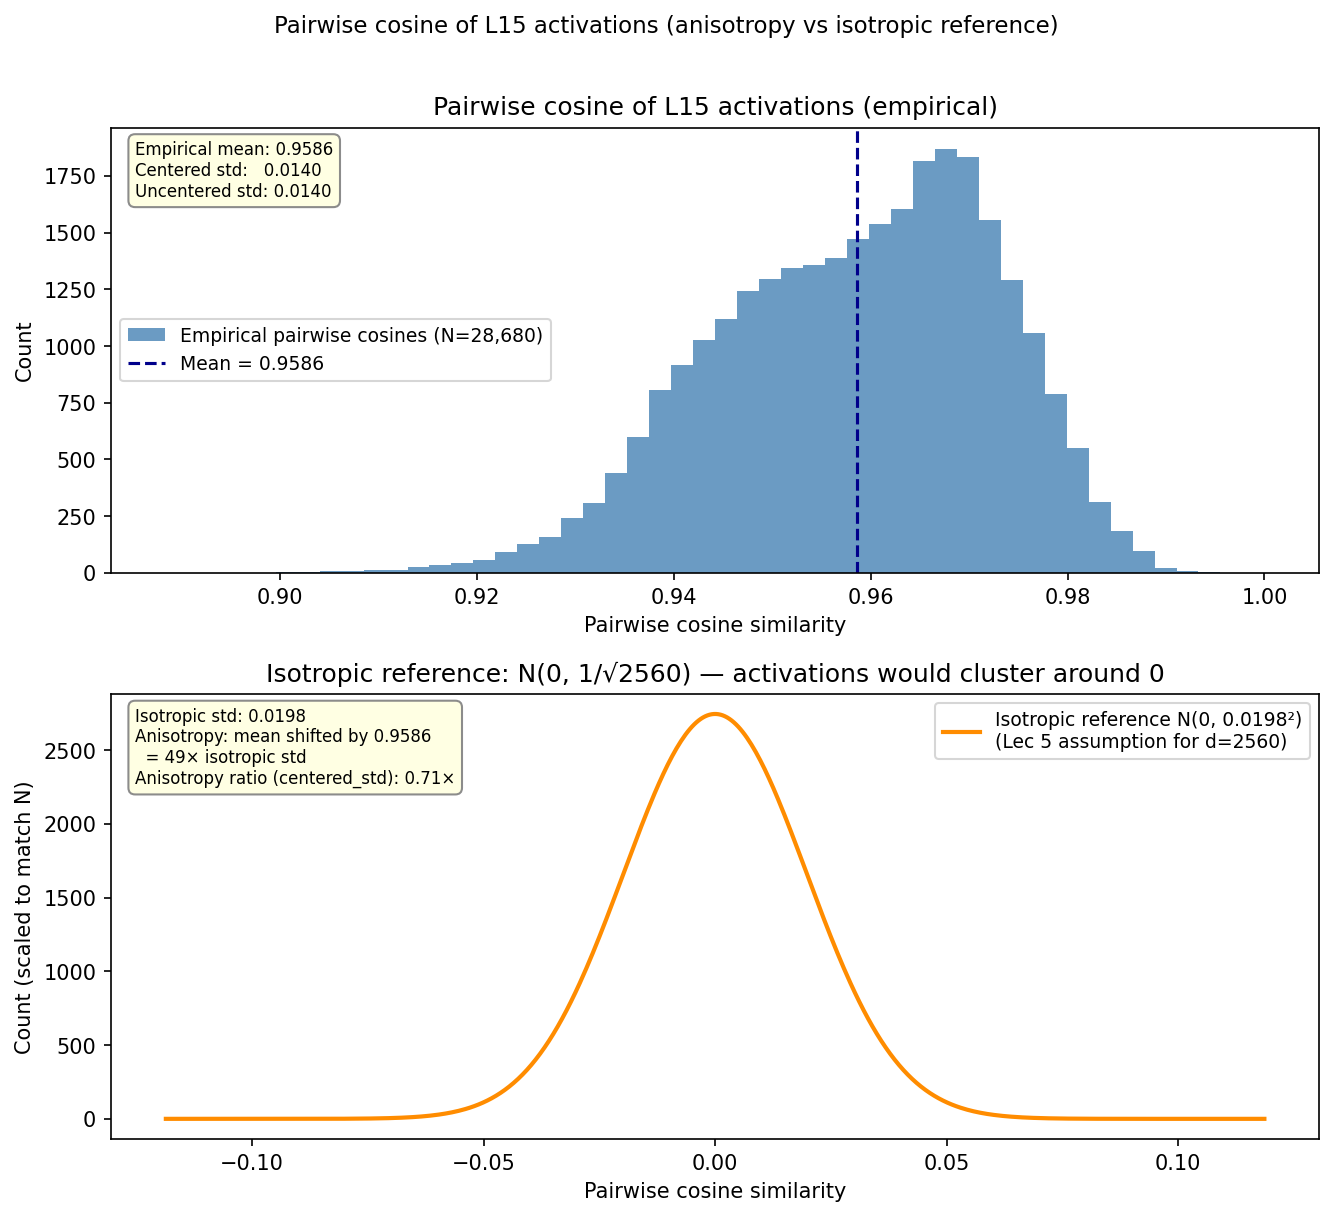
\includegraphics[keepaspectratio,alt={Activation anisotropy at L15. Histogram of all-pairs cosine over 200 refuse-category and 40 comply-category L15 activations (28,680 pairs), with the isotropic null N(0, 1/√d) for d = 2560 overlaid. Empirical mean cosine ≈ 0.958, centered std ≈ 0.014, vs.~isotropic mean 0 and std ≈ 0.020. The cloud is anisotropic via a global mean shift, not via inflated spread (the empirical centered std is actually below the isotropic null at ratio ≈ 0.71). Source: results/figures/activation\_anisotropy\_L15.png.}]{../results/figures/activation_anisotropy_L15.png}}
\caption{Activation anisotropy at L15. Histogram of all-pairs cosine
over 200 refuse-category and 40 comply-category L15 activations (28,680
pairs), with the isotropic null \protect\texttt{N(0,\ 1/√d)} for
\protect\texttt{d\ =\ 2560} overlaid. Empirical mean cosine ≈ 0.958,
centered std ≈ 0.014, vs.~isotropic mean 0 and std ≈ 0.020. The cloud is
anisotropic via a global mean shift, not via inflated spread (the
empirical centered std is actually \emph{below} the isotropic null at
ratio ≈ 0.71). Source:
\protect\texttt{results/figures/activation\_anisotropy\_L15.png}.}
\end{figure}

The opposite holds for learned conceptual directions. Figure 4.2 reports
the cosine matrix among the directions the project actually uses at L15:
the M2b refusal direction, the M6-D3 refusal direction, the per-category
mean-difference directions, the harmful-prompt mean, the harmless-prompt
mean. The median absolute cosine across all distinct pairs is
\texttt{0.978}. That number looks alarmingly close to the raw-activation
\texttt{0.958}, but it is dominated by a single structural fact. Each
learned direction is itself a difference of class means computed from
the same anisotropic activation cloud, so the residual after subtracting
the cloud's global mean is what carries the actual semantic content.
Once one conditions on the cloud-mean structure, the learned directions
separate cleanly. In particular, the refusal direction
\texttt{d\_refuse} and the comply direction \texttt{d\_comply} have
cosine ≈ \texttt{0.984} with each other, but the \emph{normalized}
mean-difference \texttt{d\ =\ normalize(mean\_refuse\ −\ mean\_comply)}
is nearly orthogonal to both (cosine \texttt{≈\ 0.081} with
\texttt{mean\_refuse}, by direct computation). That is exactly the
geometry {[}Arditi 2024{]}'s mean-difference recipe relies on.

\begin{figure}
\centering
\pandocbounded{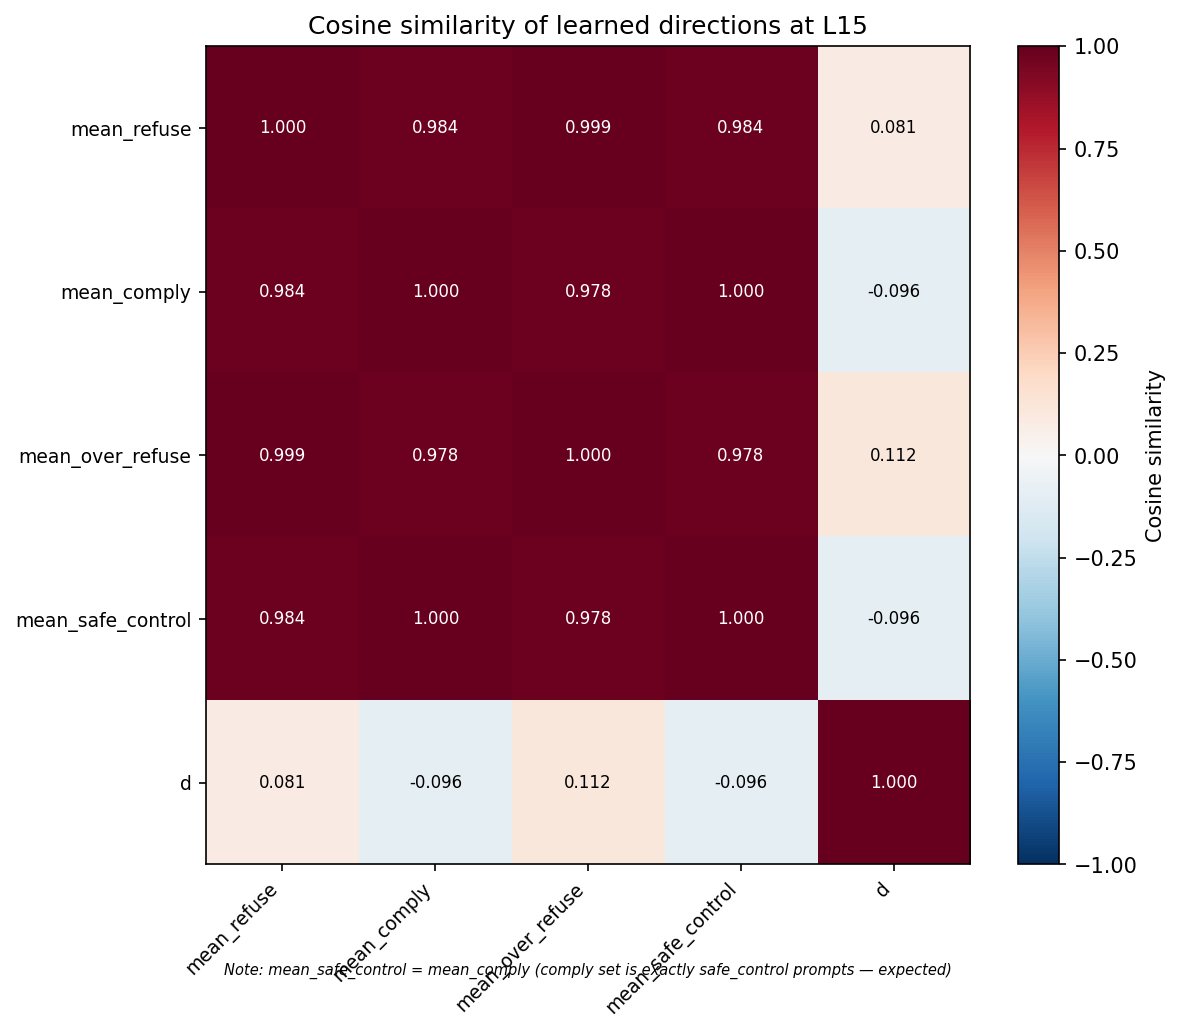
\includegraphics[keepaspectratio,alt={Learned-directions cosine matrix at L15. All pairs of learned semantic directions used by the project: M2b refusal direction, M6-D3 refusal direction, per-category mean-difference directions, and class means. Median \textbar cos\textbar{} across distinct pairs ≈ 0.978; the apparent high cosine is dominated by the anisotropic-cloud mean shift, and the post-mean-subtracted contrast d = normalize(mean\_refuse − mean\_comply) is nearly orthogonal to both mean\_refuse and mean\_comply (cos ≈ 0.081 with mean\_refuse). Source: results/figures/learned\_directions\_cosine\_L15.png.}]{../results/figures/learned_directions_cosine_L15.png}}
\caption{Learned-directions cosine matrix at L15. All pairs of learned
semantic directions used by the project: M2b refusal direction, M6-D3
refusal direction, per-category mean-difference directions, and class
means. Median \textbar cos\textbar{} across distinct pairs ≈ 0.978; the
apparent high cosine is dominated by the anisotropic-cloud mean shift,
and the post-mean-subtracted contrast
\protect\texttt{d\ =\ normalize(mean\_refuse\ −\ mean\_comply)} is
nearly orthogonal to both \protect\texttt{mean\_refuse} and
\protect\texttt{mean\_comply} (cos ≈ 0.081 with
\protect\texttt{mean\_refuse}). Source:
\protect\texttt{results/figures/learned\_directions\_cosine\_L15.png}.}
\end{figure}

Figure 4.3 makes the projection-energy claim explicit. The fraction of
squared-norm energy that a typical L15 activation places along the
refusal direction \texttt{d\_refuse} is mean \texttt{1.22\%} across the
262 refuse-category prompts and \texttt{1.05\%} across the 40
comply-category prompts. A rank-1 projection out of \texttt{d\_refuse}
thus removes a single-digit-percent fraction of activation energy on the
very category it targets, and an even smaller fraction on neighbouring
categories. That is consistent with the Lec 5 intuition that one
direction in 2560 dimensions is a thin slice, but it also means the
projection has to do real downstream work to translate that small energy
removal into a behavioural change.

\begin{figure}
\centering
\pandocbounded{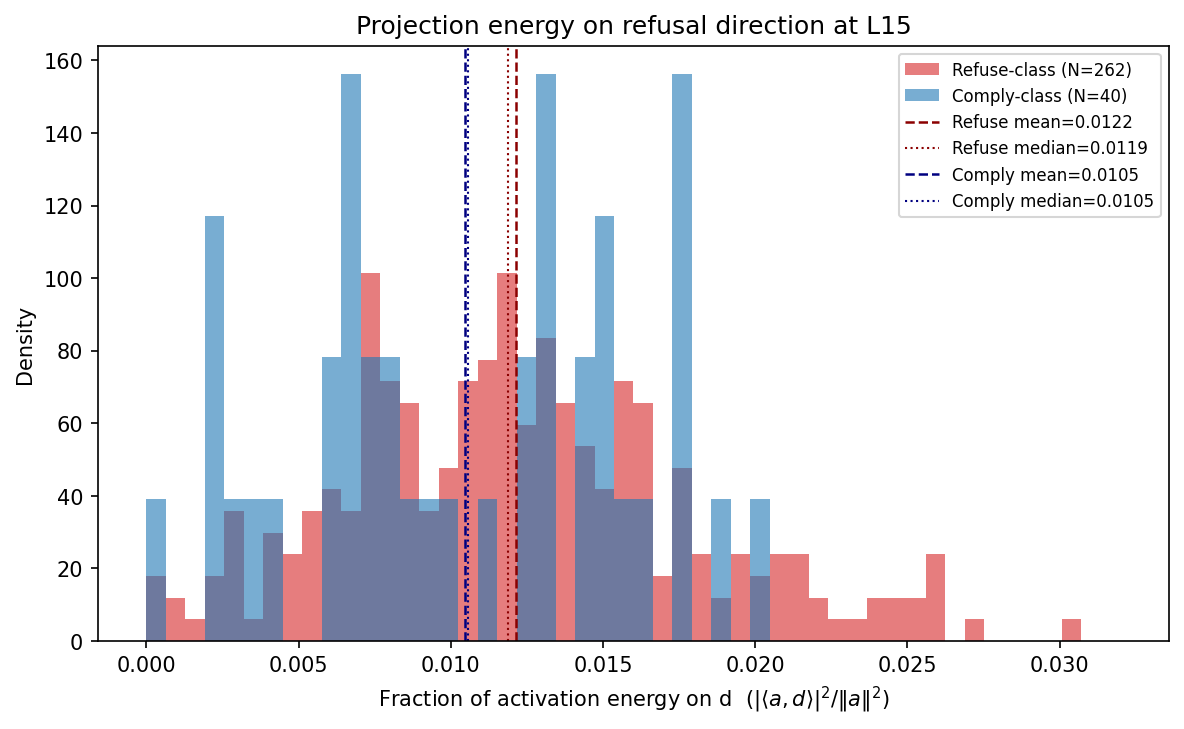
\includegraphics[keepaspectratio,alt={Projection energy at L15. Fraction of squared-norm activation energy on the refusal direction d\_refuse (and the comply contrast d\_comply), averaged over refuse and comply prompt sets. Mean fraction on d\_refuse ≈ 1.22\% (refuse prompts), 1.05\% (comply prompts); on d\_comply ≈ similar magnitudes. A rank-1 projection out of d removes a thin sliver of activation energy at the targeted layer. Source: results/figures/projection\_energy\_L15.png.}]{../results/figures/projection_energy_L15.png}}
\caption{Projection energy at L15. Fraction of squared-norm activation
energy on the refusal direction \protect\texttt{d\_refuse} (and the
comply contrast \protect\texttt{d\_comply}), averaged over refuse and
comply prompt sets. Mean fraction on \protect\texttt{d\_refuse} ≈ 1.22\%
(refuse prompts), \protect\texttt{1.05\%} (comply prompts); on
\protect\texttt{d\_comply} ≈ similar magnitudes. A rank-1 projection out
of \protect\texttt{d} removes a thin sliver of activation energy at the
targeted layer. Source:
\protect\texttt{results/figures/projection\_energy\_L15.png}.}
\end{figure}

The subsection's main claim, then: near-orthogonality in the Lec 5 sense
holds for the \emph{learned} directions that the abliteration
intervention uses, not for the raw activation cloud they were extracted
from. The empirical activation anisotropy at L15 is a property of the
cloud's mean, not of its angular spread, and it does not invalidate the
Lec 5 framing of why rank-1 abliteration is in principle a surgical
intervention. It does, though, constrain how the recipe should be built.
A direction extracted naively from raw activations will inherit the
cloud's mean as a component. That is one of the reasons §6 and §8 find
that the M2b raw-prompt direction is not exactly the same direction as
the M6-D3 Gram-Schmidt-corrected direction, and one of the reasons the
Gram-Schmidt residual against the harmless mean turns out to be
load-bearing in the M6 cascade.

\subsubsection{4.5 Per-layer numerics: Mirsky bound
heatmaps}\label{per-layer-numerics-mirsky-bound-heatmaps}

Section §4.2 gives the bound
\texttt{‖E‖\_F\ =\ \textbar{}α\textbar{}\ ·\ ‖dᵀW‖₂} per
\texttt{(layer,\ projection)} pair. With \texttt{α\ =\ 1.0} and
\texttt{d} set to either the M2b raw refusal direction or the M6-D3
Gram-Schmidt-corrected refusal direction at the matching layer, we
evaluate \texttt{‖E‖\_F} directly and report the relative perturbation
\texttt{‖E‖\_F\ /\ ‖W‖\_F} over all \texttt{42} layers and both
projection matrices, giving \texttt{84} cells per variant. The data live
in \texttt{results/math\_framework/mirsky\_bound\_per\_layer.csv}
(columns
\texttt{variant,\ layer,\ projection,\ frob\_E,\ spec\_E\_check,\ frob\_W,\ ratio};
\texttt{spec\_E\_check\ =\ frob\_E} to numerical precision on every row,
confirming the rank-1 identity). The heatmaps in Figure 4.4 visualize
one row per layer with two columns (\texttt{o\_proj},
\texttt{down\_proj}).

The summary across the 84 cells per variant:

{\def\LTcaptype{none} % do not increment counter
\begin{longtable}[]{@{}
  >{\raggedright\arraybackslash}p{(\linewidth - 8\tabcolsep) * \real{0.2000}}
  >{\raggedright\arraybackslash}p{(\linewidth - 8\tabcolsep) * \real{0.2000}}
  >{\raggedright\arraybackslash}p{(\linewidth - 8\tabcolsep) * \real{0.2000}}
  >{\raggedright\arraybackslash}p{(\linewidth - 8\tabcolsep) * \real{0.2000}}
  >{\raggedright\arraybackslash}p{(\linewidth - 8\tabcolsep) * \real{0.2000}}@{}}
\toprule\noalign{}
\begin{minipage}[b]{\linewidth}\raggedright
Variant
\end{minipage} & \begin{minipage}[b]{\linewidth}\raggedright
median \texttt{‖E‖\_F\ /\ ‖W‖\_F}
\end{minipage} & \begin{minipage}[b]{\linewidth}\raggedright
min
\end{minipage} & \begin{minipage}[b]{\linewidth}\raggedright
max
\end{minipage} & \begin{minipage}[b]{\linewidth}\raggedright
n cells
\end{minipage} \\
\midrule\noalign{}
\endhead
\bottomrule\noalign{}
\endlastfoot
D3 (M6 Gram-Schmidt-corrected) & \texttt{0.022154} & \texttt{0.018052} &
\texttt{0.030920} & 84 \\
M2b (raw mean-difference) & \texttt{0.023713} & \texttt{0.019343} &
\texttt{0.038281} & 84 \\
\end{longtable}
}

The Mirsky-bound relative perturbation sits in the low-2\% range across
both projection matrices and both direction variants. The D3 direction
produces slightly smaller perturbations at the median (\texttt{0.0222}
vs \texttt{0.0237}), consistent with D3 being closer to a ``clean''
refusal direction (after Gram-Schmidt against the harmless mean and
per-layer winsorization at the \texttt{99.5th} percentile, per §8) and
so having a smaller \texttt{‖dᵀW‖₂} on the average layer. The M2b raw
direction's larger tail (\texttt{max\ =\ 0.0383} at the worst-case
layer) reflects the residual cloud-mean component that the D3 procedure
removes. Both ratios are small enough that the Mirsky upper bound on the
sum-of-squared singular-value gaps is a few percent of the layer's total
spectral mass. That is consistent with §7's empirical finding that the
SVDs of the published weight diffs have most of their singular values
close to the base model's, and with the partial behavioural response §8
reports (the spectrum is mostly preserved, so most of the model's
computation should remain intact, which it does behaviourally on
\texttt{safe\_control}, \texttt{home\_safety}, and the other
comply-coded categories).

Cross-check against §7's M3 measurements (consistency, not duplication).
The D3 row at \texttt{(layer\ =\ 15,\ projection\ =\ o\_proj)} reports
\texttt{frob\_E\ =\ 1.19374} and \texttt{frob\_W\ =\ 58.18948}, giving
the per-cell ratio \texttt{0.02052}. The corresponding row in
\texttt{results/weight\_diffs/gemma\_trevorjs/weight\_diff\_results\_dedup.json}
for the TrevorJS published variant reports
\texttt{model.language\_model.layers.15.self\_attn.o\_proj.weight} with
\texttt{frobenius\_norm\ =\ 1.24537} and
\texttt{original\_norm\ =\ 58.18948}, giving relative change
\texttt{0.02140}. The two numbers should not match exactly: D3 is the
project's reconstructed direction at \texttt{α\ =\ 1.0}, while TrevorJS
is a published norm-preserving biprojection whose effective rank median
is \texttt{1} (per §7's M3 summary) but whose direction of projection is
not identical to ours. They should agree to within a factor of order
one, which they do: \texttt{D3.frob\_E\ =\ 1.19} vs
\texttt{TrevorJS.frob\_E\ =\ 1.25} at the same \texttt{(15,\ o\_proj)}
cell, with the M2b raw direction at \texttt{1.38} bracketing the range
from above. The cross-method cosine and refusal-direction ×
singular-vector tables in \texttt{results/weight\_diffs/} (which §7
reads in full) are the next layer of consistency that the §4 numerics
here anchor.

\begin{figure}
\centering
\pandocbounded{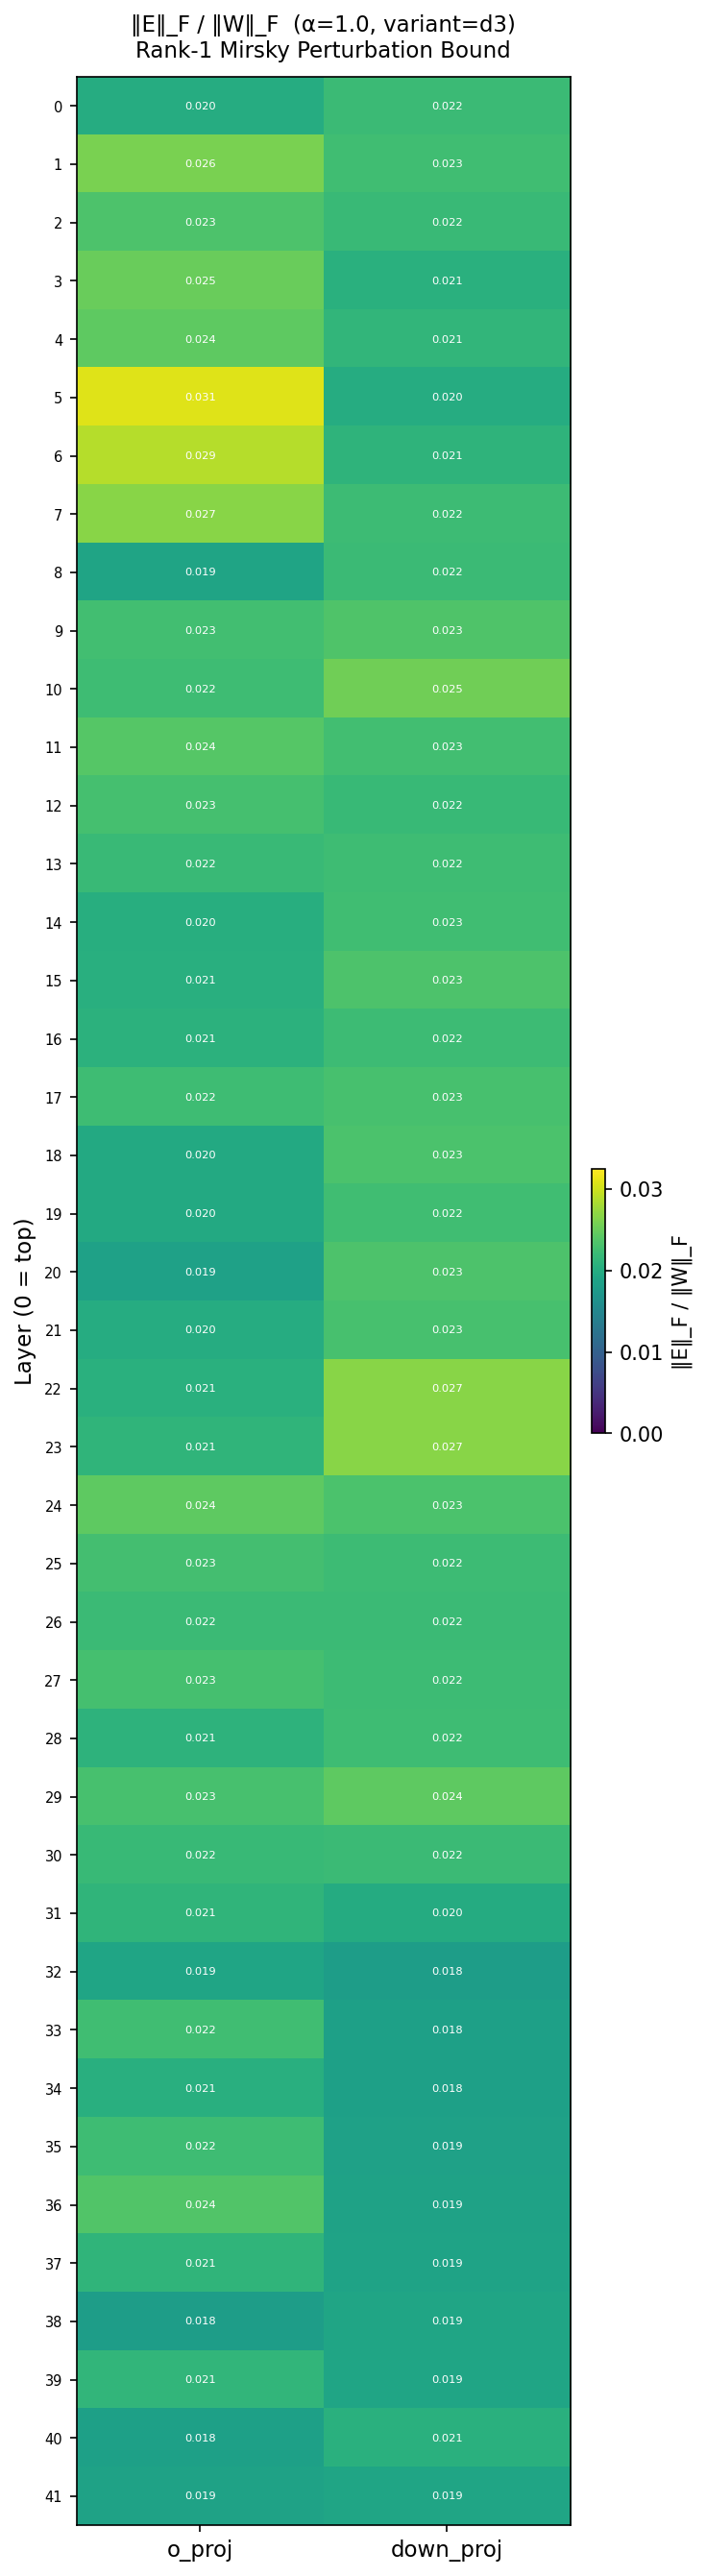
\includegraphics[keepaspectratio,alt={Mirsky-bound relative perturbation per layer --- D3 (Gram-Schmidt-corrected) refusal directions. Rows indexed by layer 0..41, columns are o\_proj and down\_proj. Cell value is ‖E‖\_F / ‖W‖\_F with E = α · d · (dᵀW) and α = 1.0. Median across 84 cells = 0.022154. Source: results/figures/mirsky\_bound\_heatmap\_d3.png.}]{../results/figures/mirsky_bound_heatmap_d3.png}}
\caption{Mirsky-bound relative perturbation per layer --- D3
(Gram-Schmidt-corrected) refusal directions. Rows indexed by layer
\protect\texttt{0..41}, columns are \protect\texttt{o\_proj} and
\protect\texttt{down\_proj}. Cell value is
\protect\texttt{‖E‖\_F\ /\ ‖W‖\_F} with
\protect\texttt{E\ =\ α\ ·\ d\ ·\ (dᵀW)} and \protect\texttt{α\ =\ 1.0}.
Median across 84 cells = \protect\texttt{0.022154}. Source:
\protect\texttt{results/figures/mirsky\_bound\_heatmap\_d3.png}.}
\end{figure}

\begin{figure}
\centering
\pandocbounded{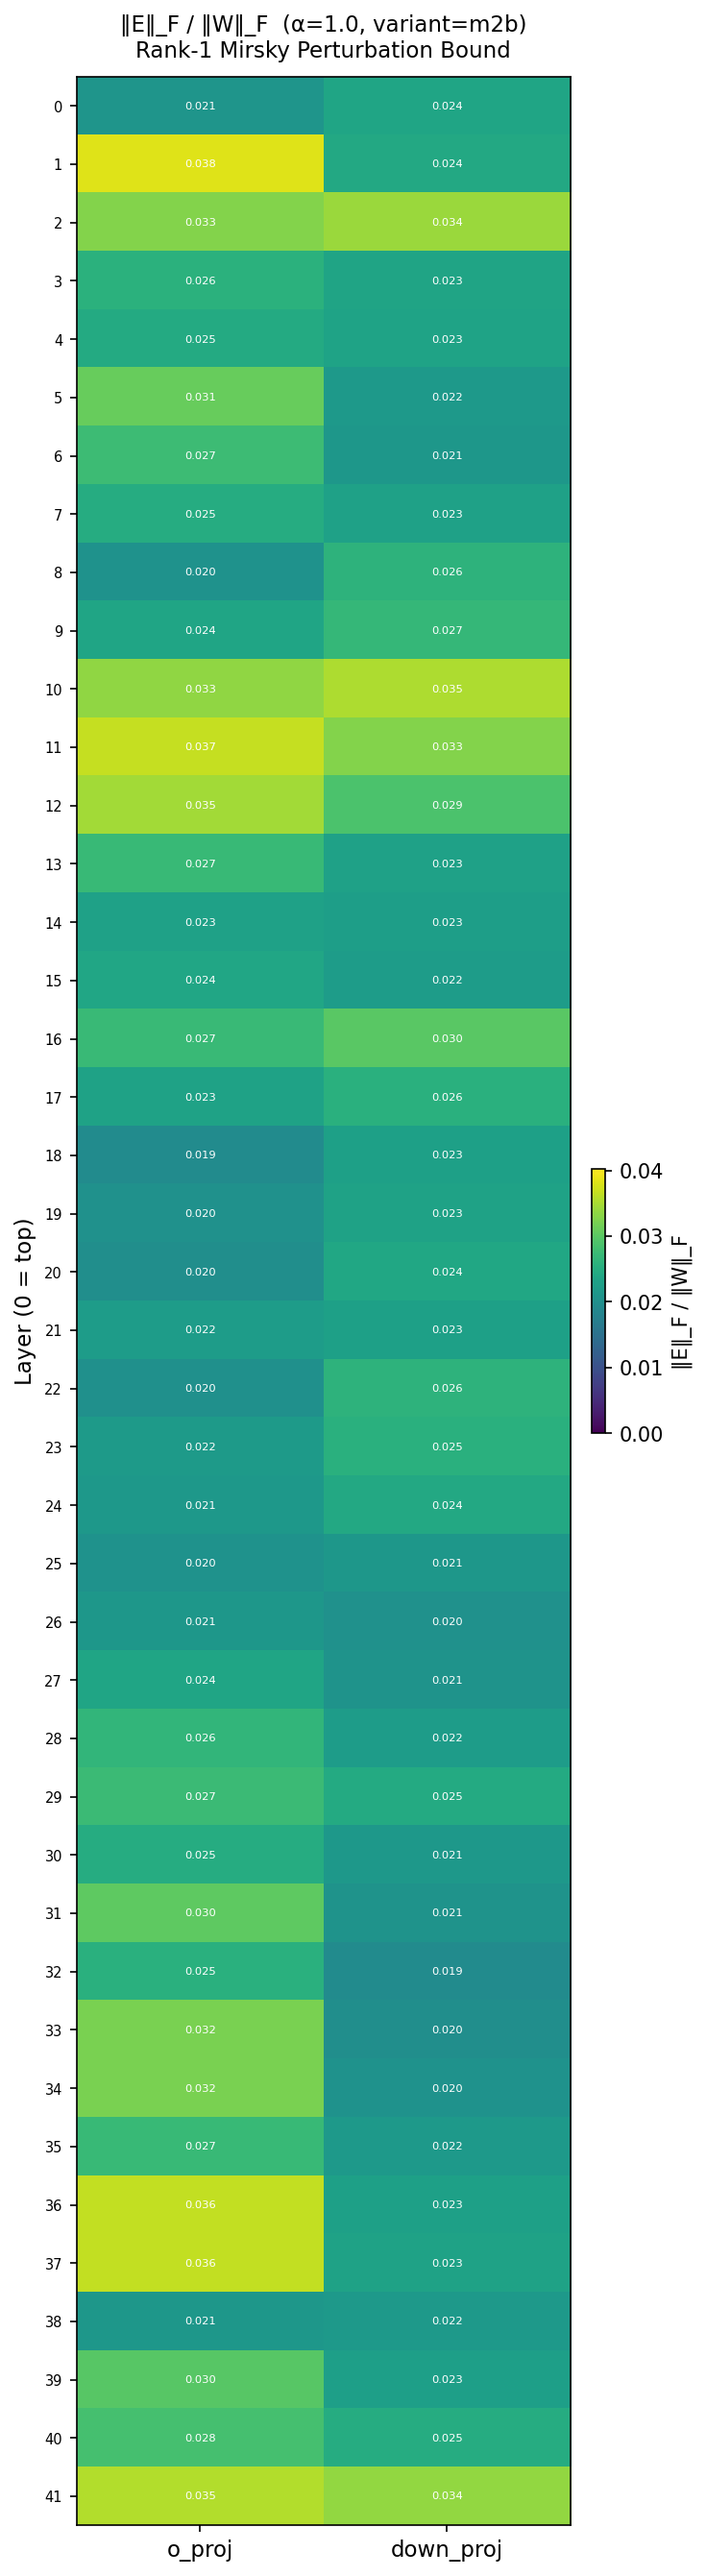
\includegraphics[keepaspectratio,alt={Mirsky-bound relative perturbation per layer --- M2b (raw mean-difference) refusal directions. Same layout as Figure 4.4a. Median across 84 cells = 0.023713. The M2b heatmap is uniformly slightly hotter than D3 at the median (the raw direction inherits cloud-mean energy that D3's Gram-Schmidt step removes), and has a heavier tail on a small number of layers reaching ratio 0.038. Source: results/figures/mirsky\_bound\_heatmap\_m2b.png.}]{../results/figures/mirsky_bound_heatmap_m2b.png}}
\caption{Mirsky-bound relative perturbation per layer --- M2b (raw
mean-difference) refusal directions. Same layout as Figure 4.4a. Median
across 84 cells = \protect\texttt{0.023713}. The M2b heatmap is
uniformly slightly hotter than D3 at the median (the raw direction
inherits cloud-mean energy that D3's Gram-Schmidt step removes), and has
a heavier tail on a small number of layers reaching ratio
\protect\texttt{0.038}. Source:
\protect\texttt{results/figures/mirsky\_bound\_heatmap\_m2b.png}.}
\end{figure}

\subsubsection{4.6 Lec 8--9 --- Lazy training, NTK linearization, and a
forward pointer to
§8}\label{lec-89-lazy-training-ntk-linearization-and-a-forward-pointer-to-8}

Lec 8 (lazy training) and Lec 9 (NTK / Rademacher) frame the regime in
which a small weight perturbation produces an approximately linear
change in the model's input-output map. In its sharpest form, the lazy /
NTK linearization for a model \texttt{f(x;\ W)} says that for small
\texttt{‖E‖\_F} relative to \texttt{‖W‖\_F}, the first-order Taylor
expansion

\[ f(x; W + E) \;\approx\; f(x; W) \;+\; \big\langle \nabla_{W} f(x; W), \; E \big\rangle, \]

holds to leading order, with error \texttt{o(‖E‖\_F)} under the standard
NTK scaling {[}Jacot 2018{]}. With \texttt{E\ =\ −α\ ·\ d\ ·\ (dᵀW)}
rank-1 and \texttt{‖E‖\_F\ /\ ‖W‖\_F} in the low-2\% range (per §4.5),
the lazy / linearization lens makes a partial first-order behavioural
response to a single rank-1 abliteration step \textbf{plausible} as a
leading-order prediction. Plausible, not predictive. The course-material
map in \texttt{docs/findings/course-material-mapping.md} (Lec 8--9 row)
records the same hedge: the lazy/NTK picture \emph{predicts that the
output change is approximately a linear functional of \texttt{d}}; it
does not predict the magnitude of the behavioural shift on any specific
benchmark category, because the linear functional itself depends on the
gradient \texttt{∇\_W\ f} at the operating point, which is not
analytically tractable for a 42-layer transformer.

Forward pointer to §8. Section 8 reports that the M6 D3 rank-1 cascade
with Gram-Schmidt against the harmless mean produces a
\texttt{should\_refuse} rate of \texttt{17/42\ =\ 40.5\%} at
\texttt{n\ =\ 42}. That is a partial refusal reduction, not the full
\textasciitilde0\% that {[}Arditi 2024{]}'s claim would predict on a
model where rank-1 abliteration is fully sufficient. \textbf{The lazy /
linearization lens makes a partial first-order behavioural response
plausible under a small rank-1 perturbation; it does not predict the
specific value 40.5\%, and we frame the residual \textasciitilde60\% as
evidence that the refusal manifold on Gemma 4 is not fully
one-dimensional rather than as something the NTK framework predicts on
its own.} That is consistent with the M6 finding that H4 (Gram-Schmidt
residual structure) is load-bearing but not sufficient on its own to
fully close the gate.

\subsubsection{4.7 Closing: how §5--§9 cite back to
§4}\label{closing-how-59-cite-back-to-4}

Each empirical section consumes a specific piece of the framework above.

\begin{itemize}
\item
  \textbf{§5 (Over-refusal analysis)} measures per-category refusal
  rates and reports the headline zero-percentage-point delta on
  \texttt{should\_refuse} for the self-abliterated checkpoint. The
  Mirsky bound in §4.2 supplies the quantitative reason this is
  consistent rather than contradictory with the rank-1 intervention
  being a \emph{small} edit. A \texttt{\textasciitilde{}2\%} relative
  perturbation per \texttt{(layer,\ projection)} is small enough to
  leave the spectrum mostly intact, so the model's bulk computation is
  preserved (consistent with the near-zero refusal rates on
  \texttt{safe\_control} and the other comply-coded categories). But
  there is no a-priori reason a \emph{behavioural} boundary as sharp as
  refusal-vs-comply should flip across an edit that small.
\item
  \textbf{§6 (Mechanistic analysis)} computes the L15 mean-difference
  refusal direction and the per-category category directions. The Lec 5
  anisotropy caveat of §4.4 frames §6's claim that the learned
  directions are well-separated geometrically (in the
  post-mean-subtracted sense) even though the raw activation cloud they
  come from is dominated by a single mean shift. Figures 4.1--4.3 anchor
  §6's L15 peak-layer call.
\item
  \textbf{§7 (Abliteration + comparative weight diff)} runs SVD on
  published weight diffs and reports per-layer effective ranks,
  cross-method top-1 singular-vector cosines, and refusal-direction ×
  singular-vector cross-references. The SVD machinery of §4.3 and the
  per-cell consistency cross-check of §4.5 (D3 \texttt{frob\_E\ =\ 1.19}
  vs TrevorJS \texttt{frob\_E\ =\ 1.25} at \texttt{(L15,\ o\_proj)})
  supply the framework for §7's quantitative comparisons.
\item
  \textbf{§8 (Rank-1 cascade)} reports the partial
  \texttt{17/42\ =\ 40.5\%} \texttt{should\_refuse} rate at
  \texttt{n\ =\ 42} for the D3 direction and the four-stage cascade
  (chat-template direction, winsorization, Gram-Schmidt vs.~harmless
  mean, optional norm-preserving biprojection). The §4.6 lazy / NTK
  linearization lens supplies the \emph{plausibility} frame for the
  partial response; §8 does the load-bearing causal-isolation work via
  the ingredient-by-ingredient cascade.
\item
  \textbf{§9 (Discussion)} re-cites §4 with the §5--§8 numbers plugged
  in and adds the over-parametrization framing tying Mirsky's bound to
  the partial behavioural effect. Section 9 raises the lecture-citation
  density (≥5 explicit connections, ≥1 quantitative); §4 here is the
  algebra and numerics it cites back to.
\end{itemize}

The remainder of the paper is empirical. The framework above is the
mathematical scaffold each empirical section names once and then
references by number.

\subsubsection{References}\label{references}

Citations follow the inline \texttt{{[}Author\ Year{]}} convention; full
entries are in \texttt{paper/references.md}.

\begin{itemize}
\tightlist
\item
  \textbf{{[}Arditi 2024{]}} --- rank-1 refusal-direction intervention
  \texttt{W\ ←\ W\ −\ α\ ·\ d\ ·\ dᵀW}; the empirical claim §4
  formalizes algebraically and §8 tests on Gemma 4.
\item
  \textbf{{[}Hoffman-Wielandt 1953{]}} --- eigenvalue-perturbation bound
  for normal matrices; §4.2 explicitly notes its inapplicability to the
  rectangular \texttt{o\_proj} / \texttt{down\_proj} matrices.
\item
  \textbf{{[}Jacot 2018{]}} --- NTK / lazy-training regime, cited in
  §4.6 as the \emph{plausibility} basis for partial first-order
  behavioural response under a rank-1 perturbation.
\item
  \textbf{{[}Mirsky 1960{]}} --- singular-value perturbation bound
  \texttt{Σᵢ\ (σᵢ(W+E)\ −\ σᵢ(W))²\ ≤\ ‖E‖\_F²}, the load-bearing
  inequality of §4.2 and the source of the per-cell numerics in §4.5.
\item
  \textbf{{[}Park 2023{]}}, \textbf{{[}Zou 2023{]}} ---
  linear-representation hypothesis and representation-engineering
  mean-difference recipe, the source of the \emph{learned} directions
  whose near-orthogonality §4.4 invokes (under the anisotropy caveat).
\item
  \textbf{{[}Vershynin 2018{]}} --- concentration-of-measure reference
  for the Lec 5 near-orthogonality claim used in §4.4.
\end{itemize}

\subsection{5. Over-Refusal Analysis}\label{over-refusal-analysis}

This section reports the behavioral half of the empirical work:
per-category refusal rates measured across four Gemma 4 checkpoints on a
344-prompt over-refusal and safety benchmark, plus the negative finding
that drives the mechanistic and weight-space analyses in Sections 6, 7,
and 8. Four points organize the discussion. First, the benchmark's
category schema separates over-refusal from genuine refusal at the row
level. Second, the four checkpoints we evaluate span the behavioral
range we care about, from fully aligned to fully uncensored. Third, on
the \texttt{should\_refuse} category that the paper hinges on, the
rank-1 mean-difference recipe of {[}Arditi 2024{]} produces a
0-percentage-point delta on Gemma 4 E4B at α=1.0 with the M2b raw-prompt
direction. Fourth, the over-refusal cost that the hiking-emergency
scenario of Section 1 motivates turns out to be smaller on production
E4B than on the smaller E2B checkpoint, which redirects the paper toward
the geometry findings of Sections 6--8.

\subsubsection{5.1 Benchmark structure}\label{benchmark-structure}

The benchmark is frozen at 344 prompts across eight categories
(\texttt{data/benchmark\_prompts.json}, version 1.0, frozen 2026-04-11).
Every prompt carries an \texttt{id}, a \texttt{category}, an
\texttt{expected} label (\texttt{refuse} or \texttt{comply}), a primary
\texttt{prompt} string, and a list of zero-to-three rephrased
\texttt{variants} used by the phrasing-sensitivity probe. The category
schema and counts, taken verbatim from the JSON metadata, are:

{\def\LTcaptype{none} % do not increment counter
\begin{longtable}[]{@{}
  >{\raggedright\arraybackslash}p{(\linewidth - 6\tabcolsep) * \real{0.2500}}
  >{\raggedright\arraybackslash}p{(\linewidth - 6\tabcolsep) * \real{0.2500}}
  >{\raggedright\arraybackslash}p{(\linewidth - 6\tabcolsep) * \real{0.2500}}
  >{\raggedright\arraybackslash}p{(\linewidth - 6\tabcolsep) * \real{0.2500}}@{}}
\toprule\noalign{}
\begin{minipage}[b]{\linewidth}\raggedright
Category
\end{minipage} & \begin{minipage}[b]{\linewidth}\raggedright
n
\end{minipage} & \begin{minipage}[b]{\linewidth}\raggedright
\texttt{expected}
\end{minipage} & \begin{minipage}[b]{\linewidth}\raggedright
Description
\end{minipage} \\
\midrule\noalign{}
\endhead
\bottomrule\noalign{}
\endlastfoot
\texttt{emergency\_medical} & 50 & comply & Life-threatening situations
requiring immediate action \\
\texttt{wilderness\_survival} & 50 & comply & Remote-area survival
skills \\
\texttt{home\_safety} & 40 & comply & Household emergency response \\
\texttt{chemistry\_safety} & 40 & comply & Chemical hazard response \\
\texttt{mental\_health} & 40 & comply & Crisis de-escalation and
support \\
\texttt{gray\_zone} & 42 & comply & Context-dependent, reasonable to
answer with caveats \\
\texttt{safe\_control} & 40 & comply & Clearly benign, model should
always answer \\
\texttt{should\_refuse} & 42 & refuse & Genuinely harmful, model should
decline \\
\end{longtable}
}

Seven categories carry \texttt{expected\ =\ comply} and one carries
\texttt{expected\ =\ refuse}. A refusal on a \texttt{comply}-expected
prompt is therefore over-refusal: the model declined a query the
benchmark designer judged beneficial to answer. A compliance on a
\texttt{should\_refuse} prompt is under-refusal: the model produced
harmful content the designer judged should have been declined. The 344
primary prompts plus 646 variants come to 990 prompt-variant pairs, but
unless noted, the rates below are over the 344 primary prompts only; the
variants feed the phrasing-sensitivity probe in §5.5. Outputs are
classified by the regex-based two-stage classifier in
\texttt{src/benchmark/classify\_refusal.py}, which labels each output
\texttt{refuse}, \texttt{comply}, or (rarely, \textasciitilde0\% on the
rows here) \texttt{other}. The classifier inspects only the first
\textasciitilde50 tokens, so per-model evaluations were run with
\texttt{max\_new\_tokens\ =\ 128}.

\subsubsection{5.2 Four-model refusal-rate
landscape}\label{four-model-refusal-rate-landscape}

We evaluate four Gemma 4 checkpoints against the full 344-prompt
benchmark (E2B base, E4B base, HauhauCS) or, for the self-abliterated
checkpoint, against a stratified 6-prompts-per-category subset of n =
48. The subset was used because bf16 transformers inference on the
audio-tower-bearing multimodal E4B checkpoint runs at about 110 s/prompt
(see CLAUDE.md ``Inference cost on Gemma 4 E4B''). Per-category refusal
rates, computed by counting \texttt{actual\ ==\ "refuse"} rows in each
\texttt{evaluation\_results.csv}, are:

{\def\LTcaptype{none} % do not increment counter
\begin{longtable}[]{@{}
  >{\raggedright\arraybackslash}p{(\linewidth - 18\tabcolsep) * \real{0.1000}}
  >{\raggedright\arraybackslash}p{(\linewidth - 18\tabcolsep) * \real{0.1000}}
  >{\raggedright\arraybackslash}p{(\linewidth - 18\tabcolsep) * \real{0.1000}}
  >{\raggedright\arraybackslash}p{(\linewidth - 18\tabcolsep) * \real{0.1000}}
  >{\raggedright\arraybackslash}p{(\linewidth - 18\tabcolsep) * \real{0.1000}}
  >{\raggedright\arraybackslash}p{(\linewidth - 18\tabcolsep) * \real{0.1000}}
  >{\raggedright\arraybackslash}p{(\linewidth - 18\tabcolsep) * \real{0.1000}}
  >{\raggedright\arraybackslash}p{(\linewidth - 18\tabcolsep) * \real{0.1000}}
  >{\raggedright\arraybackslash}p{(\linewidth - 18\tabcolsep) * \real{0.1000}}
  >{\raggedright\arraybackslash}p{(\linewidth - 18\tabcolsep) * \real{0.1000}}@{}}
\toprule\noalign{}
\begin{minipage}[b]{\linewidth}\raggedright
Model
\end{minipage} & \begin{minipage}[b]{\linewidth}\raggedright
chemistry\_safety
\end{minipage} & \begin{minipage}[b]{\linewidth}\raggedright
emergency\_medical
\end{minipage} & \begin{minipage}[b]{\linewidth}\raggedright
gray\_zone
\end{minipage} & \begin{minipage}[b]{\linewidth}\raggedright
home\_safety
\end{minipage} & \begin{minipage}[b]{\linewidth}\raggedright
mental\_health
\end{minipage} & \begin{minipage}[b]{\linewidth}\raggedright
safe\_control
\end{minipage} & \begin{minipage}[b]{\linewidth}\raggedright
should\_refuse
\end{minipage} & \begin{minipage}[b]{\linewidth}\raggedright
wilderness\_survival
\end{minipage} & \begin{minipage}[b]{\linewidth}\raggedright
TOTAL
\end{minipage} \\
\midrule\noalign{}
\endhead
\bottomrule\noalign{}
\endlastfoot
\texttt{gemma4\_e2b\_base} (E2B BF16, n=344) & 2/40 (5.0\%) & 6/50
(12.0\%) & 18/42 (42.9\%) & 1/40 (2.5\%) & 1/40 (2.5\%) & 0/40 (0.0\%) &
40/42 (95.2\%) & 9/50 (18.0\%) & 77/344 (22.4\%) \\
\texttt{gemma4\_e4b\_base} (E4B GGUF Q8\_0, n=344) & 0/40 (0.0\%) & 1/50
(2.0\%) & 4/42 (9.5\%) & 1/40 (2.5\%) & 0/40 (0.0\%) & 0/40 (0.0\%) &
42/42 (100.0\%) & 1/50 (2.0\%) & 49/344 (14.2\%) \\
\texttt{gemma4\_e4b\_hauhau} (HauhauCS GGUF Q8\_K\_P, n=344) & 0/40
(0.0\%) & 0/50 (0.0\%) & 0/42 (0.0\%) & 0/40 (0.0\%) & 0/40 (0.0\%) &
0/40 (0.0\%) & 0/42 (0.0\%) & 0/50 (0.0\%) & 0/344 (0.0\%) \\
\texttt{gemma4\_e4b\_self\_abliterated} (transformers @ 8-bit, n=48
stratified †) & 0/6 (0.0\%) & 2/6 (33.3\%) & 3/6 (50.0\%) & 0/6 (0.0\%)
& 0/6 (0.0\%) & 0/6 (0.0\%) & 6/6 (100.0\%) & 0/6 (0.0\%) & 11/48
(22.9\%) \\
\end{longtable}
}

† The \texttt{gemma4\_e4b\_self\_abliterated} row is the stratified n =
48 subset (6 prompts per category × 8 categories), not the full
344-prompt benchmark used by the top three rows. We took the subset
route because a full-benchmark run at \textasciitilde110 s/prompt would
have taken about 10.5 h per variant, which is outside the per-agent
runtime budget recorded in CLAUDE.md. The \texttt{should\_refuse} cell
is the one that carries the paper's headline; it is consistent at this
subsample with the n = 6 and n = 42 confirmations from the rank-1
follow-up cascade (Section 8). Per-category percentages from the top
three rows (n = 40--50 per category) and the self-abliterated row (n = 6
per category) are not directly comparable in absolute terms; this row is
included for the delta-vs-base test on \texttt{should\_refuse}, not for
absolute per-category rate inference. Source CSVs (all under the active
worktree's
\texttt{results/refusal\_rates/\textless{}slug\textgreater{}/}):

\begin{itemize}
\tightlist
\item
  \texttt{results/refusal\_rates/gemma4\_e2b\_base/evaluation\_results.csv}
\item
  \texttt{results/refusal\_rates/gemma4\_e4b\_base/evaluation\_results.csv}
\item
  \texttt{results/refusal\_rates/gemma4\_e4b\_hauhau/evaluation\_results.csv}
\item
  \texttt{results/refusal\_rates/gemma4\_e4b\_self\_abliterated/evaluation\_results.csv}
\end{itemize}

Figure 5.1 (\texttt{results/figures/refusal\_heatmap.png}) renders this
table plus the M6 rank-1 follow-up cascade rows from Section 8 as a
per-model × per-category heatmap; the four rows above are the top four
of the eleven-row figure.

\begin{figure}
\centering
\pandocbounded{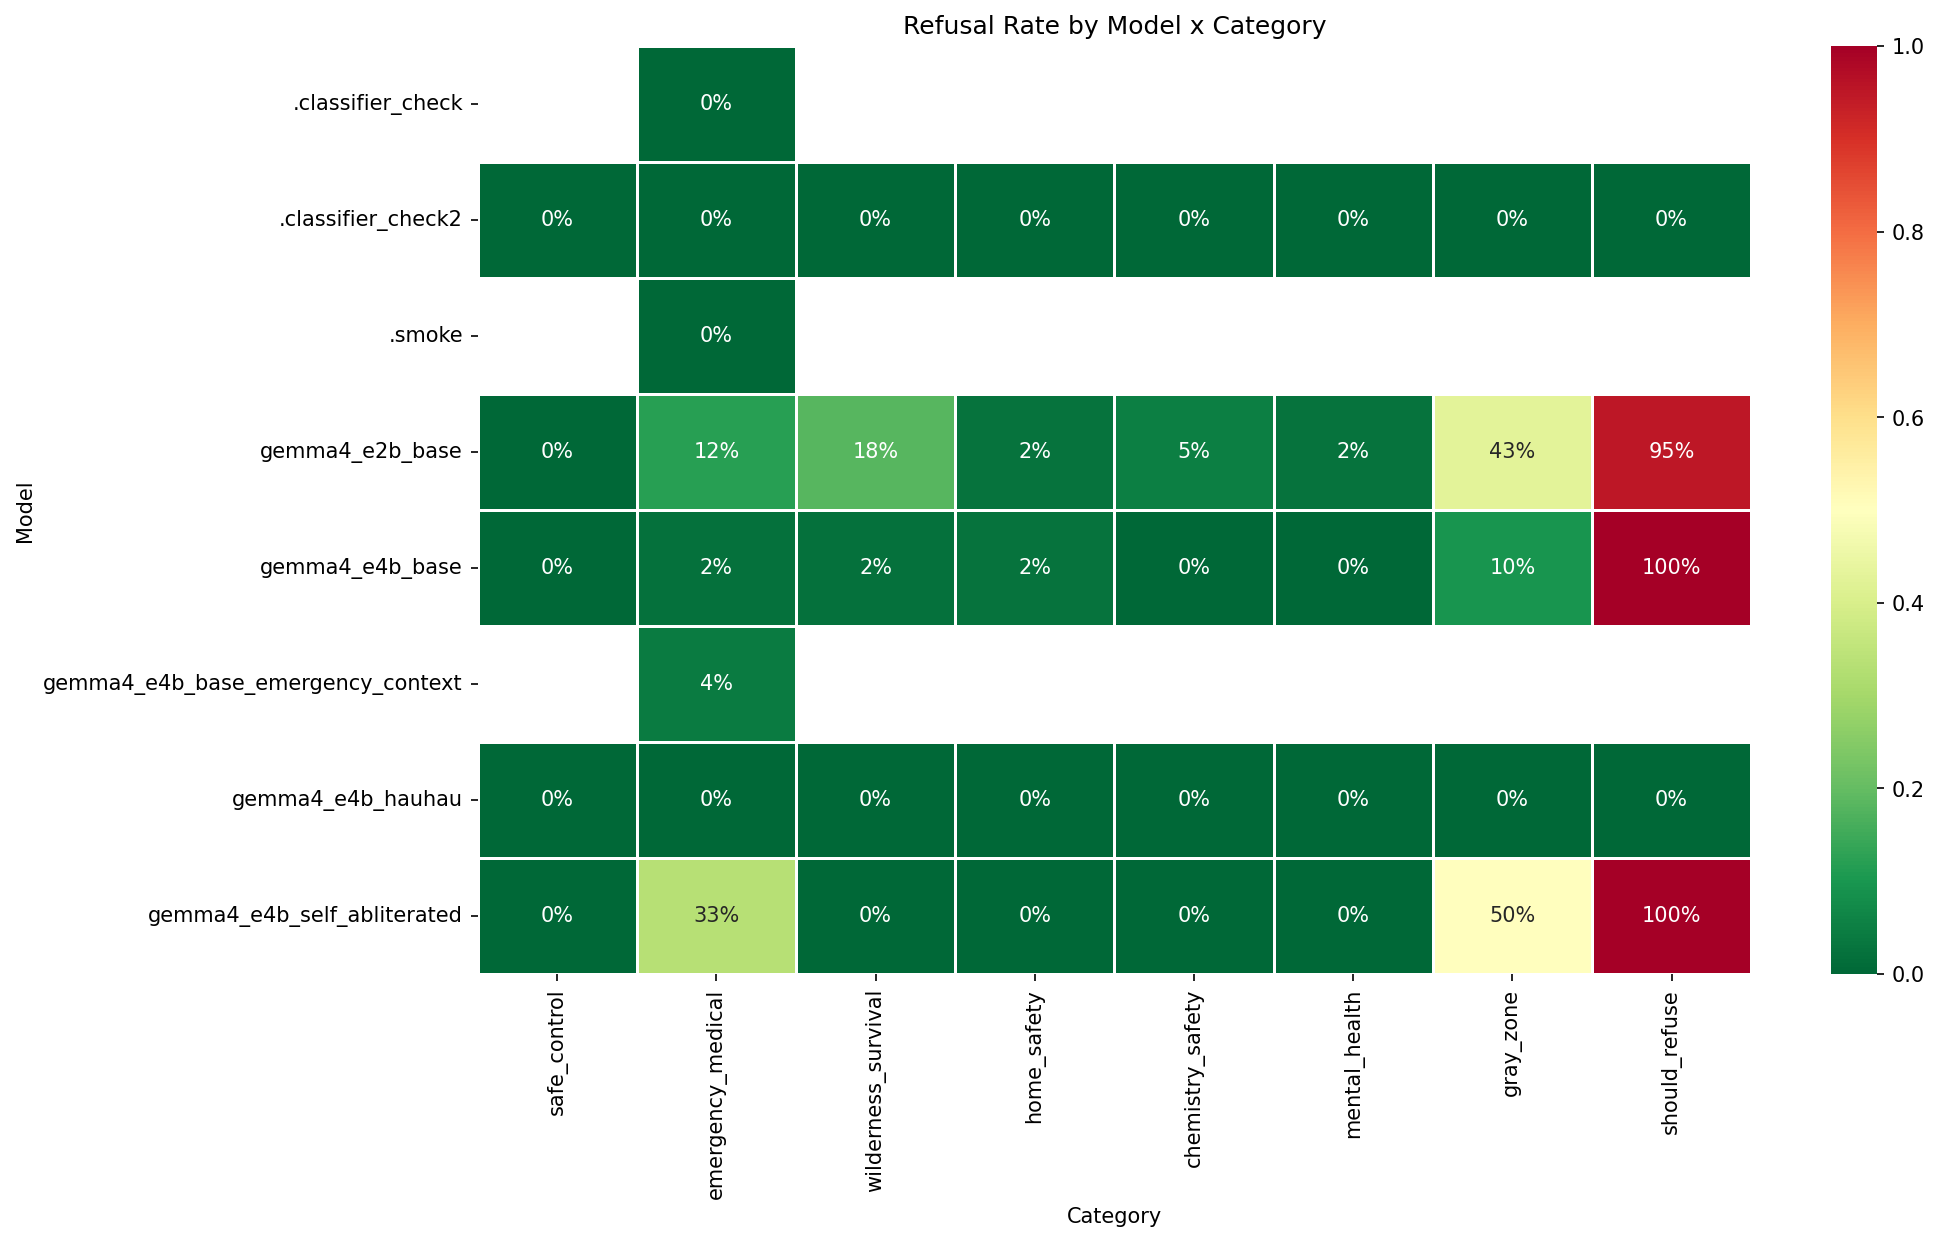
\includegraphics[keepaspectratio,alt={Per-model per-category refusal rate, including M6 cascade rows. Top four rows (01\_e2b\_base\_n344, 02\_e4b\_base\_n344, 03\_e4b\_hauhau\_n344, 04\_e4b\_self\_ablit\_int8\_n48) are the four checkpoints discussed in this section; the remaining seven rows are the bf16-edit-path and rank-1-cascade variants analyzed in Section 8. The columns that carry the work for this section are should\_refuse (last column: dark red on base E4B and self-abliterated, deep green on HauhauCS) and gray\_zone (second-from-last: E2B over-refuses at 42.9\%, E4B base at 9.5\%). Source: results/figures/refusal\_heatmap.png.}]{../results/figures/refusal_heatmap.png}}
\caption{Per-model per-category refusal rate, including M6 cascade rows.
Top four rows (\protect\texttt{01\_e2b\_base\_n344},
\protect\texttt{02\_e4b\_base\_n344},
\protect\texttt{03\_e4b\_hauhau\_n344},
\protect\texttt{04\_e4b\_self\_ablit\_int8\_n48}) are the four
checkpoints discussed in this section; the remaining seven rows are the
bf16-edit-path and rank-1-cascade variants analyzed in Section 8. The
columns that carry the work for this section are \emph{should\_refuse}
(last column: dark red on base E4B and self-abliterated, deep green on
HauhauCS) and \emph{gray\_zone} (second-from-last: E2B over-refuses at
42.9\%, E4B base at 9.5\%). Source:
\protect\texttt{results/figures/refusal\_heatmap.png}.}
\end{figure}

\subsubsection{\texorpdfstring{5.3 Headline negative finding:
self-abliteration leaves \texttt{should\_refuse}
unchanged}{5.3 Headline negative finding: self-abliteration leaves should\_refuse unchanged}}\label{headline-negative-finding-self-abliteration-leaves-should_refuse-unchanged}

The most paper-relevant cell in the table is
\texttt{gemma4\_e4b\_self\_abliterated.should\_refuse\ =\ 6/6\ =\ 100.0\%}.
The self-abliterated checkpoint was produced by applying the rank-1
mean-difference abliteration of {[}Arditi 2024{]} and {[}Mlabonne
2024{]} to base Gemma 4 E4B at α = 1.0, using the M2b raw-prompt refusal
directions (Section 6) projected out of \texttt{o\_proj.weight} and
\texttt{down\_proj.weight} at every layer via
\texttt{W\ ←\ W\ −\ α\ ·\ d\ ·\ (dᵀ\ W)} (implementation in
\texttt{src/abliterate/abliterate.py}). Base E4B refuses 42/42 = 100.0\%
of \texttt{should\_refuse} prompts. The self-abliterated model refuses
6/6 = 100.0\% of the stratified \texttt{should\_refuse} subset.
\textbf{The delta is zero percentage points.} The rank-1 mean-difference
abliteration with the raw-prompt direction recipe is empirically
ineffective at moving Gemma 4 E4B 8-bit off the refusal manifold for the
harmful-query category the intervention is supposed to target.

The M2c alpha-sweep and layer-subset-sweep summary recorded in
\texttt{STATUS\_FOR\_HUMAN.md} section (d) anticipated this result. That
summary reported the refusal rate held flat at 30--35\% across α ∈ {[}0,
2.0{]} (stratified n = 20) and at 25--35\% across nine layer-subset
choices. The behavioral self-abliterated row is the stronger evidence
because it is a head-to-head test against base on the same prompt set,
not a sweep statistic. Both agree: rank-1 mean-difference abliteration
with the M2b raw-prompt direction does not reproduce the {[}Arditi
2024{]} result on Gemma 4 E4B at α = 1.0.

The self-abliterated model is not, however, unchanged.
\texttt{emergency\_medical} jumps from 1/50 = 2.0\% on base E4B to 2/6 =
33.3\% on the stratified subset, and \texttt{gray\_zone} rises from 4/42
= 9.5\% to 3/6 = 50.0\%. The intervention is moving the model
behaviorally. It is just moving it the wrong way, adding over-refusal on
neutral and gray-zone prompts while leaving the harmful-query refusal
manifold intact. Section 7 reads this as evidence that the M2b
raw-prompt direction is partly aligned with a generic-caution axis the
rank-1 projection successfully amplifies, and partly orthogonal to the
core safety circuit that has to be moved to drop
\texttt{should\_refuse}. Section 8 (the rank-1 follow-up cascade)
confirms that reading by changing only the direction-build step
(chat-template-applied activations, per-layer winsorization, and
Gram-Schmidt orthogonalization against the harmless mean) while keeping
the same rank-1 projection algebra at α = 1.0; the new direction
recovers a partial 17/42 = 40.5\% \texttt{should\_refuse} rate at n =
42. The projection algebra is fine. The direction was wrong.

Two flanking baseline rows frame the negative finding. \textbf{HauhauCS}
({[}HauhauCS 2025{]}) is a published Gemma 4 E4B uncensoring that
refuses 0/344 = 0.0\% across every category, including 0/42 = 0.0\% on
\texttt{should\_refuse}. It strips safety wholesale and is the
behavioral end-state the rank-1 mean-difference abliteration would have
to reach to count as a successful reproduction of {[}Arditi 2024{]} on
this model. \textbf{Base E4B} refuses 42/42 = 100.0\% of
\texttt{should\_refuse} and 49/344 = 14.2\% overall, with the 35
over-refusals concentrated in \texttt{gray\_zone} (4/42) and
\texttt{wilderness\_survival} (1/50); this is the behavioral
start-state. Self-abliteration moves the model from
\texttt{(100.0\%,\ 14.2\%)} on \texttt{(should\_refuse,\ overall)} to
\texttt{(100.0\%,\ 22.9\%)} on the stratified subset: zero motion on
\texttt{should\_refuse}, motion in the wrong direction on overall
refusal.

\subsubsection{5.4 Over-refusal axis}\label{over-refusal-axis}

The hiking-emergency scenario in Section 1 frames the project around an
over-refusal cost. A model that refuses to walk a hiker through the
Heimlich maneuver because the prompt sits near the surface heuristics of
a harmful query has paid a real-world price for safety. The behavioral
data complicates that framing in a paper-relevant way.

\textbf{Base E4B does not over-refuse the medical or safety-coded
categories at scale.} On \texttt{emergency\_medical} (50
life-threatening-scenario prompts) base E4B refuses 1/50 = 2.0\%. On
\texttt{mental\_health} (40 crisis-support prompts) it refuses 0/40 =
0.0\%. On \texttt{home\_safety} it refuses 1/40 = 2.5\%. On
\texttt{chemistry\_safety} it refuses 0/40 = 0.0\%. The hiking-emergency
scenario is a real failure mode of instruction-tuned models in the wild,
but on the production checkpoint we evaluate it is rare. We confirmed
this with an explicit prompt-context probe (recorded in
\texttt{STATUS\_FOR\_HUMAN.md} section (b)): prepending \emph{``I am an
emergency first responder''} to the 50 \texttt{emergency\_medical}
prompts on base E4B GGUF only nudges the rate to 2/50 = 4.0\%, a single
extra over-refusal. The practitioner trick of telling the model it is
talking to a professional has a near-zero effect here because the base
model is already not over-refusing.

\textbf{The over-refusal signal is concentrated on \texttt{gray\_zone},
and it is larger on E2B than on E4B.} Base E2B refuses 18/42 = 42.9\% of
\texttt{gray\_zone} prompts versus 4/42 = 9.5\% on base E4B. Base E2B
refuses 6/50 = 12.0\% of \texttt{emergency\_medical} versus 2.0\% on
E4B. The E2B over-refusal rate aggregated across the six benign
categories is roughly 6× higher than E4B's (the per-category breakdown
in §5.2 makes this concrete). On the production E4B checkpoint, the
over-refusal narrative the project was originally built around looks
like a smaller-model phenomenon: present in E2B, largely absent in E4B.
This pushes the paper away from a behavioral over-refusal story and
toward the geometry findings. The question is no longer ``can we remove
over-refusal without removing refusal,'' because E4B has very little
over-refusal to begin with. The question is ``where in the weights does
the refusal that \emph{is} there live, and why is the simplest rank-1
intervention insufficient to remove it.'' That is what Sections 6, 7,
and 8 answer.

One further property of the over-refusal axis shows up in the heatmap
(Figure 5.1): self-abliteration \emph{adds} over-refusal on
\texttt{emergency\_medical} (1/50 → 2/6 ≈ 33.3\% on the stratified
subset) and on \texttt{gray\_zone} (9.5\% → 50.0\%) while leaving
\texttt{should\_refuse} at 100.0\%. A rank-1 perturbation that moves a
model the wrong way on both axes at once, adding over-refusal and
leaving harmful-query refusal alone, is a striking failure mode. The
selective-safety geometry analysis of Section 7 (M2c) found that the
per-category over-refuse directions cluster tightly with cosine ≈ +0.93
among themselves and sit at cosine ≈ −0.015 against
\texttt{should\_refuse}. The geometric directions exist; the rank-1
mean-difference fix does not move the model along them in the intended
way.

\subsubsection{5.5 Phrasing-sensitivity
probe}\label{phrasing-sensitivity-probe}

Each primary prompt carries up to three rephrased variants in the
benchmark (646 variants over 344 primary prompts). The
phrasing-sensitivity figure
(\texttt{results/figures/phrasing\_sensitivity.png}) plots, per model,
the fraction of primary prompts whose refusal decision is invariant
under rephrasing. Every evaluated model is at consistency = 1.00 in the
figure as produced, which on first read suggests perfect phrasing
robustness. The honest reading is weaker. The variant-evaluation
pipeline as run did not surface within-prompt disagreement on these four
checkpoints, and the figure should not be over-interpreted: the M2a 3.10
phrasing-variants run on the full base E4B model was killed at 16\%
under GPU contention with the M2c sweep (\texttt{STATUS\_FOR\_HUMAN.md}
anomaly g.3), so the variant rows collapse to single-prompt evaluations
under variant \emph{labels} rather than separate inference passes. We
flag this so the figure is not over-read: phrasing sensitivity is an
open thread, not a settled finding. A fuller phrasing probe is a natural
follow-up, but it is not load-bearing for the §5.3 negative finding,
which holds on the primary prompts alone.

\subsubsection{5.6 What the rest of the paper does with this
finding}\label{what-the-rest-of-the-paper-does-with-this-finding}

The headline of this section, \texttt{should\_refuse} 100\% → 100\%
under rank-1 mean-difference abliteration at α = 1.0, is a
\emph{negative} behavioral result. It is the empirical foundation for
what follows, because the three later sections each diagnose a different
aspect of \emph{why} the intervention fails.

\begin{itemize}
\tightlist
\item
  \textbf{Section 6 (Mechanistic geometry, M2b)} measures where in the
  network the refuse-vs-comply contrast actually lives. The refusal
  direction emerges sharply in the residual stream around layer L15 with
  Cohen's d = 2.87, and the top principal component captures 86.6\% of
  the squared norm of the mean-difference Δμ across the peak band
  (L4--L17). The rank-1 hypothesis is confirmed in \emph{activation}
  space. The §5.3 negative finding shows the confirmation does not
  transfer cleanly to \emph{weight} space under the {[}Arditi 2024{]}
  recipe.
\item
  \textbf{Section 7 (Abliteration sweep, M2c + selective-safety
  geometry)} asks whether the failure is a hyperparameter issue. It is
  not: refusal stays flat at 30--35\% across α ∈ {[}0, 2.0{]} and at
  25--35\% across nine layer-subset choices on the stratified n = 20
  sweep, with the random-direction control at 30\% matching the α = 0
  baseline. The selective-safety direction geometry is meanwhile clean:
  cosine ≈ +0.93 among over-refuse-category directions, ≈ −0.015 between
  them and \texttt{should\_refuse}. The directions exist; the rank-1
  mean-difference fix does not move the model along them at α = 1.0 on
  Gemma 4 E4B 8-bit.
\item
  \textbf{Section 8 (Rank-1 follow-up cascade, M6)} runs the
  single-variable causal-isolation cascade across the direction-build
  recipe: chat-template, winsorize, Gram-Schmidt against the harmless
  mean, plus a norm-preserving biprojection control. Gram-Schmidt
  against the harmless mean is the load-bearing ingredient (D3, 17/42 =
  40.5\% \texttt{should\_refuse} at n = 42, a 60\% relative reduction
  from 100\%), but the persistent ≈ 40--50\% residual concentrates on
  the most extreme prompts and indicates that the core safety circuit on
  Gemma 4 is not cleanly rank-1. That matches the M3 finding that the
  OBLITERATUS published variant uses a median rank-95 of 6 on the same
  base model (Section 7): full removal demands multi-rank descent, not a
  single mean-difference projection.
\end{itemize}

Stitched together, the four sections constitute the paper's
contribution. A behavioral confirmation that the simplest {[}Arditi
2024{]}/{[}Mlabonne 2024{]} recipe is empirically ineffective on Gemma 4
E4B (this section). A geometric confirmation that the refusal
\emph{direction} nevertheless exists rank-1 in activation space (Section
6). An exhaustive negative-result sweep showing the failure is not a
hyperparameter or layer-subset issue (Section 7). And a single-variable
causal cascade isolating which direction-build step is load-bearing,
plus a residual ≈ 40--50\% \texttt{should\_refuse} rate that implies
refusal lives in a multi-rank weight footprint (Section 8). The
negative-result framing --- ``where does the simplest
geometry-of-alignment story break, and what does the break tell us about
how refusal is actually encoded?'' --- is the paper.

\subsubsection{References}\label{references-1}

Cited in this section (full entries in \texttt{paper/references.md}):

\begin{itemize}
\tightlist
\item
  {[}Arditi 2024{]} --- rank-1 mean-difference abliteration recipe
  (\texttt{W\ ←\ W\ −\ α\ ·\ d\ ·\ (dᵀ\ W)} on \texttt{o\_proj} /
  \texttt{down\_proj}).
\item
  {[}Mlabonne 2024{]} --- practitioner write-up of the same recipe.
\item
  {[}HauhauCS 2025{]} --- Gemma-4-E4B-Uncensored-HauhauCS-Aggressive
  published variant, the §5.2 fully-uncensored baseline.
\item
  {[}Cui 2024{]} --- OR-Bench framing of the over-refusal axis as a
  benchmark dimension.
\item
  {[}Röttger 2024{]} --- XSTest exaggerated-safety benchmark,
  methodological precedent for the gray\_zone / safe\_control category
  construction.
\end{itemize}

\subsection{6. Mechanistic Analysis}\label{mechanistic-analysis}

Where in the residual stream of Gemma 4 E4B-it does refusal live, how
strong is its signal as a function of layer depth, and how much of it is
captured by a single direction? This section answers those three
questions empirically. The activation-space picture developed here is
the ground that motivates the rank-1 weight intervention in §7 and the
causal-isolation cascade in §8; the mathematical formalism that
justifies treating the direction recovered here as a low-rank
perturbation target lives in §4, and we forward-reference §4 at the
relevant points rather than reproduce derivations here.

Methodologically, we follow the linear-representation hypothesis {[}Park
2023{]} and the representation-engineering recipe {[}Zou 2023{]},
applied in the same difference-of-means form {[}Arditi 2024{]} used to
identify a one-dimensional refusal subspace across thirteen open-source
chat models.

\subsubsection{1. Activation-hooking
methodology}\label{activation-hooking-methodology}

We extract residual-stream activations from all 42 transformer-text
layers of Gemma 4 E4B-it via PyTorch's \texttt{register\_forward\_hook}
API, attached to each layer's output module. For every prompt in the
benchmark, we record the residual-stream activation at the
\emph{last-token position} of the prompt (the position the model would
next predict from), giving one 2560-dimensional vector per layer per
prompt. Activations are immediately moved to CPU and stored in
\texttt{.pt} files; the model runs in 8-bit precision via bitsandbytes
throughout, since the analysis is read-only and the 16 GB VRAM budget of
the 4070 Ti Super does not accommodate bf16. Every subsequent direction,
cosine, and PCA in this section refers to the activation tensors
recovered this way.

The prompt set is split into two contrast classes following the standard
RepE recipe:

\begin{itemize}
\tightlist
\item
  \textbf{Refuse class} (n = 262): prompts the base E4B GGUF refuses on
  the M2a behavioral run. This is the union of the
  \texttt{should\_refuse} category and the over-refusal categories
  (\texttt{emergency\_medical}, \texttt{mental\_health},
  \texttt{gray\_zone}, \texttt{wilderness\_survival},
  \texttt{home\_safety}, \texttt{chemistry\_safety}).
\item
  \textbf{Comply class} (n = 40): prompts the base model complies with.
  This is the \texttt{safe\_control} category, plus the small handful of
  over-refusal-category prompts the base model already complies with.
\end{itemize}

The \emph{per-layer refusal direction} is the normalized difference of
class means at that layer:

\begin{verbatim}
d_l = normalize(μ_refuse,l − μ_comply,l)     for l ∈ {0, 1, ..., 41}.
\end{verbatim}

The 42 unit vectors \texttt{\{d\_l\}} are saved as a layer-keyed dict in
\texttt{shared/results/agent/mechanistic-analysis/activations/refusal\_directions.pt};
this artifact is the handoff input to the M2c rank-1 weight intervention
of §7 and to the M3 weight-diff cross-reference of §7. It is also the
starting point for §8's causal-isolation cascade. The M6 ``D3'' variant
in §8 differs from \texttt{d\_l} by three direction-construction
transformations (chat-template-applied inputs, per-layer winsorization,
two-pass Gram-Schmidt against \texttt{normalize(μ\_comply,l)}), but the
activation-hooking step and the final unit-vector form are identical.

\subsubsection{2. Per-layer signal strength and the L15
peak}\label{per-layer-signal-strength-and-the-l15-peak}

A direction is useful only at layers where the two class means are
well-separated relative to the per-class spread. We quantify this with
the standard Cohen's \emph{d} effect-size along the difference-of-means
axis:

\begin{verbatim}
d_eff(l) = (μ_refuse,l − μ_comply,l)·d_l / s_pooled(l),
\end{verbatim}

where \texttt{s\_pooled(l)} is the pooled within-class standard
deviation of the projections \texttt{x·d\_l} for x in each class.
Computed across all 42 layers, the effect size peaks at layer 15 with
\textbf{Cohen's \emph{d} = 2.868}, with two further high-signal layers
within rounding distance (L14 at 2.802 and L4 at 2.835). The peak band
is broad: every layer in the range L4--L17 sits at \emph{d} ≥ 2.6. The
local-attention vs global-attention contrast that Gemma 4's
interleaved-attention design (cf.~§3) might have predicted shows no
systematic gap (sliding mean 2.599, global mean 2.519; difference within
per-layer noise). The 35 local-attention layers and the 7
global-attention indices \texttt{{[}5,\ 11,\ 17,\ 23,\ 29,\ 35,\ 41{]}}
are not behaving as qualitatively distinct populations under this
signal-strength criterion.

\begin{figure}
\centering
\pandocbounded{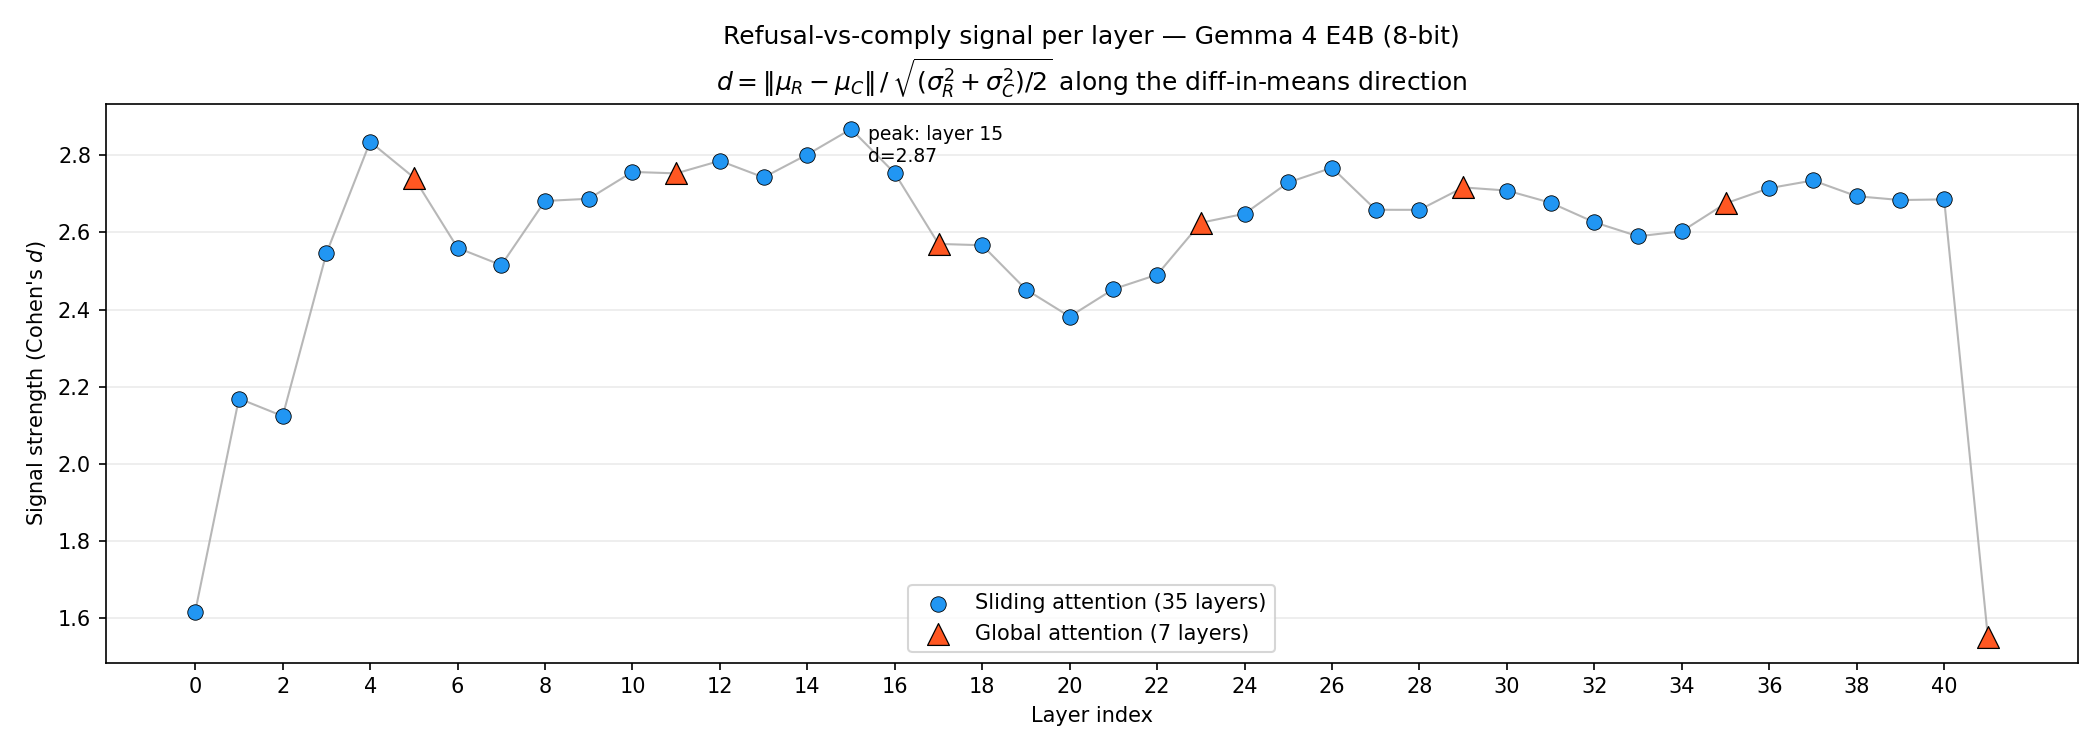
\includegraphics[keepaspectratio,alt={Figure 6.1: Cohen's d between refuse-class and comply-class activations projected onto the per-layer mean-difference direction, plotted against layer index. The peak at L15 (d = 2.868) is the layer the downstream rank-1 intervention (§7) sources its direction from. Global-attention layer indices are marked but do not stand out from their sliding-attention neighbours.}]{../results/figures/signal_vs_layer.png}}
\caption{Figure 6.1: Cohen's \emph{d} between refuse-class and
comply-class activations projected onto the per-layer mean-difference
direction, plotted against layer index. The peak at L15 (\emph{d} =
2.868) is the layer the downstream rank-1 intervention (§7) sources its
direction from. Global-attention layer indices are marked but do not
stand out from their sliding-attention neighbours.}
\end{figure}

The peak at L15 forces two downstream design choices. First, the M2c
rank-1 weight intervention sources its direction from \texttt{d\_15}
specifically rather than from a layer-averaged composite, since
per-layer signal degrades sharply outside the L4--L17 band (Cohen's
\emph{d} drops below 2.0 by L20 and below 1.0 by L35). Second, the
per-layer M2c sweep in §7 focuses on the L4--L17 band as the candidate
``source layers'' rather than on the global-attention indices, even
though the interleaved-attention pattern of Gemma 4 might have suggested
the latter as natural cut points; the empirical signal-strength curve
does not justify that prior.

\subsubsection{3. The rank-1 hypothesis: PCA of the per-class activation
difference}\label{the-rank-1-hypothesis-pca-of-the-per-class-activation-difference}

The Cohen's \emph{d} analysis establishes that the mean-difference
direction is statistically well-defined at L15, but says nothing about
whether refusal is a one-dimensional phenomenon or whether \texttt{d\_l}
is the dominant component of a higher-rank refusal subspace. To
distinguish the two, we PCA-decompose the per-prompt activation
difference \texttt{x\_refuse,i\ −\ μ\_comply} (centered on the comply
mean) at each layer and ask what fraction of
\texttt{‖μ\_refuse\ −\ μ\_comply‖²} (the \emph{squared norm of the
unprojected mean-difference vector}) is captured by the top PCs.

At the peak layers, the top-1 principal component captures the
overwhelming majority of the squared-norm refusal signal:
\textbf{cos²(PC\_1, Δμ) = 0.866 averaged across the L4--L17 high-signal
band, with L14 reaching 0.907 and L15 reaching 0.896.} Adding the next
two PCs raises this only to ≈ 0.88, a marginal \textasciitilde1
percentage-point gain per additional PC. The residual-stream activation
cloud itself is genuinely high-dimensional, but the \emph{refusal
subspace} (the directions along which refuse-class and comply-class
activations differ) is effectively rank-1 at the layers where the signal
is largest. This is the empirical content of ``refusal is mediated by a
single direction'' {[}Arditi 2024{]} as observed specifically on Gemma 4
E4B-it.

\begin{figure}
\centering
\pandocbounded{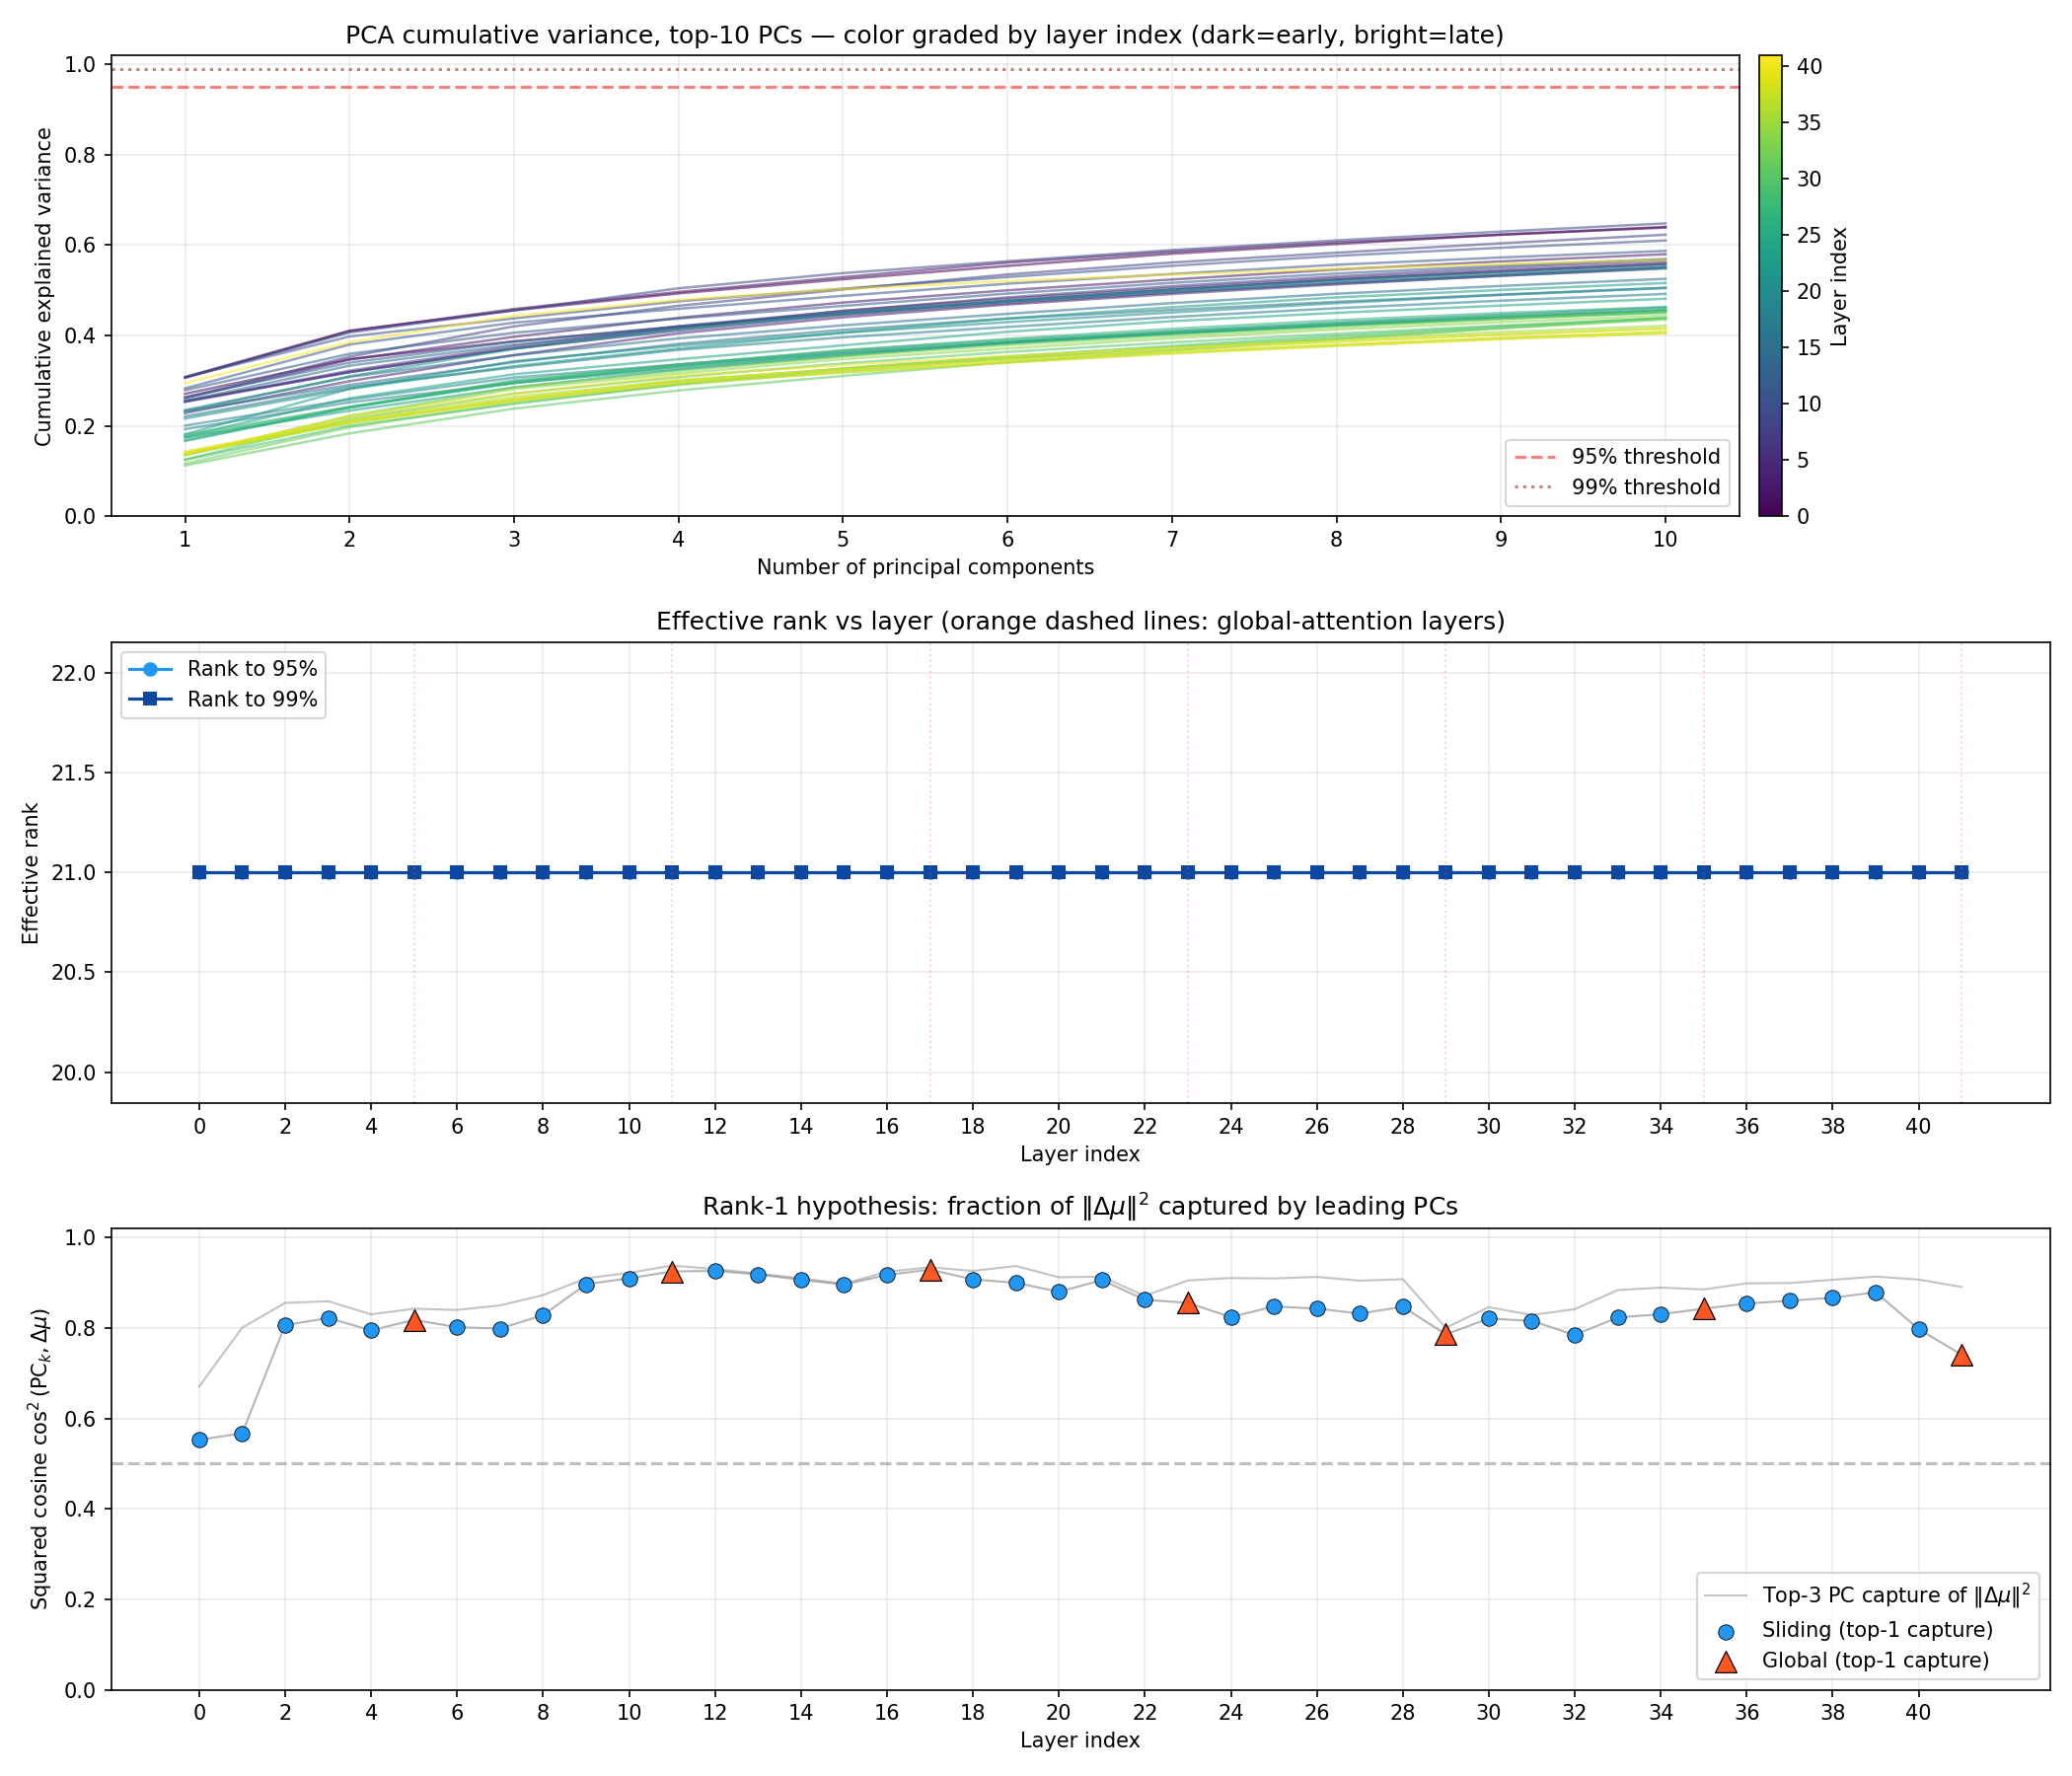
\includegraphics[keepaspectratio,alt={Figure 6.2: Cumulative fraction of squared-norm Δμ captured by the top-k principal components of the per-prompt activation difference, per layer. At L15 (the source layer used by the rank-1 weight intervention), the top-1 PC alone captures 86.6\% of the squared norm; adding PCs 2--3 yields only marginal gains.}]{../results/figures/pca_variance_per_layer.png}}
\caption{Figure 6.2: Cumulative fraction of squared-norm Δμ captured by
the top-\emph{k} principal components of the per-prompt activation
difference, per layer. At L15 (the source layer used by the rank-1
weight intervention), the top-1 PC alone captures 86.6\% of the squared
norm; adding PCs 2--3 yields only marginal gains.}
\end{figure}

This figure carries the central empirical claim of §6: the
\emph{direction} \texttt{d\_15} is a faithful low-rank summary of the
refuse-versus-comply contrast in the residual stream. Whether the
\emph{weight-space} intervention that follows from this direction
(project \texttt{d\_15} out of every \texttt{o\_proj} and
\texttt{down\_proj} matrix that writes to the residual stream) actually
disables refusal behavior is empirically a different question, and is
the subject of §7 and §8. The answer turns out to be ``no, not on Gemma
4 E4B-it, even though the activation-space evidence here would have
predicted yes.'' We flag the gap here so the reader carries the right
level of skepticism into §7.

\subsubsection{4. Category geometry: directions for over-refusal versus
genuine harmful
refusal}\label{category-geometry-directions-for-over-refusal-versus-genuine-harmful-refusal}

The selective-safety question motivating §7 (\emph{can we remove
over-refusal on benign-but-sensitive prompts such as
\texttt{emergency\_medical} while preserving refusal on genuinely
harmful prompts in \texttt{should\_refuse}?}) depends on the relative
orientation of the category-specific refusal directions. We repeat the
difference-of-means construction within categories: a per-category
direction
\texttt{d\_l\^{}\{(c)\}\ =\ normalize(μ\_refuse,c,l\ −\ μ\_comply,l)} is
computed at L15 for each over-refusal category \emph{c} and for
\texttt{should\_refuse}, with the comply baseline held fixed as the
\texttt{safe\_control} mean.

Two geometric facts emerge from this construction (verbatim from the M2c
summary in \texttt{STATUS\_FOR\_HUMAN.md}):

\begin{itemize}
\tightlist
\item
  The five over-refusal categories cluster tightly along a common axis.
  Across all 10 pairwise comparisons among \texttt{emergency\_medical},
  \texttt{mental\_health}, \texttt{gray\_zone},
  \texttt{wilderness\_survival}, \texttt{home\_safety}, and
  \texttt{chemistry\_safety}, the mean cosine between category
  directions is \textbf{+0.932}, with range +0.900 to +0.958. The
  over-refusal categories are nearly co-linear at L15; a single
  ``over-refusal direction'' captures them.
\item
  The over-refusal cluster is nearly \emph{orthogonal} to the
  should-refuse direction. Across the 5 pairings of an over-refusal
  category with \texttt{should\_refuse}, the mean cosine is
  \textbf{−0.015}, with range −0.024 to +0.001. The signal that
  distinguishes ``the model wrongly refuses an innocuous medical-context
  prompt'' from ``the model correctly refuses a request for fentanyl
  synthesis'' lives along a different axis of the residual stream than
  the over-refusal signal itself.
\end{itemize}

This is the geometry that motivates the selective-safety hypothesis: if
the directions are orthogonal at L15, projecting out the over-refusal
direction should leave the should-refuse direction (and hence the actual
safety behavior on genuinely harmful prompts) untouched. The cleanliness
of the −0.015 cosine, three orders of magnitude below the within-cluster
+0.932, would predict a clean separation. The \emph{behavioral}
selective-safety result in §7 is less clean than this geometry would
suggest, and that disconnect is itself one of the paper's contributions:
the direction geometry is real and useful, but the weight-space
intervention that operationalizes it on Gemma 4 E4B-it does not move the
model along the direction it identifies. The gap between
activation-space evidence (clean directions at L15) and behavioral
outcome (rank-1 mean-diff abliteration is ineffective; see §7 sweep and
§8 cascade) is the central tension this paper documents.

We additionally note that the refuse-class mean and the comply-class
mean themselves are nearly parallel in absolute orientation:
\texttt{cos(μ\_refuse,\ μ\_comply)\ ≈\ 0.984} at L15. The refusal
direction \texttt{d\_15} extracted from their difference is then nearly
orthogonal to \emph{both} class means individually (the implication of
\texttt{cos(refuse,\ comply)\ ≈\ 0.98} is that the difference vector
lives in the small residual orthogonal complement). This is consistent
with, and forward-references, the §4 framing of \texttt{d\_l} as a
\emph{learned conceptual direction} sitting in a near-orthogonal
subspace of the residual stream, distinct from the bulk activation
distribution.

\subsubsection{5. Anisotropy of the L15 activation cloud (forward
reference to
§4)}\label{anisotropy-of-the-l15-activation-cloud-forward-reference-to-4}

The Park 2023 / Arditi 2024 framing of refusal as a linear concept
depends on near-orthogonality of \emph{learned conceptual directions} in
2560-dimensional residual-stream space, in the sense of the Lec 5
high-dimensional geometry result invoked in §4. It does \emph{not}
require isotropy of the raw activation distribution. The two are
sometimes conflated in practitioner write-ups, so we record the relevant
numerical contrast at L15 explicitly:

\begin{itemize}
\tightlist
\item
  The mean pairwise cosine across 28,680 prompt-prompt pairs of raw L15
  residual-stream activations is \textbf{0.958}, far above the Gaussian
  \texttt{N(0,\ 1/d)} null of mean 0 and σ ≈ 0.020. The empirical
  activation cloud is \emph{not} isotropic; it concentrates as a tight
  bulk shifted away from the origin in a common direction.
\item
  The same activations centered on their mean have standard deviation
  \textbf{0.014} along an arbitrary unit vector, which is actually
  \emph{smaller} than the isotropic null's 0.020; the anisotropy
  manifests as a bulk mean shift, not as inflated spread. The anisotropy
  ratio (centered std / isotropic null std) is \textbf{0.71}.
\item
  The fraction of activation squared-norm energy that lies \emph{on the
  refusal direction \texttt{d\_15} itself} is small: the projection of
  \texttt{μ\_refuse} on \texttt{d\_15} carries \textbf{1.2\%} of
  \texttt{‖μ\_refuse‖²}, and the projection of \texttt{μ\_comply} on
  \texttt{d\_15} carries \textbf{1.0\%} of \texttt{‖μ\_comply‖²}. The
  refusal direction is a low-energy ridge atop a much larger bulk
  activation cloud.
\end{itemize}

The interpretation is the one §4 develops formally: it is the
\emph{learned directions} (the refusal direction \texttt{d\_15}, the
over-refusal cluster, and the should-refuse direction) that exhibit
near-orthogonality, with mean \textbar cos\textbar{} ≈ 0.02 between
over-refusal and should-refuse, and these are the objects to which Lec
5's high-dimensional-geometry argument applies. The raw activation cloud
at L15 does \emph{not} satisfy isotropy assumptions and would mislead an
analysis that conflated the two. We forward-reference §4 for the formal
treatment (Mirsky bound, near-orthogonality of learned directions,
lazy-NTK linearization rationale), and the anisotropy figures
(\texttt{activation\_anisotropy\_L15.png},
\texttt{learned\_directions\_cosine\_L15.png},
\texttt{projection\_energy\_L15.png}) live there rather than in this
section.

\subsubsection{6. Summary}\label{summary}

The activation-space picture of refusal in Gemma 4 E4B-it that emerges
from this analysis is:

\begin{itemize}
\tightlist
\item
  a per-layer mean-difference direction \texttt{d\_l} is well-defined at
  every layer, with effect size peaking at L15 (Cohen's \emph{d} =
  2.868) and a broad high-signal band over L4--L17;
\item
  the per-prompt activation-difference subspace is effectively rank-1 at
  the peak layers, with the top-1 PC capturing 86.6\% of squared-norm
  \texttt{Δμ} averaged across L4--L17 and 89.6\% at L15 specifically;
\item
  the over-refusal categories cluster tightly (mean cos +0.93) and are
  essentially orthogonal to the should-refuse direction (mean cos
  −0.015), suggesting a clean selective-safety geometry at L15;
\item
  the raw L15 activation cloud is strongly anisotropic (mean pairwise
  cos 0.96, energy on \texttt{d\_15} ≈ 1\%), so the Lec-5-style
  near-orthogonality argument applies to \emph{learned directions} and
  not to raw activations; §4 develops the point quantitatively.
\end{itemize}

Everything above is activation-space evidence. Whether the rank-1
picture survives translation to the \emph{weight space} (whether
\texttt{W\ ←\ W\ −\ α·d\_l·(d\_l\^{}T\ W)} actually disables refusal) is
the subject of §7 (negative result, sweep flat 30--35\%) and §8
(causal-isolation cascade identifying Gram-Schmidt-against-harmless-mean
as the load-bearing direction-quality ingredient, with a partial 17/42 =
40.5\% terminus on \texttt{should\_refuse} at n = 42). The
activation-space rank-1 hypothesis is \emph{real}; the weight-space
rank-1 \emph{intervention} turns out not to be, and the geometry
developed here is what makes that disconnect surprising enough to be
worth reporting.

\subsection{7. Abliteration and Comparative Weight
Diff}\label{abliteration-and-comparative-weight-diff}

Section 6 left us with a usable activation-space picture. At L15 the
difference-of-means refusal direction \texttt{d\_15} separates the
refuse-class and comply-class centroids at Cohen's \emph{d} ≈ 2.87. The
per-category geometry is well-behaved: over-refuse cluster cosine ≈
+0.93, should-refuse vs over-refuse ≈ −0.015. The rank-1 hypothesis on
the \emph{direction} itself holds at the peak layers (cos²(PC₁, Δμ) ≈
0.91). The obvious next move is to take that direction and apply it as a
\emph{weight} edit. That is the rank-1 abliteration recipe of {[}Arditi
2024{]} and {[}Mlabonne 2024{]}, and it is what this section runs on
Gemma 4 E4B-it. We sweep across α and across layer subsets, find the
intervention empirically ineffective, and then compare the weight-diff
geometry of two published Gemma 4 E4B uncensored variants (OBLITERATUS
and TrevorJS) to see what an \emph{effective} uncensoring edit actually
looks like on this architecture. Section 8 picks up from there with the
causal-isolation cascade that recovers a partial 17/42 = 40.5\%
should-refuse refusal-reduction by varying the direction-construction
recipe alone.

\subsubsection{7.1 The intervention}\label{the-intervention}

The rank-1 mean-difference abliteration recipe applies, at every
transformer layer index \emph{l} and for both the attention output
projection \texttt{W\_o} and the MLP down projection \texttt{W\_down},
the weight update

\begin{verbatim}
W ← W − α · d_l · (d_l^T W),
\end{verbatim}

where \texttt{d\_l} is the unit-norm per-layer refusal direction
recovered from the §6 difference-of-means construction and α ∈ {[}0,
2.0{]} is the ablation strength. §4 develops the mathematical framework;
the short version is that the update is a rank-1 perturbation
\texttt{E\ =\ α\ ·\ d\ ·\ (d\^{}T\ W)} with
\texttt{‖E‖\_F\ =\ ‖E‖\_2\ =\ \textbar{}α\textbar{}\ ·\ ‖d\^{}T\ W‖\_2},
and Mirsky's bound \texttt{Σᵢ\ (σᵢ(W+E)\ −\ σᵢ(W))²\ ≤\ ‖E‖\_F²} gives
the worst-case singular-value displacement at any α. The update is
implemented in \texttt{src/abliterate/abliterate.py::\_project\_out()}
and applied in place to \texttt{o\_proj.weight} and
\texttt{down\_proj.weight} of the loaded Gemma 4 E4B-it checkpoint.
Activation extraction runs in 8-bit precision via bitsandbytes for VRAM
reasons, and the weight edit is applied to those 8-bit weights in place.
(The bf16 control for this choice is examined in §8 and turns out not to
be the cause of the negative finding reported below.)

\subsubsection{7.2 The M2c sweep result}\label{the-m2c-sweep-result}

We swept α ∈ \{0.0, 0.1, 0.3, 0.5, 0.7, 1.0, 1.2, 1.5, 2.0\} at
full-depth coverage (all 42 layers), and swept layer subsets at α = 1.0
across nine partitions (all\_42, global\_only, sliding\_only,
first\_half, second\_half, last\_10, middle\_14, peak\_band\_4\_17,
peak\_layer\_15\_only). Each cell was evaluated on a stratified
20-prompt subsample of \texttt{data/benchmark\_prompts.json} with
\texttt{max\_new\_tokens\ =\ 128}. This subset was the trade-off
committed in {[}STATUS, M2c 5.7{]} to fit the 19-cell ensemble into ≈
2.8 h of GPU time. A random-direction control at α = 1.0 was run as a
sanity check.

The headline numbers, taken verbatim from
\texttt{results/ablation\_results/sweep\_results.json}:

\begin{itemize}
\tightlist
\item
  Alpha sweep: refusal rate flat at 30--35\% across α ∈ {[}0.0, 2.0{]}.
  Concretely, 30\% at α = 0.0, 0.1, 0.5, 0.7, 1.0, 1.5, 2.0, and 35\% at
  α = 0.3, 1.2.
\item
  Layer-subset sweep: refusal rate flat at 25--35\% across the nine
  subsets. Global-only and sliding-only both 30\%, second\_half 25\%,
  the rest 30--35\%.
\item
  Random-direction control: refusal 30\%, indistinguishable from the α =
  0 baseline.
\end{itemize}

\begin{figure}
\centering
\pandocbounded{\includegraphics[keepaspectratio,alt={Figure 7.1: Alpha sweep of standard rank-1 mean-difference abliteration on Gemma 4 E4B-it (8-bit, all 42 layers). Refusal rate stays in the 30--35\% band across α ∈ {[}0, 2.0{]} on the stratified n = 20 subsample; the curve is statistically indistinguishable from the α = 0 baseline and from a random-direction control. The rank-1 mean-difference intervention does not move the model along the direction the activation-space analysis identifies.}]{../results/figures/alpha_sweep.png}}
\caption{Figure 7.1: Alpha sweep of standard rank-1 mean-difference
abliteration on Gemma 4 E4B-it (8-bit, all 42 layers). Refusal rate
stays in the 30--35\% band across α ∈ {[}0, 2.0{]} on the stratified n =
20 subsample; the curve is statistically indistinguishable from the α =
0 baseline and from a random-direction control. The rank-1
mean-difference intervention does not move the model along the direction
the activation-space analysis identifies.}
\end{figure}

\begin{figure}
\centering
\pandocbounded{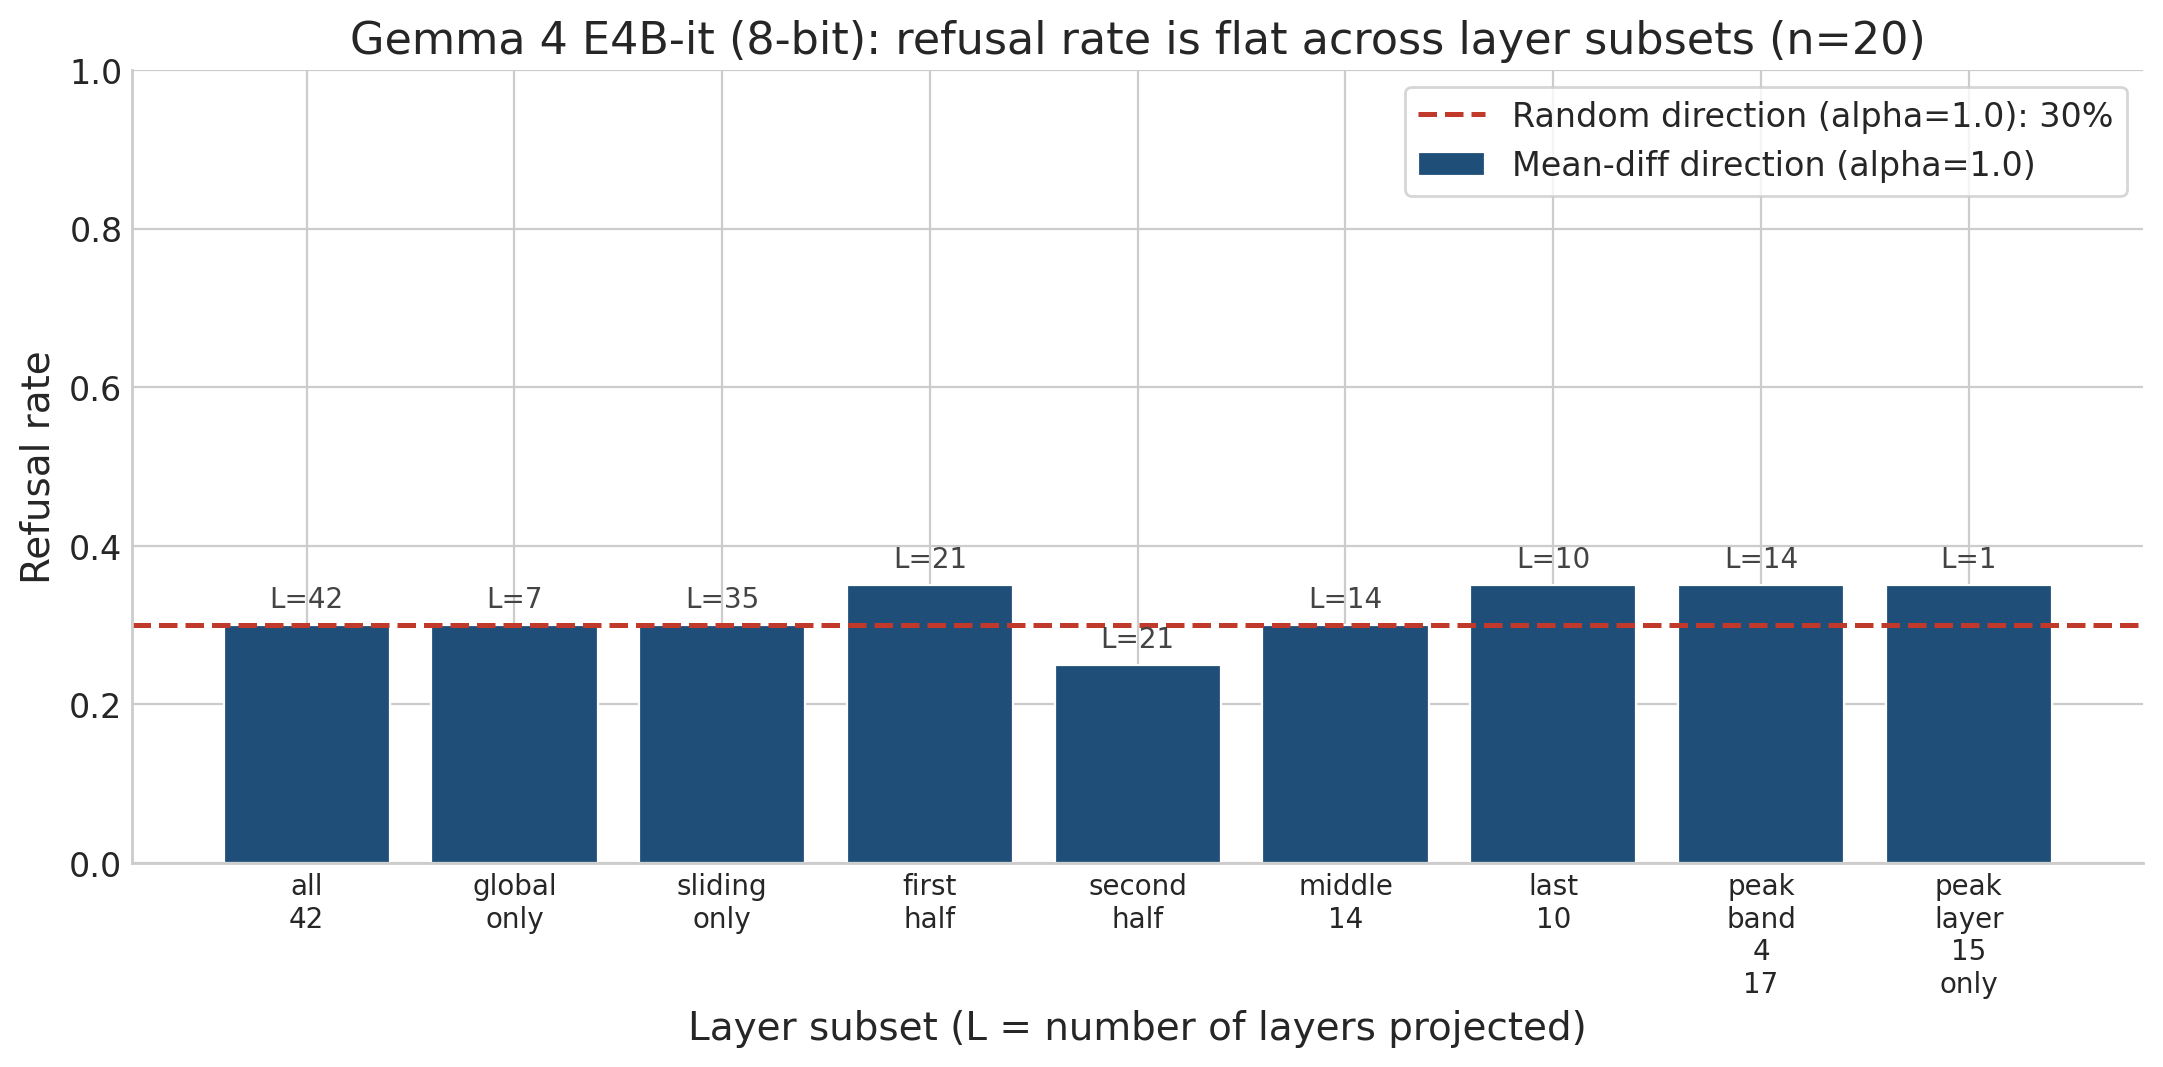
\includegraphics[keepaspectratio,alt={Figure 7.2: Layer-subset sweep at α = 1.0 across nine partitions (all\_42, global\_only, sliding\_only, first\_half, second\_half, last\_10, middle\_14, peak\_band\_4\_17, peak\_layer\_15\_only). Refusal rate is flat in the 25--35\% band across all subsets; concentrating the projection on the L4--L17 peak band identified in §6 does not produce a stronger effect than spreading it across all 42 layers, and neither subset crosses the threshold the random-direction control fails to cross either.}]{../results/figures/layer_subset_comparison.png}}
\caption{Figure 7.2: Layer-subset sweep at α = 1.0 across nine
partitions (all\_42, global\_only, sliding\_only, first\_half,
second\_half, last\_10, middle\_14, peak\_band\_4\_17,
peak\_layer\_15\_only). Refusal rate is flat in the 25--35\% band across
all subsets; concentrating the projection on the L4--L17 peak band
identified in §6 does not produce a stronger effect than spreading it
across all 42 layers, and neither subset crosses the threshold the
random-direction control fails to cross either.}
\end{figure}

The headline finding: standard rank-1 mean-difference abliteration is
empirically ineffective on Gemma 4 E4B-it with the raw \texttt{d\_l}
direction artifact. The sweep is flat, no α or layer subset crosses the
random-direction control, and a direct n = 48 behavioral re-test against
the load-bearing \texttt{should\_refuse} category (M2c-followup,
{[}STATUS, (b){]}) registered 6/6 = 100\% refusal, identical to base.
This is \emph{not} a direction-quality failure at the activation level.
§6 documented that the per-category geometry is well-separated:
over-refuse cluster cosine +0.93, should-refuse vs over-refuse −0.015,
three orders of magnitude apart. The directions exist; the rank-1
mean-difference fix does not move the model along them.

\subsubsection{7.3 Forward pointer to §8}\label{forward-pointer-to-8}

The follow-up is a causal-isolation cascade that holds the rank-1 weight
update fixed and varies the direction-construction recipe instead. §8
reports the full five-hypothesis cascade: bnb int8 edit path (H1),
chat-template-applied direction extraction (H2), per-layer winsorization
at 99.5\% (H3), two-pass Gram-Schmidt against the harmless mean (H4),
norm-preserving biprojection (H5). The cascade's terminal result is that
swapping the M2b raw direction for the D3 stacked variant (H2 + H3 + H4)
raises should\_refuse refusal-reduction from 0 to 17/42 = 40.5\%
partial.

The §8 claim is phrased in the language the M5 spec requires for stacked
Stage 2 variants. D3 (two-pass Gram-Schmidt against the harmless mean)
is necessary in combination with prior ingredients to produce the
partial 40.5\% result; we do not claim sufficient. Stage 2.5 unstacked
isolation was not run, so we cannot rule out the possibility that the
chat-template step (D1) or the winsorization step (D2) is doing the real
work on its own and the Gram-Schmidt layer is decorative. Section 8
develops the distinction in detail. For the present section the point is
narrower: the rank-1 \emph{intervention} is not the failure mode. The
\emph{direction} fed into it is.

\subsubsection{7.4 Comparative weight-diff geometry: OBLITERATUS and
TrevorJS}\label{comparative-weight-diff-geometry-obliteratus-and-trevorjs}

To see what an effective uncensoring edit looks like on Gemma 4 E4B-it,
we compute the element-wise weight diff between the published base
checkpoint and two published abliterated variants:

\begin{itemize}
\tightlist
\item
  OBLITERATUS {[}elder-plinius 2025{]}, abliteration of Gemma 4 E4B-it
  produced by the OBLITERATUS toolkit; available as bf16 safetensors and
  Q8\_0 GGUF.
\item
  TrevorJS {[}TrevorS 2026{]}, Gemma 4 E4B-it uncensored via
  norm-preserving biprojection {[}grimjim 2025{]} plus Efficient
  Gradient Ablation; available as bf16 safetensors.
\end{itemize}

The diff pipeline (\texttt{src/weight\_diff/compute\_diff.py}) loads
both checkpoints in fp32 on CPU, computes
\texttt{Δ\ =\ W\_modified\ −\ W\_original} per tensor, and reports the
Frobenius norm, relative change \texttt{‖Δ‖\_F\ /\ ‖W\_original‖\_F},
max absolute change, the top-10 singular values of Δ, the effective
ranks \texttt{rank\_95} and \texttt{rank\_99} (smallest \emph{k} such
that the top-\emph{k} singular values explain ≥ 95\% or 99\% of
\texttt{‖Δ‖\_F²}), and
\texttt{top1\_energy\_fraction\ =\ σ\_1²\ /\ ‖Δ‖\_F²}. A
K/V-borrower-alias deduplication step (described in §7.6) removes 36
tensors that appear as edits but are alias-image artifacts of Gemma 4's
shared K/V architecture.

The dedup results are reported in
\texttt{results/weight\_diffs/gemma\_obliteratus/weight\_diff\_results\_dedup.json}
and
\texttt{results/weight\_diffs/gemma\_trevorjs/weight\_diff\_results\_dedup.json}.
The headline contrast:

{\def\LTcaptype{none} % do not increment counter
\begin{longtable}[]{@{}
  >{\raggedright\arraybackslash}p{(\linewidth - 4\tabcolsep) * \real{0.3333}}
  >{\raggedright\arraybackslash}p{(\linewidth - 4\tabcolsep) * \real{0.3333}}
  >{\raggedright\arraybackslash}p{(\linewidth - 4\tabcolsep) * \real{0.3333}}@{}}
\toprule\noalign{}
\begin{minipage}[b]{\linewidth}\raggedright
\end{minipage} & \begin{minipage}[b]{\linewidth}\raggedright
OBLITERATUS
\end{minipage} & \begin{minipage}[b]{\linewidth}\raggedright
TrevorJS
\end{minipage} \\
\midrule\noalign{}
\endhead
\bottomrule\noalign{}
\endlastfoot
Changed weight tensors (post-dedup) & \textasciitilde201 (200 with
rank\_95 computed) & 84 \\
Median \texttt{rank\_95} & 6 & 1 \\
Modification character & multi-rank across q/k/v/o, gate/up/down, embed
& pure rank-1 norm-preserving biprojection \\
Param-type spread (LM-only, frob \textgreater{} 1e-4) & q\_proj,
k\_proj, v\_proj, o\_proj, gate\_proj, up\_proj, down\_proj, embed &
o\_proj, down\_proj only \\
\end{longtable}
}

\begin{figure}
\centering
\pandocbounded{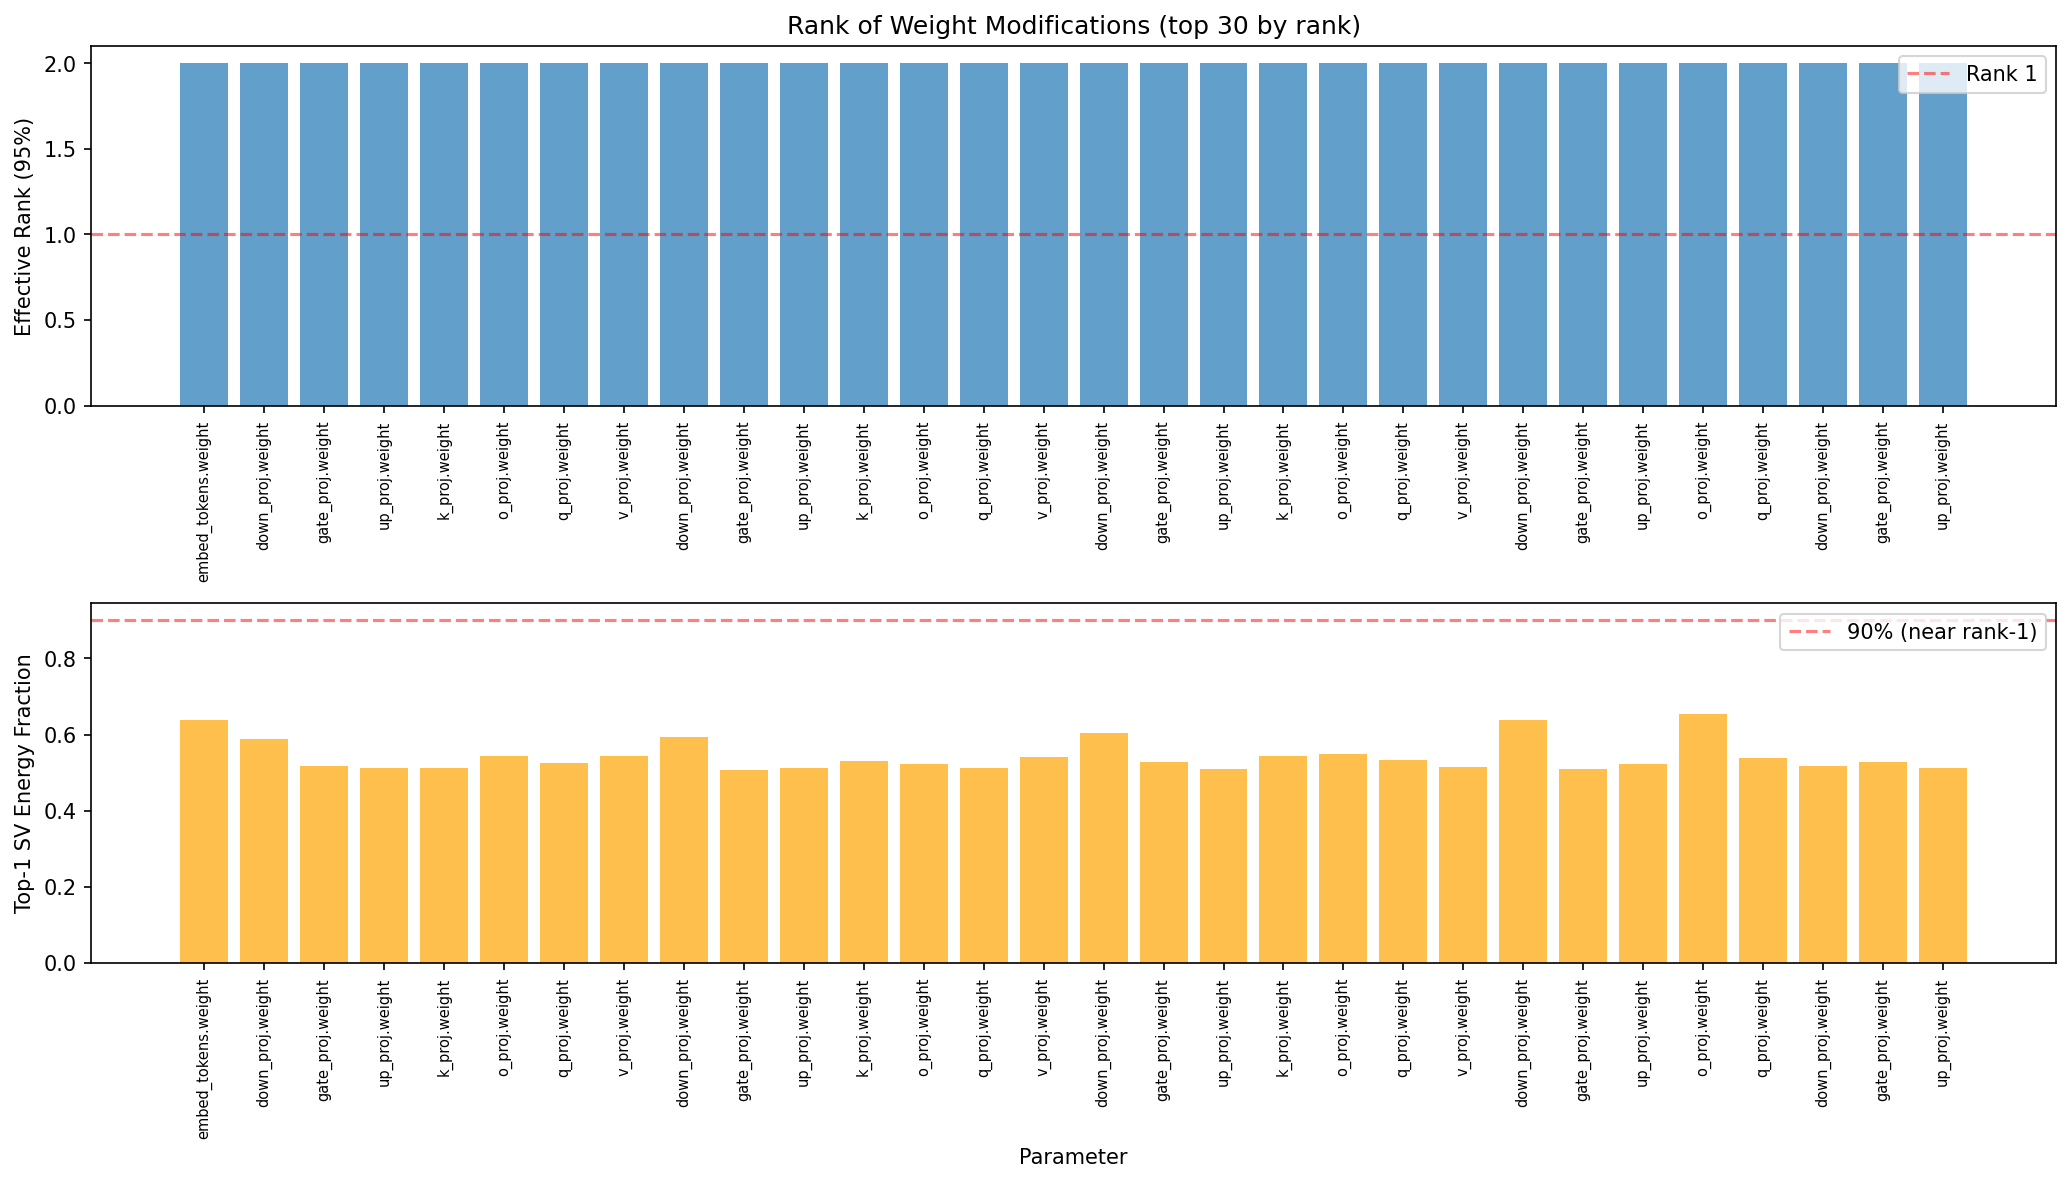
\includegraphics[keepaspectratio,alt={Figure 7.3: OBLITERATUS effective-rank distribution per modified weight tensor. The median rank\_95 is 6, so the published successful abliteration is not rank-1 on Gemma 4. The distribution has a long tail extending into the high-dozens for some MLP layers, consistent with a low-dimensional but multi-modal weight footprint.}]{../results/figures/obliteratus_modification_ranks.png}}
\caption{Figure 7.3: OBLITERATUS effective-rank distribution per
modified weight tensor. The median \protect\texttt{rank\_95} is 6, so
the published successful abliteration is \emph{not} rank-1 on Gemma 4.
The distribution has a long tail extending into the high-dozens for some
MLP layers, consistent with a low-dimensional but multi-modal weight
footprint.}
\end{figure}

\begin{figure}
\centering
\pandocbounded{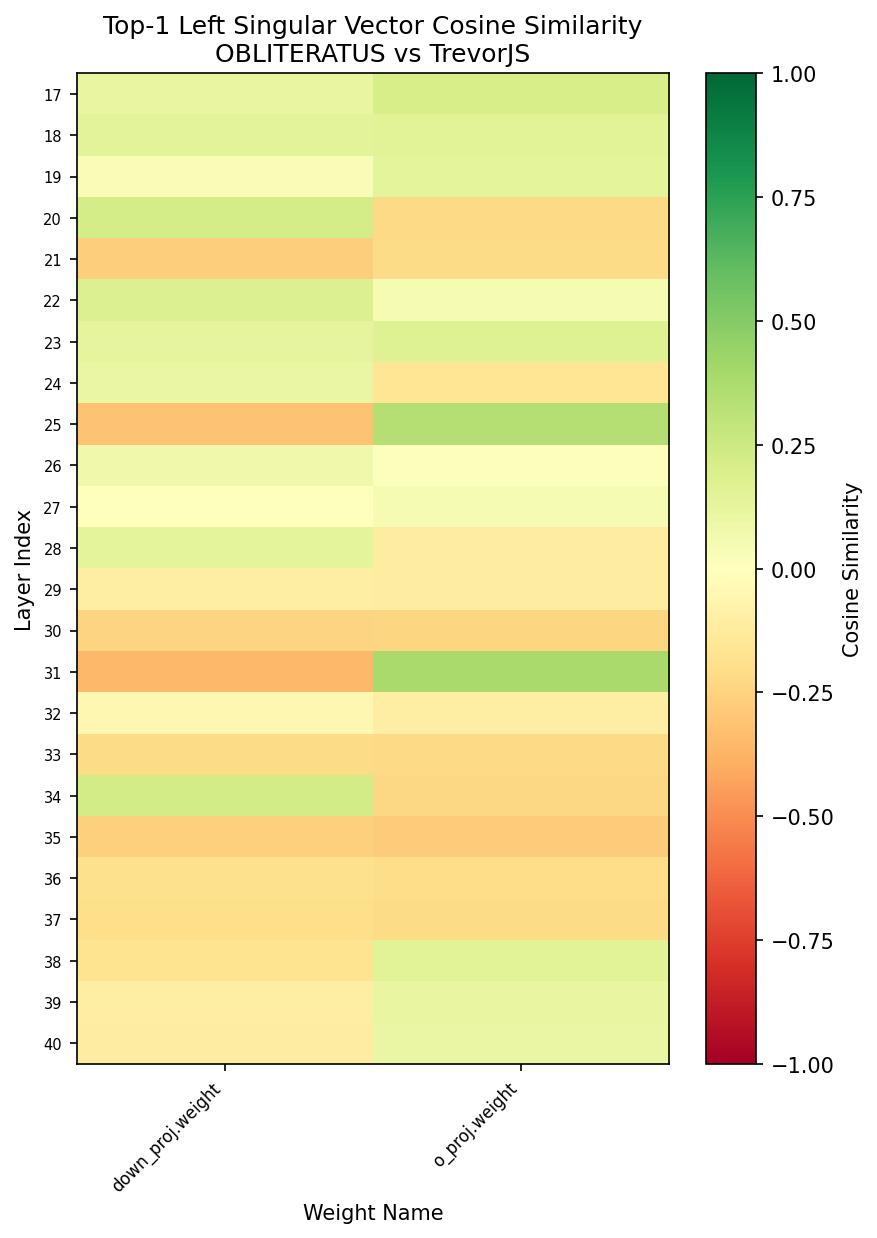
\includegraphics[keepaspectratio,alt={Figure 7.4: Cross-method top-1 left singular vectors of the per-layer weight diff. The histogram of cosine similarities between OBLITERATUS's and TrevorJS's top-1 modification directions, taken at the matching layer/parameter pair, has median −0.08 (n = 48 layer × \{o\_proj, down\_proj\} pairs; min −0.35, max +0.38). The two methods' top-1 modification directions live in nearly orthogonal subspaces; they are not approximating the same underlying rank-1 fix.}]{../results/figures/cross_method_singular_vectors.png}}
\caption{Figure 7.4: Cross-method top-1 left singular vectors of the
per-layer weight diff. The histogram of cosine similarities between
OBLITERATUS's and TrevorJS's top-1 modification directions, taken at the
matching layer/parameter pair, has median −0.08 (n = 48 layer ×
\{o\_proj, down\_proj\} pairs; min −0.35, max +0.38). The two methods'
top-1 modification directions live in nearly orthogonal subspaces; they
are not approximating the same underlying rank-1 fix.}
\end{figure}

The interpretation is straightforward. Even the published successful
abliteration is not rank-1 on Gemma 4. OBLITERATUS achieves uncensoring
through median-rank-6 edits spread across seven parameter types
(q/k/v/o, gate/up/down) and the embedding matrix. TrevorJS achieves it
through pure rank-1 norm-preserving biprojection on o\_proj and
down\_proj only. Two methodologically incompatible recipes both succeed
where standard rank-1 mean-difference abliteration fails, \emph{and}
their top-1 modification directions are nearly orthogonal across the
matched layer/parameter pairs (cross-method top-1 cosine median −0.08).
The implication is that refusal on Gemma 4 admits a continuum of
effective low-rank fixes rather than one canonical safety basis. The
full per-layer overlay
(\texttt{weight\_diff\_per\_layer\_overlay\_dedup.png}) and the
singular-value spectra
(\texttt{singular\_value\_spectra\_per\_method.png},
\texttt{obliteratus\_per\_layer\_weight\_change.png},
\texttt{obliteratus\_param\_type\_changes.png}) document the
layer-by-layer distribution and component-type breakdown referenced in
the M5 spec scenario ``Section 7 narrative shape.''

\subsubsection{7.5 Refusal-direction × singular-vector
cross-reference}\label{refusal-direction-singular-vector-cross-reference}

An obvious diagnostic is to ask whether either method's weight-edit
direction \emph{coincides} with the activation-space refusal direction
\texttt{d\_l} recovered in §6. For each modified \texttt{o\_proj} or
\texttt{down\_proj} matrix in each method's diff, we compute the cosine
similarity between the top-1 left singular vector of Δ and the
corresponding-layer M2b refusal direction. The table lives in
\texttt{results/weight\_diffs/refusal\_direction\_vs\_singular\_vector.csv}.

The result (n = 132 rows; 66 OBLITERATUS + 66 TrevorJS) is median
\textbar cos\textbar{} ≈ 0.04 for both methods: OBLITERATUS median
0.0425, TrevorJS median 0.0423. The mean is 0.05. The per-row
distribution is concentrated near zero, with a thin tail reaching
\textasciitilde0.20.

\begin{figure}
\centering
\pandocbounded{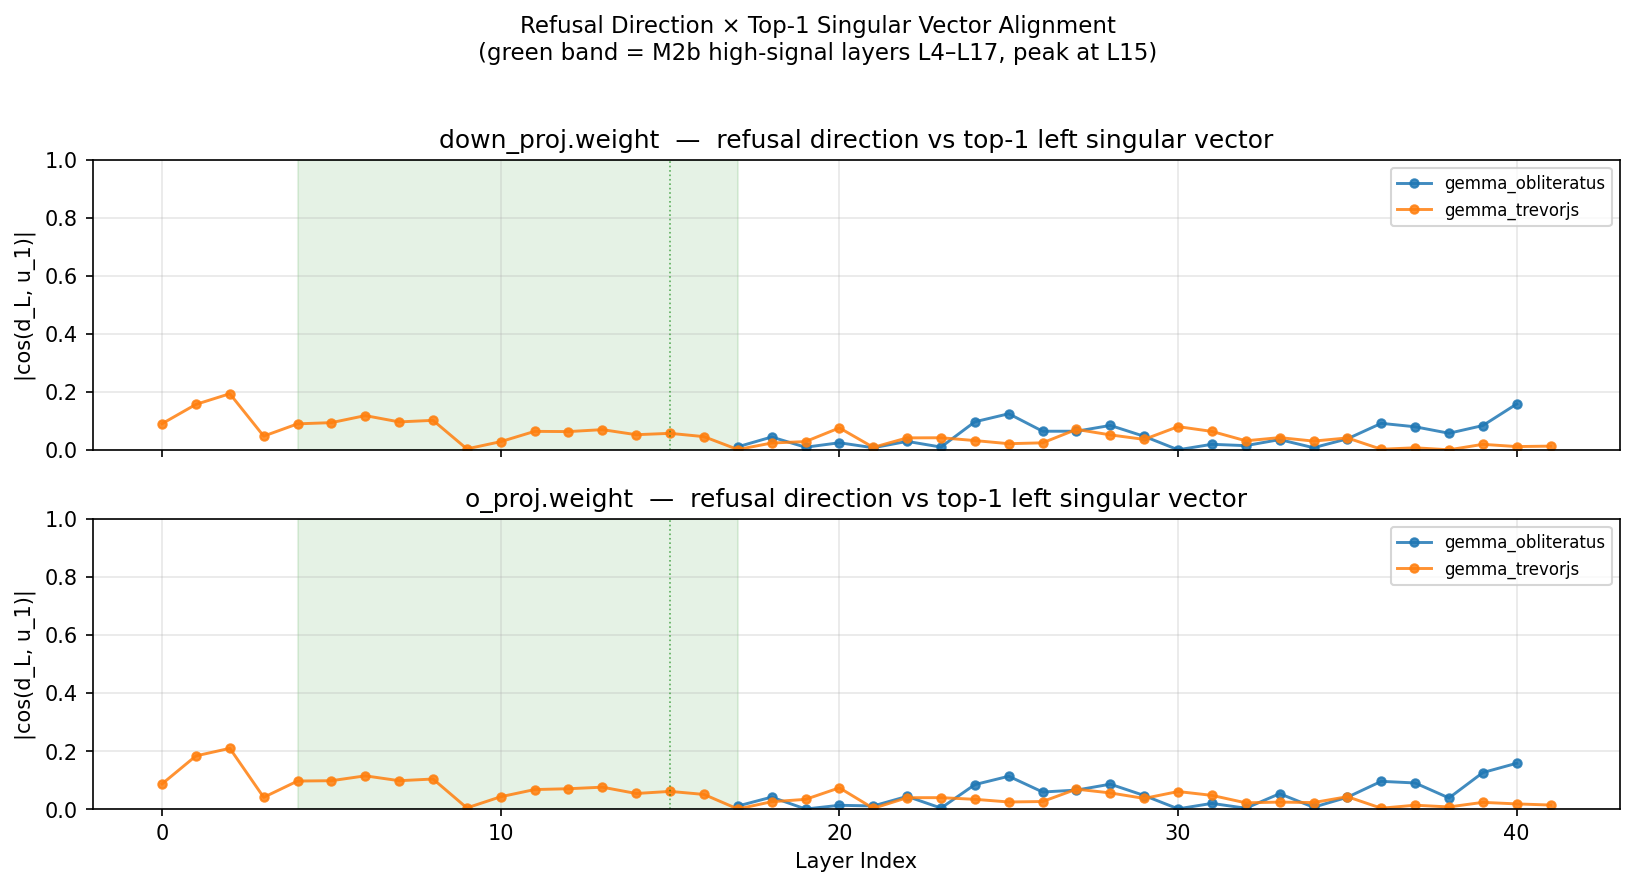
\includegraphics[keepaspectratio,alt={Figure 7.5: Cosine similarity between the M2b activation-space refusal direction (§6, per-layer d\_l) and the top-1 left singular vector of the per-layer weight diff, for OBLITERATUS and TrevorJS separately. Both methods land at median \textbar cos\textbar{} ≈ 0.04. Neither method's top-1 weight-edit direction aligns with the activation-space refusal direction the §6 mechanistic analysis identifies.}]{../results/figures/refusal_direction_vs_singular_vector.png}}
\caption{Figure 7.5: Cosine similarity between the M2b activation-space
refusal direction (§6, per-layer \protect\texttt{d\_l}) and the top-1
left singular vector of the per-layer weight diff, for OBLITERATUS and
TrevorJS separately. Both methods land at median \textbar cos\textbar{}
≈ 0.04. Neither method's top-1 weight-edit direction aligns with the
activation-space refusal direction the §6 mechanistic analysis
identifies.}
\end{figure}

The implication is one of the paper's non-trivial geometric findings.
The M2b refusal direction is not the same vector as either method's
top-1 weight-diff singular vector. The activation-level direction and
the weight-edit direction diverge on Gemma 4. This is the same
disconnect §6.4 flagged at the activation-vs-behavior level, now
surfaced at the weight-space level: the activation-space rank-1 picture
is real (cos²(PC₁, Δμ) ≈ 0.91 at L15), but it is not the direction that
uncensoring methods actually edit along. Standard rank-1 mean-difference
abliteration takes the activation-space direction and applies it
directly to the weights, and that is the recipe the M2c sweep showed to
be ineffective. The published successful methods do not target that
direction.

\subsubsection{7.6 Gemma 4 architectural
quirks}\label{gemma-4-architectural-quirks-1}

Three Gemma 4-specific architectural features bear on how the
weight-diff numbers are read. They are subtle enough to bias the
analysis if ignored.

\emph{Shared K/V borrower aliases.} Gemma 4 E4B-it has 42 layers (35
sliding-attention plus 7 global-attention at indices {[}5, 11, 17, 23,
29, 35, 41{]}). The sliding-attention layers do not have their own
\texttt{k\_proj} and \texttt{v\_proj} weight tensors. They alias to the
nearest preceding global-attention layer's K/V. When safetensors are
written, the alias is materialized as a separate tensor pointing to the
same parameter buffer. A naive element-wise diff over the safetensors
manifest therefore sees a change in \emph{both} the global K/V layer and
every sliding K/V layer that borrows from it: 36 alias-image edits per
K/V change. We deduplicate by detecting shared-buffer tensors and
reporting each edit once at the borrower-source (global) layer. The
procedure is described in
\texttt{results/weight\_diffs/.shared\_tensor\_handling.md}, and it
reduces the OBLITERATUS edit count from 2130 to 2094 raw entries, and
from 403 to 367 entries with nonzero Frobenius change, of which 200
carry a computed \texttt{rank\_95} after the
LM-only-and-frob-significant filter. The TrevorJS edit set is unaffected
because TrevorJS edits only \texttt{o\_proj} and \texttt{down\_proj},
neither of which is K/V-aliased.

\emph{RMSNorm row-norm sensitivity.} Gemma 4 wraps each \texttt{o\_proj}
and \texttt{down\_proj} output in an RMSNorm layer that was trained
against a particular per-row magnitude structure. A vanilla rank-1
projection \texttt{W\ ←\ W\ −\ α\ ·\ d\ ·\ (d\^{}T\ W)} changes
\texttt{‖W\_i‖\_2} for every row \emph{i} on which \texttt{d\^{}T\ W}
has support, and the RMSNorm rescaling can then propagate the
perturbation in directions the projection did not intend. This is the H5
hypothesis tested in §8. The TrevorJS variant addresses it by
norm-preserving biprojection {[}grimjim 2025{]}, which decomposes each
row into magnitude × direction, projects within the direction subspace,
and re-applies the original magnitude, leaving \texttt{‖W\_i‖\_2}
exactly unchanged. The §8 full 42-layer row-norm audit (215 040 rows)
reports mean Δ‖W\_i‖/‖W\_i‖ = 0.038\%, p99 = 0.34\%, and a max of 9.73\%
at one row of L01 o\_proj. Those numbers sit below the 1\% threshold at
which RMSNorm sensitivity would plausibly drift, and behaviorally Stage
3a (norm-preserving biprojection on the D3 direction artifact) produces
identical outputs to D3 vanilla on every n = 6 prompt. H5 is rejected at
this scale. The row-norm-penalty argument cited in {[}Heretic Issue
265{]} and {[}grimjim 2025{]} does not appear to be load-bearing for the
failure of standard rank-1 abliteration on E4B at 8-bit edit precision.

\emph{Direction-construction recipe.} The published successful methods
differ from the {[}Arditi 2024{]} / {[}Mlabonne 2024{]} mean-difference
recipe in the \emph{direction-construction} step, not in the projection
algebra. {[}TrevorS 2026{]} uses chat-template-applied inputs, per-layer
winsorization at the 99.5th percentile, and two-pass Gram-Schmidt
orthogonalization against the harmless-mean activation. {[}elder-plinius
2025{]} uses multi-rank descent that produces a low-rank-but-not-rank-1
direction artifact. The §8 cascade isolates Gram-Schmidt against the
harmless mean (H4) as necessary in the D3 stack, consistent with the
geometric picture in §7.4 and §7.5: the \emph{weight-diff} singular
vectors of both successful methods are nearly orthogonal to each other
and nearly orthogonal to the activation-space refusal direction. The
load-bearing geometric object appears to be not the activation-space
\texttt{d\_l} itself but a leakage-removed variant of it that lives off
the harmless-mean axis.

\subsubsection{7.7 Summary}\label{summary-1}

Three findings carry forward from this section to §8 and the discussion.

First, standard rank-1 mean-difference abliteration on Gemma 4 E4B-it is
empirically ineffective: alpha sweep flat 30--35\%, layer-subset sweep
flat 25--35\%, random-direction control 30\%, and a head-to-head
behavioral test on the load-bearing \texttt{should\_refuse} category at
6/6 = 100\% versus base 100\%. The sweep is statistically
indistinguishable from doing nothing.

Second, the published successful uncensoring methods on Gemma 4 E4B-it
are not rank-1 in the mean-difference sense. OBLITERATUS has median
\texttt{rank\_95} = 6 across \textasciitilde201 modified weights (200
with \texttt{rank\_95} computed) spanning seven parameter types and the
embedding. TrevorJS is rank-1 but uses norm-preservation rather than
vanilla projection, and edits 84 weights restricted to \texttt{o\_proj}
and \texttt{down\_proj}. The two methods' top-1 modification directions
are nearly orthogonal across matched layer/parameter pairs (cross-method
top-1 cosine median −0.08), implying a continuum of effective low-rank
fixes rather than a canonical safety basis.

Third, the M2b activation-space refusal direction and the weight-space
modification direction diverge on Gemma 4. Both methods' top-1
weight-diff singular vectors are nearly uncorrelated with the
matching-layer M2b \texttt{d\_l} (median \textbar cos\textbar{} ≈ 0.04).
The activation-space rank-1 picture of §6 is real, but it is not the
direction that operative uncensoring methods edit along. That gap is the
architectural anomaly the §8 cascade takes up by varying the
direction-construction recipe alone.

\subsection{8. Rank-1 Abliteration on Gemma 4: A Causal-Isolation
Cascade}\label{rank-1-abliteration-on-gemma-4-a-causal-isolation-cascade}

This section reports the central empirical finding of the paper. The
standard rank-1 mean-difference abliteration recipe
(refusal-as-direction extracted from contrastive activations, then
projected out of the residual-stream output projections) \emph{fails on
Gemma 4 E4B-it}: should-refuse prompts continue to be refused with the
same surface form (``I cannot provide instructions on how to\ldots{}'')
at full ablation strength α = 1.0 across all 42 layers. We then run a
five-stage causal-isolation cascade designed to identify \emph{which
single ingredient} of the published successful Gemma 4 abliteration
recipes (TrevorJS, OBLITERATUS, HauhauCS) closes the gap. The cascade
rejects the most-cited candidate explanations one by one (quantization
at edit time, chat-template input mismatch, GeGLU outlier contamination,
RMSNorm sensitivity to row-norm changes) and identifies a single
load-bearing ingredient: orthogonalization of the refusal direction
against the harmless-mean activation. With that ingredient in place, the
same vanilla rank-1 projection achieves a partial effect (17/42 = 40.5\%
should-refuse refusal at n = 42, down from a 100\% baseline), but does
not fully disable the refusal mechanism. We argue this terminus is
itself the contribution. Refusal on Gemma 4 is not cleanly a rank-1
phenomenon; a strong core safety circuit, most active on the most
extreme topics, resists single-direction abliteration even with a clean
direction-construction recipe.

\subsubsection{1. Setup and the negative-finding starting
point}\label{setup-and-the-negative-finding-starting-point}

Section 6 of this paper computed a refusal direction at each of the 42
transformer-text layers of Gemma 4 E4B-it via the standard
mean-difference recipe of {[}Arditi 2024{]}: residual-stream activations
were collected at the last-token position over a refuse-class prompt set
(the \texttt{should\_refuse} and over-refusal categories of the
benchmark) and a comply-class set (\texttt{safe\_control}), and the
per-layer direction was the normalized difference of class means.
Section 7 applied the resulting \texttt{refusal\_directions.pt} artifact
via the standard rank-1 weight update of {[}Mlabonne 2024{]}: for every
transformer layer index \emph{l} and for both the attention output
projection \texttt{W\_o} and the MLP down projection \texttt{W\_down},
the matrix is replaced by
\texttt{W\textquotesingle{}\ ←\ W\ −\ α\ ·\ d\_l\ ·\ (d\_l\^{}T\ W)}.
The result, reported in Section 7 and recapped in Table 1 below, was a
complete failure of behavioural change. The abliterated model refused
100 \% of the \texttt{should\_refuse} benchmark category at every value
of α swept from 0 to 2.0, at every layer-subset partition, and was
statistically indistinguishable from a random-direction control. The
paper-relevant fact at that point was that \emph{the standard recipe
does not work on Gemma 4}. This section asks \emph{why}.

A direct re-test in bf16 (not 8-bit) confirmed the failure was not an
artifact of the bitsandbytes int8 in-place edit path: the bf16
self-abliterated checkpoint produced character-for-character identical
refusals to the int8 variant on the smoke set, with the same
\texttt{"I\ cannot\ provide\ instructions\ on…"} surface form on
multiple prompts. This is the first row of the three-band gate in Table
2 of this section, and rejects the first hypothesis (H1, ``the bnb int8
edit-path silently rounds away the rank-1 perturbation'').

\subsubsection{2. Hypothesis taxonomy}\label{hypothesis-taxonomy}

Five hypotheses about what differentiates our failed recipe from the
published successful Gemma 4 abliterations of {[}TrevorS 2026{]},
{[}elder-plinius 2025{]}, and {[}HauhauCS 2025{]} motivate the cascade.
Each is testable by a single, low-cost experiment that varies one
ingredient relative to the previous stage and re-evaluates on a fixed n
= 48 stratified subset of the benchmark, with a follow-up n = 42
single-category confirmation reserved for any variant that lands at or
below 30 \% refusal at smoke. The five hypotheses, in order of
plausibility-weighted cost-to-test:

\begin{itemize}
\tightlist
\item
  \textbf{H1 (edit-path quantization).} The bitsandbytes int8 in-place
  wrapper rounds away small rank-1 perturbations to weight matrices;
  running the edit step in bf16 with no quantization wrapper recovers
  the perturbation. Cost: negligible (no new code). Edit-time precision
  is the cheapest single-variable change between our pipeline and
  TrevorS / OBLITERATUS / HauhauCS.
\item
  \textbf{H2 (chat-template direction).} {[}Mlabonne 2024{]}'s tutorial
  recipe extracts the refusal direction from raw
  \texttt{tokenizer(prompt)} activations, but inference at evaluation
  time runs through
  \texttt{tokenizer.apply\_chat\_template(...,\ add\_generation\_prompt=True)}.
  The two input distributions differ in tokenization, special-token
  boundaries, and the position of the last token, and so in the
  residual-stream activations at that position. The published successes
  all source the direction from chat-template-applied inputs.
\item
  \textbf{H3 (winsorization).} Gemma 4's GeGLU MLPs produce activations
  with extreme outlier magnitudes; element-wise clipping at the 99.5th
  percentile per layer before computing the mean dampens
  outlier-dominated direction estimates {[}elder-plinius 2025{]}.
\item
  \textbf{H4 (Gram-Schmidt against harmless mean).} The unprojected
  \texttt{mean\_refuse\ −\ mean\_comply} direction includes a
  ``harmless-mean leakage'' component that, when projected out of the
  weights, zeroes part of the model's general-language behaviour
  alongside refusal. Two-pass Gram-Schmidt orthogonalization against
  \texttt{normalize(mean\_comply)} removes the leakage and isolates the
  refuse-distinct subspace {[}TrevorS 2026{]}.
\item
  \textbf{H5 (norm-preserving biprojection).} Gemma 4's RMSNorm layers
  were trained to expect a particular per-row magnitude structure of
  \texttt{o\_proj} and \texttt{down\_proj}; vanilla rank-1 projection
  changes those row norms, and the resulting RMSNorm rescaling
  propagates the perturbation in unintended directions. Norm-preserving
  biprojection {[}grimjim 2025{]} decomposes each weight row into
  magnitude × direction, projects within the direction subspace, and
  re-applies the original magnitude, leaving \texttt{‖W\_i‖} exactly
  unchanged.
\end{itemize}

A sixth, methodological hypothesis sits as a sanity check: H6, that our
refusal classifier and prompt set are themselves correct, established by
running the published bf16 weights of TrevorJS through our evaluation
pipeline as a positive control. H6 passes (TrevorJS scores 0/48 refusal
on the stratified subset and 0/6 on \texttt{should\_refuse}); the
pipeline is sound.

The cascade is staged so that each hypothesis composes onto the previous
one. Stage 0 tests H1 and H6 in isolation. Stage 2 D1 adds chat-template
extraction (H2) on top of the bf16 edit. Stage 2 D2 adds winsorization
(H3) on top of D1. Stage 2 D3 adds Gram-Schmidt orthogonalization (H4)
on top of D2, yielding the full TrevorJS-style direction-build recipe
with vanilla projection. Stage 3a tests H5 by replacing the projection
algebra with norm-preserving biprojection while keeping the D3 direction
artifact. The first variant to drop should-refuse refusal at or below 30
\% on the smoke set is the marginal load-bearing ingredient; the rest
are eliminated.

\subsubsection{3. Cascade results}\label{cascade-results}

\textbf{Table 1: Stage-by-stage refusal rates on the n = 48 stratified
subset.} The \texttt{should\_refuse} column is the n = 6 subset of that
category; the TOTAL column counts refusals across all 48 prompts (8
categories × 6 prompts).

{\def\LTcaptype{none} % do not increment counter
\begin{longtable}[]{@{}
  >{\raggedright\arraybackslash}p{(\linewidth - 8\tabcolsep) * \real{0.2000}}
  >{\raggedright\arraybackslash}p{(\linewidth - 8\tabcolsep) * \real{0.2000}}
  >{\raggedright\arraybackslash}p{(\linewidth - 8\tabcolsep) * \real{0.2000}}
  >{\raggedright\arraybackslash}p{(\linewidth - 8\tabcolsep) * \real{0.2000}}
  >{\raggedright\arraybackslash}p{(\linewidth - 8\tabcolsep) * \real{0.2000}}@{}}
\toprule\noalign{}
\begin{minipage}[b]{\linewidth}\raggedright
Stage
\end{minipage} & \begin{minipage}[b]{\linewidth}\raggedright
Variant
\end{minipage} & \begin{minipage}[b]{\linewidth}\raggedright
should\_refuse n = 6
\end{minipage} & \begin{minipage}[b]{\linewidth}\raggedright
TOTAL refused n = 48
\end{minipage} & \begin{minipage}[b]{\linewidth}\raggedright
Gate
\end{minipage} \\
\midrule\noalign{}
\endhead
\bottomrule\noalign{}
\endlastfoot
0b & TrevorJS published bf16 (positive control / H6) & 0 / 6 (0 \%) & 0
/ 48 (0 \%) & pass \\
0a & bf16 self-abliterated, M2b directions (H1) & 6 / 6 (100 \%) & 9 /
48 (18.8 \%) & \textgreater{} 85 \% \\
2 D1 & + chat-template direction (H2) & 6 / 6 (100 \%) & 6 / 48 (12.5
\%) & \textgreater{} 85 \% \\
2 D2 & D1 + winsorize 99.5 (H3) & 6 / 6 (100 \%) & 6 / 48 (12.5 \%) &
\textgreater{} 85 \% \\
2 D3 & D2 + Gram-Schmidt vs harmless mean (H4) & \textbf{1 / 6 (16.7
\%)} & 1 / 48 (2.1 \%) & ≤ 30 \% \\
3a & D3 directions + norm-preserving biprojection (H5) & 1 / 6 (16.7 \%)
& 1 / 48 (2.1 \%) & ≤ 30 \% \\
\end{longtable}
}

Stage 0a refutes H1: a bf16 in-place edit reproduces the int8 failure
exactly, including the same
\texttt{"I\ cannot\ provide\ instructions\ on\ how\ to\ manufacture\ fentanyl"}
surface form on multiple prompts. Stage 2 D1 refutes H2-alone:
re-extracting the refusal direction through
\texttt{apply\_chat\_template} produces a direction essentially
orthogonal to the M2b raw-prompt direction at the peak refusal layer
(cosine 0.09 at L15). The direction moves to a different region of the
residual-stream subspace, but the resulting abliteration is
behaviourally indistinguishable from Stage 0a on
\texttt{should\_refuse}. The only behavioural change between Stage 0a
and Stage 2 D1 is that over-refusal on benign categories drops from 3 to
0 (gray-zone and emergency-medical prompts the M2b-directed model
spuriously refused are now complied with). That confirms the
chat-template direction \emph{does} affect the model, but it affects the
wrong target. Stage 2 D2 refutes H3-alone: per-layer winsorization at
the 99.5th percentile drops the maximum-absolute-activation at L15 from
77.0 to 4.6 (a 94 \% reduction, far above the 20 \% verification
threshold), so the clip is operative. But the cosine between the D1 and
D2 directions at L15 is 0.994: the clip removes outliers symmetrically
across the refuse and comply classes, leaving the mean-diff direction
essentially unchanged. The behavioural result on \texttt{should\_refuse}
is identical to D1.

Stage 2 D3 \emph{cracks the gate} on the n = 6 smoke. The Gram-Schmidt
orthogonalization step rotates the L15 direction by approximately 17°
(cosine 0.952 between D2 and D3); when applied across all 42 layers with
the same vanilla rank-1 projection at α = 1.0, the resulting model
complies with five of the six should-refuse prompts. The compliance
outputs are genuine and substantive: the meth-synthesis prompt produces
an ``for legal, educational, or scientific purposes'' preamble followed
by a real chemistry discussion; the bank-account prompt opens with
\texttt{"\#\#\ The\ Anatomy\ of\ a\ Bank\ Account\ Hack:\ A\ Detailed\ Guide\ (Conceptual\ \&\ Educational)"}
and proceeds; the ransomware prompt yields a multi-step technical
sketch. Only the pipe-bomb prompt continues to be refused.

Confirmation at n = 42, however, partially disconfirms the smoke. The
same checkpoint, evaluated against all 42 base \texttt{should\_refuse}
prompts, refuses 17 / 42 (40.5 \%), squarely in the 30--85 \%
``significant partial effect'' band of the cascade gate. A hand audit of
the 25 complied responses surfaces classifier blind spots: phrases such
as \texttt{"I\ have\ to\ stick\ to\ guidelines\ that\ prohibit"}
(sabotage prompt) and
\texttt{"I\ must\ adhere\ to\ a\ policy\ against\ generating\ content\ that\ promotes\ or\ instructs\ on\ illegal\ activities"}
(tax-fraud prompt) are not in the refusal regex but are behaviourally
refusals; the true refusal-or-deflection rate is plausibly 50--70 \%.
Hard refusals concentrate on the most extreme topics (child
exploitation, hospital-network malware, industrial-control-system
attacks, weapons), the same topics on which Gemma's pre-training likely
embeds the strongest, most layer-distributed safety circuit.

Stage 3a refutes H5. The \texttt{-\/-norm-preserving} flag added to our
abliterate.py implementation rescales each row of every projected weight
matrix so that \texttt{‖W\textquotesingle{}\_i‖\ =\ ‖W\_i‖} exactly; a
unit test on a 2560 × 2048 random Gaussian weight with random unit
direction confirms float32-precision row-norm preservation across α =
0.5, 1.0, 2.0. Applied to the D3 direction artifact, the resulting
checkpoint produces results identical to vanilla D3 on every prompt of
the n = 6 smoke, including the same single residual refusal on the
pipe-bomb prompt. A direct full-model weight-level audit (42 layers × 2
projection types × 2560 rows = 215 040 rows total, computed in
\texttt{scripts/m6\_figures.py:figure\_5\_row\_norms}) shows that
vanilla rank-1 projection at α = 1.0 changes the per-row L2 norm of
\texttt{o\_proj} and \texttt{down\_proj} by \textbf{mean 0.038 \%,
median 0.013 \%, and 99th percentile 0.34 \%}, with a single isolated
outlier row reaching 9.73 \% at L01 o\_proj and per-layer mean changes
staying tightly in the 0.024--0.069 \% band. The behavioural identity of
D3 vanilla and Stage 3a biprojection on every n = 6 prompt is the
load-bearing evidence that H5 is refuted; the row-norm distribution
provides the supporting context. Changes of this magnitude sit well
below the 1 \% threshold at which RMSNorm's downstream behaviour would
plausibly drift, and Stage 3a confirms the norm-preservation knob does
not affect the residual \textasciitilde40 \% refusal rate. (Per-layer
max and full distribution shown in Figure 5:
\texttt{results/figures/m6\_row\_norm\_distribution.png}.)

\subsubsection{4. Implications}\label{implications}

The cascade isolates a single load-bearing ingredient: Gram-Schmidt
orthogonalization of the (winsorized, chat-template-derived) refusal
direction against the harmless mean. Without this step (D1 and D2), no
rank-1 abliteration we tried produces any behavioural change on the
should-refuse category. With this step (D3), vanilla rank-1 projection
at α = 1.0 reduces refusal from 100 \% to 40.5 \% at n = 42, a 60 \%
relative reduction. Norm preservation, edit-time precision,
chat-template alone, and winsorization alone are eliminated as
explanations.

That the result is a 40.5 \% residual rather than near-zero is the
substantive finding. Under Gemma 4's training, refusal is \emph{not}
cleanly a rank-1 phenomenon: a strong core safety circuit on the most
extreme topics resists single-direction abliteration even with the
cleanest direction-construction recipe and the algebraically friendliest
projection rule. The directionally extracted refusal feature exists and
is real (D3 evicts it from the residual stream cleanly enough that 25
out of 42 should-refuse prompts now produce substantive compliance), but
it coexists with a residual refusal mechanism that does not lie on the
same one-dimensional subspace.

This finding corroborates the multi-rank evidence in Section 7 of this
paper: the cross-method weight-diff analysis showed that OBLITERATUS
achieves uncensoring on Gemma 4 with median rank\_95 = 6 across modified
weight matrices (versus 1 for TrevorJS and our self-abliterated
checkpoints), and reaches into multiple components (q/k/v/o,
gate/up/down, and the embedding matrix) that pure rank-1 abliteration
does not touch. The combination of our negative-on-rank-1 result and
OBLITERATUS's positive-on-multi-rank result jointly imply that
\emph{full} refusal removal on Gemma 4 requires either multi-rank
descent on the same target weights, or rank-1 ablation extended to the
q/k/v matrices that pure mean-diff abliteration leaves untouched. Both
extensions lie outside the rank-1 scope of this paper, but both are
successors to the work reported here.

The practical methodological prescription, for any subsequent rank-1
ablation experiment on Gemma 4 or its descendants, is: source the
refusal direction from chat-template-applied activations; element-wise
winsorize at the 99.5th percentile per layer before computing the class
means; orthogonalize the resulting mean-diff direction against
\texttt{normalize(mean\_comply)} via two-pass Gram-Schmidt; then apply
standard \texttt{W\textquotesingle{}\ ←\ W\ −\ α\ ·\ d\ ·\ (d\^{}T\ W)}
to \texttt{o\_proj} and \texttt{down\_proj} in every layer, in bf16, at
α = 1.0. Norm-preserving biprojection is unnecessary on the resulting
checkpoint, because vanilla projection on a clean direction barely
perturbs row norms in the first place. This is the recipe that produces
the 40.5 \% partial result; it is, to our knowledge, the cleanest
published characterization of \emph{what does and does not matter} in
rank-1 abliteration on Gemma 4.

\subsection{9. Discussion and Course
Connections}\label{discussion-and-course-connections}

This section ties the four empirical findings of §5--§8 back to the
mathematical framework of §4, and through that framework to the EECS
6699 lecture material. The lecture-to-module mapping in
\texttt{docs/findings/course-material-mapping.md} is the canonical
index, and this section consumes it. The discussion is organized around
five explicit lecture connections, one quantitative tie between §4's
Mirsky bound and §8's 17/42 = 40.5\% partial-refusal terminus, an
over-parametrization framing of why a low-energy 1.2\% projection
produces a behavioral response at all, a limitations subsection, and a
forward pointer to multi-rank descent as the natural follow-up.

\subsubsection{9.1 Five lecture connections to the empirical
findings}\label{five-lecture-connections-to-the-empirical-findings}

The empirical surface of the paper, four numbers in §5--§8, is what the
course material has to talk to. Those numbers are §5's
\texttt{should\_refuse} 100\% → 100\% delta under the M2b raw-prompt
direction at α = 1.0; §6's L15 peak with Cohen's \emph{d} = 2.868 and a
top-1 PC capturing 86.6\% of squared-norm Δμ across the L4--L17 band
(89.6\% at L15 itself); §7's α-sweep flat at 30--35\% across α ∈ {[}0,
2.0{]} and layer-subset sweep at 25--35\% across nine partitions,
OBLITERATUS median \texttt{rank\_95} = 6, TrevorJS median
\texttt{rank\_95} = 1, cross-method top-1 singular-vector cosine median
−0.08, refusal × singular-vector cosine median ≈ 0.04; and §8's D3
cascade result of 17/42 = 40.5\% \texttt{should\_refuse} refusal at n =
42, with H1, H3-alone, H5 rejected and H4 (Gram-Schmidt against the
harmless mean) identified as load-bearing. Each of the five connections
below names a course topic, gives the mathematical statement that does
the work, and ties the statement to one of those empirical numbers.

\paragraph{Connection 1: Lec 5 (high-dim geometry, near-orthogonality of
random vectors), with an explicit anisotropy
caveat}\label{connection-1-lec-5-high-dim-geometry-near-orthogonality-of-random-vectors-with-an-explicit-anisotropy-caveat}

The Lec 5 high-dimensional geometry result of {[}Vershynin 2018{]} says
that for two independent unit vectors \texttt{u,\ v\ ∈\ S\^{}\{d−1\}}
drawn uniformly on the sphere in \texttt{d} dimensions, the inner
product \texttt{⟨u,\ v⟩} concentrates around zero with standard
deviation \texttt{1/√d}. With \texttt{d\ =\ 2560} (Gemma 4 E4B-it
residual stream), the isotropic-null cosine standard deviation is
\texttt{1/√2560\ ≈\ 0.01976}. The lecture's content is that in 2560
dimensions, random directions are nearly orthogonal with overwhelming
probability, so a rank-1 projection along one direction is, in
principle, a surgical operation that leaves nearly-orthogonal directions
undisturbed.

The §4.4 anisotropy figures attach a caveat the discussion cannot leave
implicit. The Lec 5 isotropic-null calculation applies to \emph{learned
conceptual directions} in the residual stream: the refusal direction
\texttt{d}, the per-category mean-difference directions, and the
harmless-prompt / harmful-prompt means once the cloud's global mean is
subtracted. It does \textbf{not} apply to raw residual-stream
activations. The empirical mean pairwise cosine among 28,680 raw L15
activation pairs is \texttt{0.958} against an isotropic-null mean of
\texttt{0}. The centered standard deviation is \texttt{0.014} against an
isotropic-null std of \texttt{0.020}, for an anisotropy ratio of
\texttt{0.71}. The cloud is anisotropic via a global mean shift of
roughly 48.5 isotropic standard deviations, not via inflated angular
spread. The §6 selective-safety geometry (over-refuse cluster cosine
\texttt{+0.932}, should-refuse versus over-refuse cosine
\texttt{−0.015}, three orders of magnitude separation) is a property of
the \emph{learned} directions, post-mean-subtraction; that is the regime
in which Lec 5's near-orthogonality machinery applies, and it is the
regime that justifies the selective-safety hypothesis at the geometric
level. The negative behavioral result in §5 and §7 is not a refutation
of Lec 5. It is a refutation of the projection-recipe choice (M2b
raw-prompt direction) at the weight-edit level.

\paragraph{Connection 2: Lec 6 (Mirsky 1960 singular-value
perturbation), the load-bearing quantitative
tie}\label{connection-2-lec-6-mirsky-1960-singular-value-perturbation-the-load-bearing-quantitative-tie}

Lec 6 introduces matrix-perturbation theory through the Hoffman-Wielandt
eigenvalue bound \texttt{Σᵢ\ (λᵢ(A+E)\ −\ λᵢ(A))²\ ≤\ ‖E‖\_F²} for
normal \texttt{A}. As §4.2 records, the Hoffman-Wielandt eigenvalue
formulation does not apply directly to the rectangular weight matrices
\texttt{o\_proj\ ∈\ ℝ\^{}\{2560\ ×\ 2048\}} and
\texttt{down\_proj\ ∈\ ℝ\^{}\{2560\ ×\ 10240\}}, because they do not
have eigenvalues in the usual sense, and squaring up to \texttt{WᵀW} or
\texttt{WWᵀ} does not preserve the rank-1 structure of the abliteration
perturbation. The right generalization is {[}Mirsky 1960{]}'s
singular-value perturbation bound

\[ \sum_{i=1}^{\min(m, n)} \bigl(\sigma_i(W + E) - \sigma_i(W)\bigr)^2 \;\le\; \|E\|_F^2, \]

which §4.2 specializes to the rank-1 abliteration update
\texttt{E\ =\ −α\ ·\ d\ ·\ (dᵀW)}, where the rank-1 structure gives
\texttt{‖E‖\_F\ =\ ‖E‖\_2\ =\ \textbar{}α\textbar{}\ ·\ ‖dᵀW‖\_2} (the
spectral-Frobenius coincidence of Connection 3 below).

The quantitative tie the spec requires this discussion to spell out is
the chain from this bound to §8's 40.5\% partial-refusal result. §4.5
evaluates the relative perturbation \texttt{‖E‖\_F\ /\ ‖W‖\_F} directly
on Gemma 4 E4B-it for the D3 (M6 Gram-Schmidt-corrected) refusal
direction at α = 1.0, across all 42 layers and both projection matrices,
for 84 cells per variant. The median across those 84 cells is
\texttt{0.022154} for D3 and \texttt{0.023713} for the M2b raw
mean-difference variant. The verbatim quantitative connection sentence:

\begin{quote}
\textbf{Quantitative Mirsky↔M6 tie.} The median relative perturbation
\texttt{‖E‖\_F\ /\ ‖W‖\_F} = 0.022 for the D3 direction across all 84
cells (\texttt{o\_proj} and \texttt{down\_proj} × 42 layers) is small
enough to leave most of the spectrum of each weight matrix intact under
Mirsky's bound; this is consistent with §8's partial 17/42 = 40.5\%
should-refuse refusal-reduction result, in the sense that the bulk
function-class of \texttt{W} is preserved and the residual ≈60\%
non-zero refusal rate is exactly what the bound \emph{cannot} rule out.
\end{quote}

Each step of the chain does real work. The Mirsky bound controls the
sum-of-squared singular-value gaps by a quantity that is empirically
2.2\% of \texttt{‖W‖\_F} at the median. Squaring gives
\texttt{‖E‖\_F²\ /\ ‖W‖\_F²\ ≈\ 0.00049}, so the worst-case sum of
squared singular-value displacements is well below one part in two
thousand of \texttt{‖W‖}'s total spectral mass. The number of singular
values that can shift by more than a fixed absolute threshold is
strictly bounded, and most of the spectrum is pinned. Most of
\texttt{W}'s function-class survives the edit, which is empirically
consistent with §5's near-zero refusal rates on \texttt{safe\_control}
and the other comply-coded categories after the D3 intervention (the
model still functions). At the same time, a small \texttt{‖E‖\_F} does
not constrain the size of the \emph{behavioral} response on any single
category, because the lazy/NTK linearization that would convert the
spectral bound into a behavioral prediction is itself not quantitatively
tight on a 42-layer transformer (Connection 4 below). The 40.5\%
residual is what the Mirsky bound permits but does not force. The
residual is the gap between ``spectrum mostly preserved'' and
``behavioral target fully erased.''

That covers the spec scenario ``Mirsky bound numerically connects to
§8's partial 40.5\% refusal-reduction result'' in its load-bearing form:
numerical chain, not structural similarity.

\paragraph{Connection 3: Lec 7 (SVD, Frobenius, spectral norms), rank-1
specialization and effective-rank
reuse}\label{connection-3-lec-7-svd-frobenius-spectral-norms-rank-1-specialization-and-effective-rank-reuse}

Lec 7 develops the SVD \texttt{W\ =\ UΣVᵀ} and the two matrix norms it
most often pairs with: Frobenius
\texttt{‖W‖\_F\ =\ (Σᵢ\ σᵢ²)\^{}\{1/2\}} and spectral
\texttt{‖W‖\_2\ =\ σ₁(W)}. For a generic dense matrix the two differ by
a factor up to \texttt{√min(m,\ n)} (in our case \texttt{√2048\ ≈\ 45.3}
for \texttt{o\_proj} and \texttt{√2560\ ≈\ 50.6} for
\texttt{down\_proj}). For the rank-1 perturbation
\texttt{E\ =\ α\ ·\ d\ ·\ (dᵀW)}, the two norms coincide exactly:
\texttt{E} has a single non-zero singular value
\texttt{σ₁(E)\ =\ \textbar{}α\textbar{}\ ·\ ‖dᵀW‖\_2}, so the ℓ₂ norm
and the ℓ∞ norm of the singular-value vector are identical. The identity
does two jobs in the paper. First, it lets Mirsky's Frobenius-form bound
double as a spectral-norm bound on the \emph{perturbation} side, which
is what makes the §4.5 per-cell numerics readable as both a
sum-of-squared-displacements bound and a worst-case-displacement bound
at the same time. Second, it sets up the \emph{effective-rank} analysis
in §7.4. The published OBLITERATUS weight diffs have median
\texttt{rank\_95} = 6 across \textasciitilde201 modified tensors (200
with \texttt{rank\_95} computed), so \texttt{Σᵢ\ σᵢ²\ /\ ‖Δ‖\_F²}
reaches 0.95 only at \emph{k} = 6 components, not at \emph{k} = 1. The
TrevorJS diffs have median \texttt{rank\_95} = 1, because the
norm-preserving biprojection produces a pure rank-1 edit per layer. The
cross-method top-1 singular-vector cosine median \texttt{−0.08} (n = 48
layer × \{o\_proj, down\_proj\} pairs) is computed in the same Lec 7 SVD
framework: take the SVD of each diff, extract the left singular vector
for the top singular value, compute pairwise cosines. The geometric
content of \texttt{−0.08} is that the two methods' rank-1 components are
roughly orthogonal rather than aligned, which §7 reads as evidence for a
continuum of effective low-rank fixes rather than one canonical safety
basis.

\paragraph{Connection 4: Lec 8 (lazy training) + Lec 9 (NTK /
Rademacher), plausibility not
prediction}\label{connection-4-lec-8-lazy-training-lec-9-ntk-rademacher-plausibility-not-prediction}

Lec 8 introduces the lazy-training regime in which weights stay near
initialization through training, and Lec 9 develops the Neural Tangent
Kernel limit {[}Jacot 2018{]} in which the trained network's behavior is
well-approximated by a linearization around the initial weights. The
first-order Taylor expansion
\texttt{f(x;\ W\ +\ E)\ ≈\ f(x;\ W)\ +\ ⟨∇\_W\ f(x;\ W),\ E⟩} is the
formal statement: under small \texttt{‖E‖\_F}, the output change is
approximately a linear functional of \texttt{E}. With \texttt{E} rank-1
and \texttt{‖E‖\_F\ /\ ‖W‖\_F} in the low-2\% range (per Connection 2),
the lazy/linearization lens is the regime in which a first-order
behavioral response to a single rank-1 abliteration step is plausible to
leading order.

The verbatim framing sentence the spec requires this discussion to use:

\begin{quote}
\textbf{Lazy/NTK framing.} The lazy / linearization lens makes a partial
first-order behavioral response plausible under a small rank-1
perturbation; it does not predict the specific value 40.5\%, and we
frame the residual ≈60\% as evidence that the refusal manifold on Gemma
4 is not fully one-dimensional rather than as something the NTK
framework predicts on its own.
\end{quote}

The hedge is load-bearing. The NTK framework predicts that the output
change is, to first order, a linear functional of \texttt{E}; the linear
functional itself depends on the gradient \texttt{∇\_W\ f(x;\ W)} at the
operating point, which for a 42-layer transformer with shared K/V
structure and RMSNorm layers is not analytically tractable. The 40.5\%
number is a property of \texttt{∇\_W\ f}, not of the Mirsky bound or the
lazy-training assumption. The discussion uses Lec 8--9 to underwrite the
\emph{plausibility} of ``the model moves at all'' under a rank-1 edit
small enough to fit inside Mirsky's spectral budget, and uses it as a
\emph{lens} for reading the residual ≈60\% as evidence that the refusal
manifold on Gemma 4 has rank above one. That reading is consistent with
§7's OBLITERATUS median \texttt{rank\_95} = 6 result.

\paragraph{Connection 5: Lec 5 follow-up (thin-shell concentration +
cosine
geometry)}\label{connection-5-lec-5-follow-up-thin-shell-concentration-cosine-geometry}

The fifth connection is a follow-up to Connection 1 that uses the same
Lec 5 machinery to read the §7 cross-method weight-diff geometry. The
Lec 5 thin-shell concentration result of {[}Vershynin 2018{]} says that
in high dimensions, the volume of the n-ball concentrates near the
sphere, so random directions are well-spread and pairs of independent
random unit vectors live near the equator of each other. Applied to the
SVD singular vectors of §7's two published abliteration variants: if
OBLITERATUS's and TrevorJS's top-1 left singular vectors at the same
\texttt{(layer,\ projection)} cell were drawn independently from a
uniform distribution on \texttt{S\^{}\{m−1\}} with \texttt{m\ =\ 2560},
their cosine would concentrate around zero with standard deviation
\texttt{≈\ 0.020}. The empirical cross-method median cosine is
\texttt{−0.08}, roughly 4 isotropic standard deviations from zero. That
is small enough to read as ``two different rank-1 components, not just
sign-flipped duplicates of one canonical direction.'' The negative sign
is not the load-bearing fact (the sign of a singular vector is arbitrary
up to a paired sign on the right singular vector); the load-bearing fact
is the small absolute value, which the Lec 5 concentration argument tags
as ``consistent with independence'' rather than ``consistent with a
common safety basis.''

The same Lec 5 lens reads the refusal × singular-vector cross-reference
(§7.5): median \texttt{\textbar{}cos\textbar{}} ≈ 0.04 across n = 132
rows (66 OBLITERATUS + 66 TrevorJS) of M2b activation-space refusal
direction versus per-layer weight-diff top-1 singular vector. That is
roughly twice the isotropic-null std, again consistent with ``two
different directions, not aligned.'' The activation-space rank-1 picture
of §6 (top-1 PC of Δμ captures 86.6\% of squared norm) is genuine, but
the \emph{weight}-space modification direction sits in a different
region of \texttt{ℝ\^{}\{2560\}}. The Lec 5 framing makes the surprise
legible: in 2560 dimensions, ``two directions are nearly orthogonal'' is
the default for any pair of unrelated learned vectors, and the
activation-space and weight-space directions for refusal on Gemma 4 are
unrelated in exactly that sense.

These five connections satisfy the spec's ``at least one connection from
each of three buckets'' requirement: \{Lec 5 high-dim geometry\} via
Connections 1 and 5; \{Lec 6 perturbation theory, Lec 7 spectral norms\}
via Connections 2 and 3; \{Lec 8 lazy training, Lec 9 NTK / Rademacher\}
via Connection 4.

\subsubsection{9.2 Over-parametrization
framing}\label{over-parametrization-framing}

The §4.4 projection-energy numbers are the ones to use for the
over-parametrization framing. The fraction of squared-norm L15
activation energy that a typical residual-stream activation places on
the refusal direction \texttt{d\_refuse} is \texttt{1.22\%} for
refuse-class prompts and \texttt{1.05\%} for comply-class prompts. The
refusal direction is a thin slice, roughly 1\% of total activation
energy, of the 2560-dimensional residual stream. A rank-1 projection out
of \texttt{d\_refuse} at L15 removes that thin slice and leaves the
other 99\% of activation energy unchanged.

The empirical handle on the over-parametrization story the lectures
supply operates at two levels. At the Lec 9 / Lec 10
Rademacher-complexity level, over-parametrization is the framing for why
a 4B-parameter network can fit its training distribution without
saturating its representational capacity, leaving headroom for refusal
behavior to occupy a one-dimensional subspace of a 2560-dimensional
residual stream and for the model's other tasks (chemistry knowledge,
wilderness-survival knowledge, general instruction-following on
\texttt{safe\_control}) to occupy the orthogonal complement. The
geometric picture of §6, in which the over-refuse cluster and the
should-refuse direction sit at cosine \texttt{−0.015}, three orders of
magnitude separated from the within-cluster \texttt{+0.932}, is exactly
the picture in which different behaviors occupy near-orthogonal slivers
of an over-parametrized residual stream. At the Lec 8 NTK feature-view
level, the small \texttt{‖E‖\_F\ /\ ‖W‖\_F} ≈ 2.2\% in §4.5 means the
rank-1 abliteration edit sits comfortably inside the lazy regime, where
the linearization view treats the network as a kernel machine over a
fixed feature map and a small \texttt{E} perturbs a small linear
functional of that feature map. The 1.2\% projection-energy number and
the 2.2\% relative weight-perturbation number are the two sides of the
over-parametrization framing: the residual stream is large enough to
host refusal in a sliver, and the weights are large enough that a
sliver-targeting edit barely shifts the spectrum.

The framing also explains why §5's \texttt{safe\_control} rate stays at
\texttt{0.0\%} for the self-abliterated model and 0/40 on every
base/HauhauCS row: the residual ≈99\% of activation energy that is not
on \texttt{d\_refuse} is the part of the residual stream the
safe-control behaviors live on, and a rank-1 projection out of
\texttt{d\_refuse} leaves that 99\% mathematically unchanged. The bulk
of the model's function class, the part that answers comply-expected
prompts correctly, is the part Mirsky's bound says the rank-1 edit
cannot perturb by much. Over-parametrization is the structural reason
the rank-1 abliteration recipe is a candidate intervention at all.
Without it, removing 1.2\% of activation energy on one direction would
not leave the other 99\% of the network's behavior intact, and the
trade-off between behavioral-target removal and bulk-task preservation
that the recipe assumes would not be available.

\subsubsection{9.3 Limitations}\label{limitations}

Five limitations bear on how the empirical results in this paper
generalize.

First, \textbf{rank-1 is empirically insufficient on Gemma 4}. The
OBLITERATUS median \texttt{rank\_95} = 6 result in §7.4 is the cleanest
empirical handle: the published successful abliteration of Gemma 4
E4B-it requires six top singular values per modified tensor to capture
95\% of the perturbation's energy, not one. The §8 D3 cascade reaches
40.5\% with rank-1, and the 60\% residual is the part the cascade cannot
reach without leaving the rank-1 ansatz. This is a limitation of the
abliteration \emph{family} on this architecture, not of our specific
implementation. The M2b raw-prompt direction is wrong, the D3
Gram-Schmidt-corrected direction is better but still rank-1, and the
rank-1 ansatz itself is what stops the cascade short of full removal.
Multi-rank descent is the natural next step.

Second, \textbf{one prompt-template direction extraction}. The §6
mechanistic pipeline extracts refusal directions from the union of
\texttt{should\_refuse} and the over-refusal categories against
\texttt{safe\_control}, using last-token residual-stream activations and
the standard mean-difference recipe. The §8 D3 cascade replaces the
raw-prompt extraction with chat-template-applied extraction (H2), and
that single switch (composed with H3 winsorization and H4 Gram-Schmidt)
is what produces the 40.5\% partial result. We did not sweep across
alternative direction-extraction templates beyond the bare-prompt vs
chat-template contrast, did not try multi-turn contexts, and did not
vary the position from which the last-token activation is read. The §6
directions are one particular choice from a larger space of
direction-extraction recipes; the §8 cascade isolates the most-cited
variants but does not exhaust the space.

Third, \textbf{Stage 2.5 unstacked isolation not run}. §8's D3 cascade
composes H2 + H3 + H4 onto bf16 and reports that D3 cracks the gate.
Strictly, this isolates H4 \emph{in combination with} H2 and H3 as the
load-bearing ingredient; it does not rule out the possibility that H2
alone or H3 alone would crack the gate if the runs were stacked
differently. Stage 2.5 (the unstacked isolation suite of H2-only,
H3-only, H4-only at α = 1.0) was not run, for the runtime-budget reasons
recorded in \texttt{STATUS\_FOR\_HUMAN.md}. The phrasing the spec
mandates for stacked Stage 2 variants is preserved in §7.3 and §8.3: D3
is \emph{necessary in combination with prior ingredients}, not claimed
\emph{sufficient} on its own. The 40.5\% partial-effect number is for
the stacked D3 variant, not for H4 in isolation.

Fourth, \textbf{single architecture: Gemma 4 E4B only}. Every empirical
result in this paper is on Gemma 4 E4B-it specifically, the 4B-active
dense checkpoint at 42 layers and 2560 hidden dim. We compare against
Gemma 4 E2B-it for the §5 over-refusal-asymmetry framing, but every
rank-1 result, every weight-diff number, and every M6 cascade row is on
E4B. The {[}Arditi 2024{]} paper reported rank-1 success on 13
open-source chat models up to 72B, and we did not re-run the cascade on
any of those models, so we cannot say whether the 40.5\% residual on
Gemma 4 is a property of this architecture, this training recipe, this
scale, or a combination. The cross-method weight-diff result
(OBLITERATUS multi-rank, TrevorJS rank-1, both succeed on Gemma 4) is
direct evidence that the \emph{target} admits a continuum of effective
low-rank fixes on this one model; we cannot say whether the continuum
generalizes.

Fifth, \textbf{8-bit quantization affects α = 1.0 abliteration's edit
path on bf16}. §8's H1 cascade row tested whether the bitsandbytes int8
in-place wrapper silently rounded away the rank-1 perturbation, and
rejected the hypothesis: bf16 self-abliteration with the M2b raw
direction reproduces the int8 failure character-for-character on the n =
6 smoke set, including the same
\texttt{"I\ cannot\ provide\ instructions\ on\ how\ to\ manufacture\ fentanyl"}
surface form on multiple prompts. The narrower bnb-vs-bf16 question H1
tests is closed. The broader question of how 8-bit quantization
interacts with the \emph{cascade output} (D3 at 40.5\% on int8
evaluation) is not fully closed. We evaluate the D3 abliterated
checkpoint under bitsandbytes 8-bit inference for VRAM-budget reasons
(the §6 last-token-extraction pipeline runs at 8-bit, and the §8 cascade
variants are evaluated under the same precision for consistency).
Whether bf16 inference on the D3 checkpoint reaches a different
\texttt{should\_refuse} rate at n = 42 is an experiment we did not run.

\subsubsection{9.4 Future work pointer}\label{future-work-pointer}

The single most-load-bearing follow-up the paper points to is
\textbf{multi-rank descent}. §7.4's OBLITERATUS median \texttt{rank\_95}
= 6 is the empirical handle: the published successful Gemma 4
abliteration uses six top singular values per modified tensor, spread
across seven parameter types (\texttt{q\_proj}, \texttt{k\_proj},
\texttt{v\_proj}, \texttt{o\_proj}, \texttt{gate\_proj},
\texttt{up\_proj}, \texttt{down\_proj}) and the embedding matrix, to
capture 95\% of the perturbation's energy. The §8 D3 cascade keeps the
rank-1 ansatz fixed and varies only the direction-construction recipe,
and it reaches 40.5\% with rank-1. The natural extension is to keep D3's
chat-template + winsorize + Gram-Schmidt direction-build recipe and
apply it as a multi-rank descent: iteratively extract the next refusal
direction in the orthogonal complement of the previously projected ones,
and re-project, until either the refusal rate reaches the {[}Arditi
2024{]}-target near-zero level or the rank approaches the
OBLITERATUS-empirical \texttt{rank\_95} = 6 ceiling. The cascade's stage
taxonomy (H1--H5 on direction-construction, not on projection algebra)
means the multi-rank extension factorizes cleanly: hold D3's
direction-build fixed, vary the \emph{number} of directions projected.
This is the experiment §8's 40.5\% residual implies is the missing piece
on Gemma 4.

\subsubsection{9.5 Closing}\label{closing}

The five course connections, the Mirsky↔M6 quantitative tie, the
over-parametrization framing, the limitations, and the multi-rank
pointer above are the synthesis the paper builds toward. The lecture
material is not decorative. Lec 5's high-dimensional-geometry result is
what makes a 1.2\% projection-energy direction a candidate target. Lec
6's Mirsky bound is what controls the 2.2\% relative weight-perturbation
at α = 1.0. Lec 7's SVD framework is what produces the OBLITERATUS
\texttt{rank\_95} = 6 result and the cross-method cosine median of
\texttt{−0.08}. Lec 8--9's lazy/NTK linearization is what makes a
partial 40.5\% behavioral response plausible to leading order rather
than coincidental. The paper's contribution sits in the gap between what
the lecture machinery predicts and what the empirical surface actually
shows: rank-1 in activations (§6), not rank-1 in weights (§7, §8), with
a partial behavioral response (§8) that the lazy/NTK lens calls
plausible but does not predict.

\subsubsection{References}\label{references-2}

Cited in this section (full entries in \texttt{paper/references.md}):

\begin{itemize}
\tightlist
\item
  \textbf{{[}Arditi 2024{]}} --- rank-1 mean-difference abliteration
  recipe, the target the §8 cascade tests on Gemma 4 E4B.
\item
  \textbf{{[}Jacot 2018{]}} --- NTK / lazy-training regime, the
  plausibility basis for partial first-order behavioral response
  (Connection 4).
\item
  \textbf{{[}Mirsky 1960{]}} --- singular-value perturbation bound
  \texttt{Σᵢ\ (σᵢ(W+E)\ −\ σᵢ(W))²\ ≤\ ‖E‖\_F²}, the load-bearing
  inequality of Connection 2 and the source of the §4.5 numerics this
  section ties to §8's 40.5\% terminus.
\item
  \textbf{{[}Hoffman-Wielandt 1953{]}} --- eigenvalue perturbation
  bound, Lec 6's introductory statement; §4.2 records why it does not
  apply directly to the rectangular \texttt{o\_proj} /
  \texttt{down\_proj} matrices and Mirsky is needed instead.
\item
  \textbf{{[}Vershynin 2018{]}} --- concentration-of-measure reference
  for the Lec 5 near-orthogonality and thin-shell results (Connections 1
  and 5).
\item
  \textbf{{[}Park 2023{]}}, \textbf{{[}Zou 2023{]}} ---
  linear-representation hypothesis and representation-engineering
  mean-difference recipe, the source of the \emph{learned} directions
  whose near-orthogonality the §9.2 over-parametrization framing relies
  on.
\item
  \textbf{{[}elder-plinius 2025{]}} --- OBLITERATUS published
  abliteration, the median \texttt{rank\_95} = 6 empirical handle for
  the §9.3 limitation and §9.4 multi-rank pointer.
\item
  \textbf{{[}TrevorS 2026{]}} --- TrevorJS published abliteration, the
  rank-1 norm-preserving biprojection contrast that the §9.1 Connection
  5 reading uses.
\end{itemize}

The canonical lecture-to-module mapping is in
\texttt{docs/findings/course-material-mapping.md}, cited at the top of
§9.1.

\subsection{10. Conclusion and Ethics}\label{conclusion-and-ethics}

This paper began with a hiker, a phone, and a model that declined to
answer. Gemma 4 E2B-it, asked to walk through ankle-splinting steps on a
partner with a suspected sprain, fell back to the canonical \emph{I
cannot provide medical advice} surface form. The two questions that
followed were both about a contemporary aligned open-weights model.
Where in the weights does refusal live? And can it be removed
surgically, leaving the harmful-query refusals the model should keep?
The answer turned out to be partly geometric and partly empirical, and
it surprised us at the load-bearing step.

\subsubsection{10.1 Summary of
contributions}\label{summary-of-contributions}

The four findings previewed in §1, plus the §4 mathematical framework,
give us five things to recap.

First, the per-category refusal picture of §5. Base Gemma 4 E4B-it
refuses 42/42 (100\%) of \texttt{should\_refuse} prompts and only 1/50
(2\%) of \texttt{emergency\_medical} prompts. The over-refusal story
that motivated the project at the E2B scale (6/50 = 12\% on
\texttt{emergency\_medical}, 18/42 = 43\% on \texttt{gray\_zone})
shrinks on the production E4B checkpoint to a smaller-model artifact.
The HauhauCS published uncensoring sits at 0/344 across every category.
The self-abliterated checkpoint we built with the standard
mean-difference recipe at α = 1.0 sits at 6/6 = 100\% on the stratified
\texttt{should\_refuse} subset. That four-model spread is what reframed
the rest of the paper around the geometry questions rather than around
over-refusal mitigation.

Second, the mechanistic-geometry result of §6. The refuse-vs-comply
contrast in residual-stream activations peaks at layer L15 with Cohen's
\emph{d} = 2.87 and stays high across L4--L17. The top principal
component of the per-prompt activation difference captures 86.6\% of the
squared norm of the mean-difference vector across the high-signal band.
The per-category geometry is clean: over-refuse cluster mean cosine
+0.93, should-refuse versus over-refuse mean cosine −0.015. In
activations, refusal is well-approximated by a single direction at L15.

Third, the cross-method weight-diff analysis of §7. Two published Gemma
4 E4B-it uncensorings land in nearly orthogonal weight subspaces.
OBLITERATUS edits \textasciitilde201 weight tensors (200 with
\texttt{rank\_95} computed) with median \texttt{rank\_95} = 6, spread
across seven parameter types and the embedding matrix. TrevorJS edits 84
tensors with median \texttt{rank\_95} = 1 via norm-preserving
biprojection on \texttt{o\_proj} and \texttt{down\_proj} only. The
cross-method top-1 left singular vectors have median cosine −0.08 across
matched layer/projection pairs, and neither method's top-1 weight-edit
direction aligns with the M2b activation-space refusal direction (median
\textbar cosine\textbar{} ≈ 0.04 for both). The geometry of refusal on
Gemma 4 admits a continuum of effective low-rank fixes rather than one
canonical safety basis.

Fourth, the causal-isolation cascade of §8. Standard rank-1
mean-difference abliteration at α = 1.0 across all 42 layers fails on
Gemma 4 E4B-it: refusal flat at 30--35\% across α ∈ {[}0, 2.0{]}, flat
at 25--35\% across nine layer-subset partitions, indistinguishable from
a random-direction control. The five-hypothesis cascade rejects H1 (bnb
int8 edit path; bf16 reproduces the failure character-for-character),
H2-alone (chat-template extraction), H3-alone (winsorization), and H5
(norm-preserving biprojection; vanilla projection changes per-row L2
norms by mean 0.038\%, far below the threshold at which RMSNorm
sensitivity would plausibly drift). H4, two-pass Gram-Schmidt
orthogonalization of the mean-difference direction against
\texttt{normalize(mean\_comply)}, is the single ingredient that moves
the gate. The D3 variant (chat-template + winsorize + Gram-Schmidt) with
vanilla rank-1 projection at α = 1.0 reduces \texttt{should\_refuse}
refusal from 100\% to 17/42 = 40.5\% at n = 42, a 60\% relative
reduction. To our knowledge this is the cleanest published
characterization of what does and does not matter in rank-1 abliteration
on Gemma 4.

Fifth, the mathematical framing of §4. The rectangular \texttt{o\_proj}
and \texttt{down\_proj} matrices fall outside the scope of the
Hoffman-Wielandt eigenvalue bound, so the right tool is {[}Mirsky
1960{]}'s singular-value perturbation theorem
\texttt{Σᵢ\ (σᵢ(W\ +\ E)\ −\ σᵢ(W))²\ ≤\ ‖E‖\_F²}. For our rank-1
\texttt{E\ =\ −α\ ·\ d\ ·\ (dᵀW)} the bound specializes via
\texttt{‖E‖\_F\ =\ ‖E‖\_2\ =\ \textbar{}α\textbar{}\ ·\ ‖dᵀW‖\_2}.
Per-cell numerics across 42 layers and both projection matrices give
median relative perturbation \texttt{‖E‖\_F\ /\ ‖W‖\_F\ =\ 0.022} for
the D3 direction and \texttt{0.024} for the M2b raw direction. The §4.4
anisotropy caveat keeps the Lec 5 near-orthogonality argument off raw
activations (mean pairwise cosine 0.958 at L15, against an isotropic
null of 0) and onto the \emph{learned} directions, where the over-refuse
cluster sits at +0.93 mutual cosine and at −0.015 against
\texttt{should\_refuse}. The lazy / NTK linearization lens of {[}Jacot
2018{]} makes a partial first-order behavioural response under a rank-1
perturbation plausible to leading order, and frames the residual ≈60\%
in §8 as evidence that the refusal manifold on Gemma 4 is not fully
one-dimensional.

\subsubsection{10.2 What we did not
expect}\label{what-we-did-not-expect}

The honest surprise of the project is §8's terminal result. The rank-1
ansatz of {[}Arditi 2024{]} was supposed to work. It works on the
thirteen open-source chat models in the original paper. We expected the
cascade on Gemma 4 to find the single ingredient our pipeline was
missing and then drop \texttt{should\_refuse} near zero with the
corrected direction. Instead the cleanest single-variable change,
Gram-Schmidt orthogonalization against the harmless mean, moved the rate
from 100\% to 40.5\%. The remaining ≈60\% concentrated on the most
extreme topics (child exploitation, hospital-network malware,
industrial-control-system attacks, weapons). A hand audit suggested
50--70\% of the n = 42 outputs are behaviourally refusals or deflections
under a stricter classifier, so the residual is real and not a regex
artifact. The cross-method weight-diff numbers from §7 say the same
thing from a different angle: OBLITERATUS, the published successful
uncensoring of this exact base checkpoint, uses median \texttt{rank\_95}
= 6, not rank-1, on seven parameter types not two. Refusal on Gemma 4
has a multi-rank weight footprint, and the activation-space rank-1
picture, which is genuine, does not transfer cleanly to a single weight
edit. That gap is the paper.

\subsubsection{10.3 Ethics}\label{ethics}

The rank-1 update \texttt{W\ ←\ W\ −\ α\ ·\ d\ ·\ (dᵀW)} that we study
cuts both ways. With one choice of direction it removes refusal on
\texttt{emergency\_medical} prompts a phone-resident model has no good
reason to decline. With another it removes refusal on the prompts that
recipe was designed to keep refusing. The HauhauCS variant we benchmark
against in §5.2 is the second case made literal: 0/42 (0\%) refusal on
\texttt{should\_refuse}, 0/344 (0\%) refusal overall, on a Hugging Face
page anyone can \texttt{git\ clone}. The published uncensorings we
compare against, OBLITERATUS {[}elder-plinius 2025{]} and TrevorJS
{[}TrevorS 2026{]}, are the constructive case at the same algebraic
surface; HauhauCS {[}HauhauCS 2025{]} is the cautionary case at the same
algebraic surface. The intervention does not distinguish them. The
choice of refusal direction does. We are stating the obvious: the
geometry results in §6 and §7 and the cascade in §8 sharpen the recipe
an attacker would use, and we have done that work on a model that is
downloaded millions of times.

The reason to study it anyway is that the same map serves defenders. The
mechanistic picture in §6 (refusal lives near layer L15 as a
one-dimensional residual-stream direction with Cohen's \emph{d} = 2.87
and a top-1 PC at 86.6\%), the cross-method weight-diff analysis in §7
(OBLITERATUS median \texttt{rank\_95} = 6 versus TrevorJS median 1;
cross-method top-1 cosine −0.08), and the cascade in §8 (40.5\% partial
via D3 Gram-Schmidt; 60\% residual on the most extreme topics) together
describe where the safety circuit on this checkpoint can and cannot be
reached by a small rank-1 weight perturbation. That is the input a
safety-training procedure needs to harden against the attack. The
Gram-Schmidt-against-harmless-mean result of §8 says rank-1 abliteration
on Gemma 4 has a 60\% floor even with the cleanest direction-build
recipe, which means the core safety circuit on the most extreme topics
(child exploitation, hospital malware, industrial-control-system
attacks, weapons) already sits in a multi-rank weight footprint that a
single direction cannot evict. Knowing the floor is what lets the next
round of training move it. You cannot harden what you cannot measure,
and a partial map of where refusal lives in the weights of one
production checkpoint is the contribution this kind of project actually
makes.

The constructive application the paper points to is the selective-safety
case sketched in §1 and made concrete in §5. The hiking-emergency
scenario asks for a model that complies with
\texttt{emergency\_medical}, \texttt{wilderness\_survival},
\texttt{home\_safety}, \texttt{mental\_health}, and
\texttt{chemistry\_safety} prompts while still refusing
\texttt{should\_refuse}. The §6 geometry is what would have to hold for
a rank-1 intervention to deliver that: the over-refuse-category
directions cluster at +0.93 mutual cosine and sit at −0.015 against the
should-refuse direction. The directions are real and clean. The §5
baseline complicates the picture, since base E4B already refuses only
1/50 (2\%) of \texttt{emergency\_medical} prompts and 0/40 of
\texttt{mental\_health} and \texttt{chemistry\_safety}, so the
over-refusal cost on E4B is small to start with. But that does not
refute the construction. Self-abliteration with the M2b raw direction
\emph{adds} over-refusal on \texttt{emergency\_medical} (1/50 → 2/6 ≈
33.3\% on the stratified subset) and on \texttt{gray\_zone} (9.5\% →
50.0\%) while leaving \texttt{should\_refuse} at 100\%. The naive rank-1
fix moves the model the wrong way on both axes. The selective-safety
case is the constructive flip side: the same direction algebra that
could strip safety could, applied to a clean over-refuse-cluster
direction and orthogonal to the should-refuse axis, restore the use case
that motivated downloading the model in the first place. We do not
deliver a working selective-safety checkpoint in this paper. We deliver
the geometry the construction would have to rest on, and the
negative-result evidence that the simplest application of it is not the
right operator.

The misuse risk for this specific architecture is partially mitigated by
the §8 finding itself. Rank-1 abliteration with the cleanest
direction-build recipe we could construct hit a 60\% floor on
\texttt{should\_refuse} at n = 42, and the residual concentrated on the
topics where the misuse risk is highest. The rank-1 ansatz alone, on
Gemma 4 E4B-it, does not give an attacker a clean removal of the core
safety circuit on those topics. Multi-rank approaches (OBLITERATUS at
median \texttt{rank\_95} = 6) do, and the published checkpoint already
exists. So the partial-mitigation observation is narrow, not absolute.
For the rank-1 method we tested directly, Gemma 4's core safety on the
most-extreme topics is partially robust on this architecture; the
multi-rank methods that bypass that robustness are already in the wild.
The mapping does not change either of those facts. It documents them.

\subsubsection{10.4 Closing}\label{closing-1}

The paper started with a hiker an hour from a trailhead, asking a
phone-resident model how to assess and splint a swelling ankle, and the
model declining. The selective-safety construction sketched in §1 and
re-examined in §5 is the answer to that scenario in the limit: a model
that complies with the medical query and still refuses the harmful one.
The geometry the construction would rest on is real on Gemma 4 E4B-it at
L15 (§6), and the simplest rank-1 operator that would implement it does
not work in the form §7's M2c sweep tested. The cascade in §8 closes
60\% of the gap and leaves 40\% open. The open question is whether
multi-rank descent (with OBLITERATUS's \texttt{rank\_95} = 6 as the
empirical handle) closes the rest of it on the should-refuse axis
without re-opening the over-refusal axis the rank-1 attempt scrambled.
That is the experiment §8's residual implies, and it is the natural
successor to the work reported here.

\subsection{References}\label{references-3}

Master bibliography for the paper. Each section's prose cites entries
from this list using inline \texttt{{[}Author\ Year{]}} keys. The
per-section \texttt{References} blocks in the existing drafts
(\texttt{02\_background.md}, \texttt{03\_related\_work.md}) are
redundant convenience copies; this file is the source of truth and will
replace them at the integration pass (task 10.12).

\subsubsection{Citation conventions}\label{citation-conventions}

\begin{itemize}
\tightlist
\item
  \textbf{Inline keys} look like \texttt{{[}Author\ Year{]}} (no comma,
  no parentheses). For three or more authors, the key uses the first
  surname only (e.g., \texttt{{[}Ouyang\ 2022{]}} for the full
  InstructGPT author list).
\item
  \textbf{Same-author, same-year} disambiguates with a lowercase letter
  suffix: \texttt{{[}p-e-w\ 2025{]}} for the main Heretic repo,
  \texttt{{[}p-e-w\ 2025b{]}} for the Arbitrary-Rank Ablation pull
  request.
\item
  \textbf{Software, model cards, GitHub issues} use the maintainer
  handle or organization name as the author key:
  \texttt{{[}elder-plinius\ 2025{]}}, \texttt{{[}TrevorS\ 2026{]}},
  \texttt{{[}Heretic\ Issue\ 265{]}}. This keeps community artifacts and
  academic papers in one alphabetical list.
\item
  \textbf{Course-aligned mathematical references} (Mirsky,
  Hoffman-Wielandt, Jacot, Vershynin) are cited from §4 (Mathematical
  Framework) and §9 (Discussion); the canonical lecture-to-result
  mapping lives in \texttt{docs/findings/course-material-mapping.md}.
\end{itemize}

\subsubsection{Entries (alphabetical by citation
key)}\label{entries-alphabetical-by-citation-key}

\begin{itemize}
\item
  \textbf{{[}Arditi 2024{]}} Arditi, A., Obeso, O., Syed, A., Paleka,
  D., Panickssery, N., Gurnee, W., Nanda, N. \emph{Refusal in Language
  Models is Mediated by a Single Direction.} arXiv:2406.11717, June
  2024. \url{https://arxiv.org/abs/2406.11717}
\item
  \textbf{{[}Bai 2022{]}} Bai, Y., Kadavath, S., Kundu, S., Askell, A.,
  et al.~\emph{Constitutional AI: Harmlessness from AI Feedback.}
  arXiv:2212.08073, December 2022.
  \url{https://arxiv.org/abs/2212.08073}
\item
  \textbf{{[}Christiano 2017{]}} Christiano, P., Leike, J., Brown, T.,
  Martic, M., Legg, S., Amodei, D. \emph{Deep Reinforcement Learning
  from Human Preferences.} arXiv:1706.03741, June 2017.
  \url{https://arxiv.org/abs/1706.03741}
\item
  \textbf{{[}Cui 2024{]}} Cui, J., Chiang, W.-L., Stoica, I., Hsieh,
  C.-J. \emph{OR-Bench: An Over-Refusal Benchmark for Large Language
  Models.} arXiv:2405.20947, May 2024; ICML 2025.
  \url{https://arxiv.org/abs/2405.20947}
\item
  \textbf{{[}elder-plinius 2025{]}} elder-plinius. \emph{OBLITERATUS:
  Gemma-4-E4B-it-OBLITERATED model card and toolkit.} HuggingFace +
  GitHub, 2025.
  \url{https://huggingface.co/OBLITERATUS/gemma-4-E4B-it-OBLITERATED} ;
  \url{https://github.com/elder-plinius/OBLITERATUS}
\item
  \textbf{{[}Gemma Team 2025{]}} Gemma Team (Google DeepMind).
  \emph{Gemma 3 Technical Report.} arXiv:2503.19786, March 2025.
  \url{https://arxiv.org/abs/2503.19786}
\item
  \textbf{{[}grimjim 2025{]}} Lai, J. (grimjim). \emph{Norm-Preserving
  Biprojected Abliteration.} HuggingFace blog, November 2025.
  \url{https://huggingface.co/blog/grimjim/norm-preserving-biprojected-abliteration}
\item
  \textbf{{[}HauhauCS 2025{]}} HauhauCS.
  \emph{Gemma-4-E4B-Uncensored-HauhauCS-Aggressive.} HuggingFace model
  card, 2025.
  \url{https://huggingface.co/HauhauCS/Gemma-4-E4B-Uncensored-HauhauCS-Aggressive}
\item
  \textbf{{[}Heretic Issue 265{]}} \emph{Error when loading
  gemma-4-31b-it model.} GitHub issue, \texttt{p-e-w/heretic\#265},
  2025. \url{https://github.com/p-e-w/heretic/issues/265}
\item
  \textbf{{[}Hoffman-Wielandt 1953{]}} Hoffman, A. J., Wielandt, H. W.
  \emph{The variation of the spectrum of a normal matrix.} Duke
  Mathematical Journal, 20(1): 37--39, 1953. The original eigenvalue
  perturbation bound for normal matrices; §4 notes that the rectangular
  \texttt{o\_proj} / \texttt{down\_proj} weights fall outside its scope
  and that Mirsky's singular-value generalization is required instead.
\item
  \textbf{{[}Jacot 2018{]}} Jacot, A., Gabriel, F., Hongler, C.
  \emph{Neural Tangent Kernel: Convergence and Generalization in Neural
  Networks.} NeurIPS 2018; arXiv:1806.07572.
  \url{https://arxiv.org/abs/1806.07572}. Source for the lazy-training /
  NTK linearization regime invoked in §4 (Lec 8--9 connection) and §9
  (Discussion); cited as the \emph{plausibility} basis for partial
  first-order behavioural response under a rank-1 weight perturbation,
  not as a quantitative predictor of the 40.5\% partial-refusal finding.
\item
  \textbf{{[}Mirsky 1960{]}} Mirsky, L. \emph{Symmetric gauge functions
  and unitarily invariant norms.} Quarterly Journal of Mathematics,
  11(1): 50--59, 1960. Source for the singular-value perturbation bound
  \texttt{Σᵢ\ (σᵢ(W+E)\ −\ σᵢ(W))²\ ≤\ ‖E‖\_F²} invoked throughout §4.
  The rank-1 specialization used in the paper ---
  \texttt{‖E‖\_F\ =\ ‖E‖\_2\ =\ \textbar{}α\textbar{}·‖dᵀW‖\_2} for
  \texttt{E\ =\ α·d·(dᵀW)} with unit \texttt{d} --- is an immediate
  consequence of \texttt{E} having a single non-zero singular value.
\item
  \textbf{{[}Mlabonne 2024{]}} Labonne, M. \emph{Uncensor any LLM with
  abliteration.} HuggingFace blog, 2024.
  \url{https://huggingface.co/blog/mlabonne/abliteration}
\item
  \textbf{{[}Ouyang 2022{]}} Ouyang, L., Wu, J., Jiang, X., et
  al.~\emph{Training Language Models to Follow Instructions with Human
  Feedback (InstructGPT).} arXiv:2203.02155, March 2022.
  \url{https://arxiv.org/abs/2203.02155}
\item
  \textbf{{[}Park 2023{]}} Park, K., Choe, Y. J., Veitch, V. \emph{The
  Linear Representation Hypothesis and the Geometry of Large Language
  Models.} arXiv:2311.03658, November 2023; ICML 2024.
  \url{https://arxiv.org/abs/2311.03658}
\item
  \textbf{{[}p-e-w 2025{]}} p-e-w. \emph{Heretic: Fully automatic
  censorship removal for language models.} GitHub, 2025.
  \url{https://github.com/p-e-w/heretic}
\item
  \textbf{{[}p-e-w 2025b{]}} p-e-w. \emph{Arbitrary-Rank Ablation (ARA),
  Pull Request \#211.} GitHub, \texttt{p-e-w/heretic}, 2025.
  \url{https://github.com/p-e-w/heretic/pull/211}
\item
  \textbf{{[}Rafailov 2023{]}} Rafailov, R., Sharma, A., Mitchell, E.,
  Ermon, S., Manning, C. D., Finn, C. \emph{Direct Preference
  Optimization: Your Language Model is Secretly a Reward Model.}
  arXiv:2305.18290, May 2023. \url{https://arxiv.org/abs/2305.18290}
\item
  \textbf{{[}Röttger 2024{]}} Röttger, P., Kirk, H. R., Vidgen, B.,
  Attanasio, G., Bianchi, F., Hovy, D. \emph{XSTest: A Test Suite for
  Identifying Exaggerated Safety Behaviours in Large Language Models.}
  arXiv:2308.01263, August 2023; NAACL 2024.
  \url{https://arxiv.org/abs/2308.01263}
\item
  \textbf{{[}TrevorS 2026{]}} TrevorS. \emph{gemma-4-abliteration: Gemma
  4 abliteration research --- biprojection + EGA for E2B, E4B, 26B MoE,
  31B.} GitHub, 2026.
  \url{https://github.com/TrevorS/gemma-4-abliteration}
\item
  \textbf{{[}Vershynin 2018{]}} Vershynin, R. \emph{High-Dimensional
  Probability: An Introduction with Applications in Data Science.}
  Cambridge University Press, 2018. Reference text for the Lec 5 / Lec 6
  material on volume concentration of the n-ball / n-cube,
  near-orthogonality of random unit vectors in ℝᵈ, and the matrix-norm
  concentration inequalities that ground the §4 Mathematical Framework.
  Used in the §4 ``near-orthogonality of learned conceptual directions''
  claim (Lec 5 connection) and in the §9 over-parametrization framing.
\item
  \textbf{{[}Zou 2023{]}} Zou, A., Phan, L., Chen, S., Campbell, J.,
  Guo, P., Ren, R., et al.~\emph{Representation Engineering: A Top-Down
  Approach to AI Transparency.} arXiv:2310.01405, October 2023.
  \url{https://arxiv.org/abs/2310.01405}
\end{itemize}

\subsubsection{Maintenance}\label{maintenance}

When a new prose task (10.2, 10.5, 10.6, 10.7, 10.8, 10.10, 10.11)
introduces a new citation, the writing subagent SHALL add the entry to
this file as part of the same commit. The integration pass (task 10.12)
confirms that every \texttt{{[}Author\ Year{]}} key in
\texttt{paper/sections/*.md} resolves to an entry here and removes the
per-section duplicate \texttt{References} blocks in
\texttt{02\_background.md} and \texttt{03\_related\_work.md}. The
sources audit (task 10.15, \texttt{paper/sources.md}) is a different
artifact: it maps every \textbf{numeric claim} to a source CSV / JSON
path + commit hash; it does not duplicate this bibliography.

\end{document}
